\documentclass[12pt,a4paper,oneside]{report}

% -------------------------------------------------------------
% VTU COMPLIANT PACKAGES & GEOMETRY SETTINGS
% -------------------------------------------------------------
\usepackage[
  a4paper,
  left=1.25in,
  right=1.0in,
  top=1.0in,
  bottom=1.0in,
  headheight=16pt,
  headsep=0.25in,
  footskip=0.4in
]{geometry}

\usepackage{times}
\usepackage{setspace}
\onehalfspacing

\usepackage{amsmath,amssymb,amsfonts}
\usepackage{graphicx}
\usepackage{array}
\usepackage{booktabs}
\usepackage{longtable}
\usepackage{multirow}
\usepackage{float}
\usepackage{subcaption}
\usepackage{fancyhdr}
\usepackage{titlesec}
\usepackage{cite}
\usepackage{ragged2e}
\usepackage{listings}
\usepackage{xcolor}
\usepackage{tikz}
\usepackage{eso-pic}
\usepackage{url}
\usepackage[colorlinks=true,linkcolor=black,citecolor=black,urlcolor=blue]{hyperref}

\usetikzlibrary{arrows.meta,positioning,shapes.geometric,calc}

% Code listing style
\lstdefinestyle{mystyle}{
    backgroundcolor=\color{gray!8},
    basicstyle=\ttfamily\footnotesize,
    breakatwhitespace=false,
    breaklines=true,
    captionpos=b,
    keepspaces=true,
    numbers=left,
    numbersep=5pt,
    showspaces=false,
    showstringspaces=false,
    showtabs=false,
    tabsize=2,
    frame=single,
    rulecolor=\color{black!30}
}
\lstset{style=mystyle}

% -------------------------------------------------------------
% FORMAL VTU ACADEMIC PAGE BORDER (For Frontmatter Only)
% -------------------------------------------------------------
\newcommand{\frontmatterborder}{%
  \begin{tikzpicture}[remember picture, overlay]
    % Outer formal border (1.0pt line width)
    \draw[line width=1.0pt, color=black!85] 
      ($(current page.north west) + (24mm, -14mm)$) 
      rectangle 
      ($(current page.south east) + (-15mm, 14mm)$);
    % Inner thin decorative border (0.4pt line width, 1.2mm inside)
    \draw[line width=0.4pt, color=black!60] 
      ($(current page.north west) + (25.2mm, -15.2mm)$) 
      rectangle 
      ($(current page.south east) + (-16.2mm, 15.2mm)$);
  \end{tikzpicture}%
}

% -------------------------------------------------------------
% FRONTMATTER PAGE STYLE (Border Active, Clean Roman Numerals Only)
% -------------------------------------------------------------
\fancypagestyle{frontmatterstyle}{
  \fancyhf{}
  \fancyfoot[C]{\thepage}
  \renewcommand{\headrulewidth}{0pt}
  \renewcommand{\footrulewidth}{0pt}
}

% Default plain style during frontmatter
\fancypagestyle{plain}{
  \fancyhf{}
  \fancyfoot[C]{\thepage}
  \renewcommand{\headrulewidth}{0pt}
  \renewcommand{\footrulewidth}{0pt}
}

% -------------------------------------------------------------
% RUNNING HEADERS & FOOTERS FOR CHAPTERS (FANCYHDR)
% -------------------------------------------------------------
\fancypagestyle{fancy}{
  \fancyhf{}
  % Running Header
  \fancyhead[L]{\small\textit{AI-Based Snooker Ball Identification \& Laser Positioning}}
  \fancyhead[R]{\small\textit{Dept. of AIML, PESITM}}
  \renewcommand{\headrulewidth}{0.5pt}
  % Running Footer
  \fancyfoot[L]{\footnotesize\textit{PESITM, Shivamogga}}
  \fancyfoot[C]{\textbf{\thepage}}
  \fancyfoot[R]{\footnotesize\textit{2026--2027}}
  \renewcommand{\footrulewidth}{0.4pt}
}

% Format chapter headings as required by VTU guidelines
\titleformat{\chapter}[display]
  {\normalfont\bfseries\centering\Large}
  {\MakeUppercase{\chaptertitlename}\ \thechapter}
  {10pt}
  {\Large}

\titleformat{name=\chapter,numberless}
  {\normalfont\bfseries\centering\Large}
  {}
  {0pt}
  {}

\titlespacing*{\chapter}{0pt}{-20pt}{24pt}

% Section formatting
\titleformat{\section}
  {\normalfont\bfseries\large}
  {\thesection}
  {1em}
  {}

\titleformat{\subsection}
  {\normalfont\bfseries\normalsize}
  {\thesubsection}
  {1em}
  {}

\titleformat{\subsubsection}
  {\normalfont\bfseries\normalsize}
  {\thesubsubsection}
  {1em}
  {}

% Path to figures
\graphicspath{{figures/}}

% -------------------------------------------------------------
% DOCUMENT BODY
% -------------------------------------------------------------
\begin{document}

% Preliminary frontmatter pages (Border ON, Roman numeral numbering)
\pagenumbering{roman}
\AddToShipoutPictureBG{\frontmatterborder}
\pagestyle{frontmatterstyle}

% =========================================================================
% COVER PAGE / OUTER FRONT PAGE
% =========================================================================
\thispagestyle{empty}
\begin{center}
    {\large \textbf{VISVESVARAYA TECHNOLOGICAL UNIVERSITY}}\\
    {\normalsize \textbf{Jnana Sangama, Machhe, Belagavi - 590018, Karnataka, India}}\\[0.2cm]

    
\includegraphics[width=2.5cm]{vtu_logo.png}\\[0.2cm]

    {\large \textbf{A PROJECT REPORT (2022 SCHEME)}}\\
    {\normalsize \textbf{ON}}\\[0.12cm]

    {\Large \textbf{``AI-BASED SNOOKER BALL IDENTIFICATION AND LASER POSITIONING SYSTEM''}}\\[0.2cm]

    {\small \textit{Submitted in partial fulfillment of the academic requirements for the award of the degree of}}\\[0.08cm]
    {\large \textbf{BACHELOR OF ENGINEERING}}\\[0.04cm]
    {\normalsize \textbf{IN}}\\[0.04cm]
    {\large \textbf{ARTIFICIAL INTELLIGENCE AND MACHINE LEARNING}}\\[0.2cm]

    \textbf{Submitted by}\\[0.08cm]
    \begin{tabular}{ll}
        \textbf{AAMIR AWAIZ PASHA} & \textbf{(4PM23AI001)} \\
        \textbf{AYAN KHAN}         & \textbf{(4PM23AI005)} \\
        \textbf{IBAD SHARIEF}       & \textbf{(4PM23AI016)} \\
        \textbf{MOHAMMED OWAIES}   & \textbf{(4PM23AI026)} \\
    \end{tabular}

    \vspace{0.15cm}
    {\small \textit{Under the Guidance of}}\\[0.06cm]
    {\textbf{Mrs. Swetha B S}}\\[0.02cm]
    {\small Assistant Professor, Dept. of AIML, PESITM, Shivamogga}\\[0.2cm]

    
\includegraphics[width=4.6cm]{college_logo.jpg}\\[0.15cm]

    {\large \textbf{DEPARTMENT OF ARTIFICIAL INTELLIGENCE AND MACHINE LEARNING}}\\[0.04cm]
    {\textbf{P E S INSTITUTE OF TECHNOLOGY AND MANAGEMENT}}\\[0.03cm]
    {\small (Affiliated to Visvesvaraya Technological University, Belagavi, Approved by AICTE, New Delhi)}\\
    {\small NH-206, Sagar Road, Shivamogga - 577204, Karnataka, India}\\
    {\textbf{2026 -- 2027}}
\end{center}

% =========================================================================
% INNER TITLE PAGE
% =========================================================================
\newpage
\thispagestyle{empty}
\begin{center}
    {\large \textbf{VISVESVARAYA TECHNOLOGICAL UNIVERSITY}}\\
    {\normalsize \textbf{Jnana Sangama, Machhe, Belagavi - 590018, Karnataka, India}}\\[0.2cm]

    
\includegraphics[width=2.5cm]{vtu_logo.png}\\[0.2cm]

    {\large \textbf{A PROJECT REPORT (2022 SCHEME)}}\\
    {\normalsize \textbf{ON}}\\[0.12cm]

    {\Large \textbf{``AI-BASED SNOOKER BALL IDENTIFICATION AND LASER POSITIONING SYSTEM''}}\\[0.2cm]

    {\small \textit{Submitted in partial fulfillment of the academic requirements for the award of the degree of}}\\[0.08cm]
    {\large \textbf{BACHELOR OF ENGINEERING}}\\[0.04cm]
    {\normalsize \textbf{IN}}\\[0.04cm]
    {\large \textbf{ARTIFICIAL INTELLIGENCE AND MACHINE LEARNING}}\\[0.2cm]

    \textbf{Submitted by}\\[0.08cm]
    \begin{tabular}{ll}
        \textbf{AAMIR AWAIZ PASHA} & \textbf{(4PM23AI001)} \\
        \textbf{AYAN KHAN}         & \textbf{(4PM23AI005)} \\
        \textbf{IBAD SHARIEF}       & \textbf{(4PM23AI016)} \\
        \textbf{MOHAMMED OWAIES}   & \textbf{(4PM23AI026)} \\
    \end{tabular}

    \vspace{0.15cm}
    {\small \textit{Under the Guidance of}}\\[0.06cm]
    {\textbf{Mrs. Swetha B S}}\\[0.02cm]
    {\small Assistant Professor, Dept. of AIML, PESITM, Shivamogga}\\[0.2cm]

    
\includegraphics[width=4.6cm]{college_logo.jpg}\\[0.15cm]

    {\large \textbf{DEPARTMENT OF ARTIFICIAL INTELLIGENCE AND MACHINE LEARNING}}\\[0.04cm]
    {\textbf{P E S INSTITUTE OF TECHNOLOGY AND MANAGEMENT}}\\[0.03cm]
    {\small (Affiliated to Visvesvaraya Technological University, Belagavi, Approved by AICTE, New Delhi)}\\
    {\small NH-206, Sagar Road, Shivamogga - 577204, Karnataka, India}\\
    {\textbf{2026 -- 2027}}
\end{center}

% =========================================================================
% VISION, MISSION, PEOs, PSOs, AND POs (PESITM DEPT OF AIML)
% =========================================================================
\newpage
\thispagestyle{frontmatterstyle}
\addcontentsline{toc}{chapter}{VISION, MISSION, PEOs, PSOs AND POs}

\noindent{\large \textbf{\underline{Institute Vision}}}\\
To be the most preferred institution for engineering \& management education, research \& entrepreneurship by creating professionally superior \& ethically strong global manpower.

\vspace{0.3cm}
\noindent{\large \textbf{\underline{Institute Mission}}}\\
\begin{enumerate}
    \item Provide high-quality engineering and management education with technical excellence for global requirements.
    \item Promote research and entrepreneurship with collaboration, modern facilities, and strong mentorship.
    \item Build ethically grounded graduates who succeed globally, lead with integrity and commit to lifelong learning and social responsibility.
\end{enumerate}

\vspace{0.3cm}
\noindent{\large \textbf{\underline{Department Vision}}}\\
To be the frontiers of AIML and to nurture ethically grounded professionals who can contribute innovatively to society while cultivating global competency through research, entrepreneurship and innovation.

\vspace{0.3cm}
\noindent{\large \textbf{\underline{Department Mission}}}\\
\begin{itemize}
    \item \textbf{Mission 1:} Provide top-notch AIML education that includes ethics, preparing professionals to use technology for good.
    \item \textbf{Mission 2:} Support innovative and entrepreneurial thinking in AIML, turning ideas into impactful solutions.
    \item \textbf{Mission 3:} Promote teamwork across disciplines and cultures to solve global challenges with AIML.
\end{itemize}

\newpage
\thispagestyle{frontmatterstyle}

\noindent{\large \textbf{\underline{Program Educational Objectives (PEOs)}}}\\
\begin{itemize}
    \item \textbf{PEO 1:} To conceptualize, analyze, design and develop IT Solutions of varying complexities by leveraging advances in computer technology.
    \item \textbf{PEO 2:} To apply standard practices and strategies in software project development and management using industry-wide benchmarked framework to deliver a sustainable quality product.
    \item \textbf{PEO 3:} To work as a team player in a cross-cultural environment with a passion for entrepreneurship and a zest for higher studies.
\end{itemize}

\vspace{0.4cm}
\noindent{\large \textbf{\underline{Program Specific Outcomes (PSOs)}}}\\
\begin{itemize}
    \item \textbf{PSO 1:} Build skills to develop software applications in specialized areas of Computer Science and Engineering such as Artificial Intelligence, Machine Learning, Data Science, Web Development, Gaming, Augmented Reality / Virtual Reality (AR/VR).
    \item \textbf{PSO 2:} Focus on exploring supervised, unsupervised and reinforcement learning and apply them to a range of AI problems.
    \item \textbf{PSO 3:} Develop an understanding of the evolution of AI and future developments in the AI revolution.
\end{itemize}

\newpage
\thispagestyle{frontmatterstyle}

\noindent{\large \textbf{\underline{Program Outcomes (POs)}}}\\
\begin{spacing}{1.12}
{\small
\begin{itemize}
    \item \textbf{PO1: Engineering knowledge:} Apply the knowledge of mathematics, science, engineering fundamentals, and an engineering specialization for the solution of complex engineering problems.
    \item \textbf{PO2: Problem analysis:} Identify, formulate, research literature, and analyze complex engineering problems reaching substantiated conclusions using first principles of mathematics, natural sciences, and engineering sciences.
    \item \textbf{PO3: Design/development of solutions:} Design solutions for complex engineering problems and design system components or processes that meet the specified needs with appropriate consideration for public health and safety and cultural, societal, and environmental considerations.
    \item \textbf{PO4: Conduct investigations of complex problems:} Use research-based knowledge and research methods including design of experiments, analysis and interpretation of data, and synthesis of the information to provide valid conclusions.
    \item \textbf{PO5: Modern tool usage:} Create, select, and apply appropriate techniques, resources, and modern engineering and IT tools, including prediction and modeling to complex engineering activities, with an understanding of the limitations.
    \item \textbf{PO6: The engineer and society:} Apply reasoning informed by the contextual knowledge to assess societal, health, safety, legal, and cultural issues and the consequent responsibilities relevant to the professional engineering practice.
    \item \textbf{PO7: Environment and sustainability:} Understand the impact of the professional engineering solutions in societal and environmental contexts, and demonstrate the knowledge of, and need for sustainable development.
    \item \textbf{PO8: Ethics:} Apply ethical principles and commit to professional ethics and responsibilities and norms of the engineering practice.
    \item \textbf{PO9: Individual and team work:} Function effectively as an individual, and as a member or leader in diverse teams, and in multidisciplinary settings.
    \item \textbf{PO10: Communication:} Communicate effectively on complex engineering activities with the engineering community and with the society at large, such as, being able to comprehend and write effective reports and design documentation, make effective presentations, and give and receive clear instructions.
    \item \textbf{PO11: Project management and finance:} Demonstrate knowledge and understanding of the engineering and management principles and apply these to one's own work, as a member and leader in a team, to manage projects and in multidisciplinary environments.
    \item \textbf{PO12: Life-long learning:} Recognize the need for, and have the preparation and ability to engage in independent and life-long learning in the broadest context of technological change.
\end{itemize}
}
\end{spacing}

% =========================================================================
% CERTIFICATE PAGE
% =========================================================================
\newpage
\thispagestyle{empty}
\addcontentsline{toc}{chapter}{CERTIFICATE}
\begin{center}
    
\includegraphics[width=3.6cm]{college_logo.jpg}\\[0.08cm]
    {\large \textbf{P E S INSTITUTE OF TECHNOLOGY AND MANAGEMENT}}\\[0.03cm]
    {\small NH-206, Sagar Road, Shivamogga - 577204, Karnataka, India}\\
    {\small (Affiliated to Visvesvaraya Technological University, Belagavi)}\\[0.08cm]
    {\large \textbf{DEPARTMENT OF ARTIFICIAL INTELLIGENCE AND MACHINE LEARNING}}\\[0.12cm]
    {\Large \textbf{\underline{CERTIFICATE}}}\\[0.15cm]
\end{center}

\noindent \begin{spacing}{1.15}
{\small This is to certify that the project work entitled \textbf{``AI-BASED SNOOKER BALL IDENTIFICATION AND LASER POSITIONING SYSTEM''} has been successfully carried out by \textbf{Aamir Awaiz Pasha (4PM23AI001)}, \textbf{Ayan Khan (4PM23AI005)}, \textbf{Ibad Sharief (4PM23AI016)}, and \textbf{Mohammed Owaies (4PM23AI026)}, bonafide students of \textbf{PES Institute of Technology and Management, Shivamogga}, in partial fulfillment for the award of the degree of \textbf{Bachelor of Engineering in Artificial Intelligence and Machine Learning} of \textbf{Visvesvaraya Technological University, Belagavi} during the academic year \textbf{2026--2027}.

It is certified that all corrections and suggestions indicated during internal evaluations have been fully incorporated in the project report deposited in the departmental library. The project report has been approved as it satisfies the academic requirements in respect of project work prescribed for the said degree.}
\end{spacing}

\vspace{0.25cm}
\noindent
\begin{tabular}{cc}
    \rule{5.8cm}{0.4pt} & \rule{5.8cm}{0.4pt} \\
    \textbf{Mrs. Swetha B S} & \textbf{Mrs. Poornima B P} \\
    Assistant Professor & Assistant Professor \\
    Project Guide & Project Coordinator \\
    Dept. of AIML, PESITM & Dept. of AIML, PESITM \\[0.45cm]
    \rule{5.8cm}{0.4pt} & \rule{5.8cm}{0.4pt} \\
    \textbf{Dr. Likewin Thomas} & \textbf{Dr. Swamy D. R.} \\
    Professor and HOD & Principal \\
    Dept. of AIML, PESITM & PESITM, Shivamogga \\
\end{tabular}

\vspace{0.2cm}
\begin{center}
    \textbf{\underline{EXTERNAL VIVA EVALUATION}}
\end{center}
\vspace{0.05cm}
\noindent
\begin{tabular}{|c|p{7.6cm}|p{4.8cm}|}
    \hline
    \textbf{Sl. No.} & \textbf{Name of External / Internal Examiner} & \textbf{Signature with Date} \\
    \hline
    \rule{0pt}{0.55cm} 1. & & \\[0.2cm]
    \hline
    \rule{0pt}{0.55cm} 2. & & \\[0.2cm]
    \hline
\end{tabular}

% =========================================================================
% STUDENT DECLARATION
% =========================================================================
\newpage
\thispagestyle{frontmatterstyle}
\addcontentsline{toc}{chapter}{DECLARATION}
\begin{center}
    {\Large \textbf{\underline{DECLARATION}}}\\[0.8cm]
\end{center}

\noindent We, the undersigned students of the Department of Artificial Intelligence and Machine Learning, \textbf{PES Institute of Technology and Management, Shivamogga}, hereby declare that the project work entitled \textbf{``AI-BASED SNOOKER BALL IDENTIFICATION AND LASER POSITIONING SYSTEM''} has been independently executed by us under the guidance of our Project Guide, \textbf{Mrs. Swetha B S}, Assistant Professor, Department of AI \& ML, and Project Coordinator, \textbf{Mrs. Poornima B P}, Assistant Professor, Department of AI \& ML, PESITM, Shivamogga, in partial fulfillment of the requirements for the award of the degree of \textbf{Bachelor of Engineering in Artificial Intelligence and Machine Learning} by \textbf{Visvesvaraya Technological University, Belagavi}, during the academic year \textbf{2026--2027}.

\noindent We further declare that this report has not previously formed the basis for the award of any Degree, Diploma, Associateship, Fellowship, or any other similar title to any university or institution. We have properly acknowledged and cited all literature, open-source code libraries, algorithms, and third-party resources utilized throughout this work in accordance with academic integrity guidelines.

\vspace{1.2cm}
\noindent
\textbf{Place: Shivamogga}\\
\textbf{Date: \today}

\vspace{0.8cm}
\noindent
\begin{tabular}{ll}
    \rule{5.8cm}{0.4pt} & \rule{5.8cm}{0.4pt} \\
    \textbf{AAMIR AWAIZ PASHA} & \textbf{AYAN KHAN} \\
    (USN: 4PM23AI001) & (USN: 4PM23AI005) \\[1.2cm]
    \rule{5.8cm}{0.4pt} & \rule{5.8cm}{0.4pt} \\
    \textbf{IBAD SHARIEF} & \textbf{MOHAMMED OWAIES} \\
    (USN: 4PM23AI016) & (USN: 4PM23AI026) \\
\end{tabular}

% =========================================================================
% ACKNOWLEDGEMENTS
% =========================================================================
\newpage
\thispagestyle{frontmatterstyle}
\addcontentsline{toc}{chapter}{ACKNOWLEDGEMENT}
\begin{center}
    {\Large \textbf{\underline{ACKNOWLEDGEMENT}}}\\[0.6cm]
\end{center}

\noindent The satisfaction and euphoria that accompany the successful completion of any academic endeavor would remain incomplete without the heartfelt expression of gratitude to the esteemed individuals whose guidance, encouragement, and support made this project possible.

\noindent First and foremost, we express our profound gratitude and reverence to the \textbf{Management of PES Trust}, Shivamogga, for providing outstanding academic infrastructure, high-performance computing laboratories, and an inspiring academic environment.

\noindent We convey our heartfelt thanks to our respected Principal, \textbf{Dr. Swamy D. R.}, for his visionary leadership, continuous encouragement, and for providing the necessary institutional facilities to execute our experimental mechatronics setup.

\noindent We express our deep sense of gratitude to our respected Head of the Department, \textbf{Dr. Likewin Thomas}, Professor and HOD, Department of Artificial Intelligence and Machine Learning, for his constant academic encouragement, constructive suggestions, and relentless motivation throughout our undergraduate curriculum.

\noindent We express our profound debt of gratitude to our respected \textbf{Project Guide}, \textbf{Mrs. Swetha B S}, Assistant Professor, Department of Artificial Intelligence and Machine Learning, for her invaluable supervision, insightful technical advice, patient reviews, and unfailing encouragement from the inception to the successful completion of this project.

\noindent We convey our sincere gratitude to our respected \textbf{Project Coordinator}, \textbf{Mrs. Poornima B P}, Assistant Professor, Department of Artificial Intelligence and Machine Learning, for her constant coordination, timely advice, and diligent tracking of our project milestones.

\noindent We also take this opportunity to express our sincere appreciation to the \textbf{Project Review Committee (PRC)} members and all faculty and non-teaching staff members of the Department of Artificial Intelligence and Machine Learning for their kind cooperation, technical guidance, and valuable constructive critiques during periodic review evaluations.

\noindent Finally, our heartfelt gratitude goes out to our beloved \textbf{Parents and Family Members} for their unconditional love, moral support, and endless sacrifices. We also thank our fellow batchmates and friends who assisted directly or indirectly during physical gantry fabrication, camera calibration trials, and hardware testing.

\vspace{0.8cm}
\noindent
\begin{flushright}
    \textbf{Aamir Awaiz Pasha (4PM23AI001)}\\
    \textbf{Ayan Khan (4PM23AI005)}\\
    \textbf{Ibad Sharief (4PM23AI016)}\\
    \textbf{Mohammed Owaies (4PM23AI026)}\\
\end{flushright}

% =========================================================================
% ABSTRACT
% =========================================================================
\newpage
\thispagestyle{frontmatterstyle}
\addcontentsline{toc}{chapter}{ABSTRACT}
\begin{center}
    {\Large \textbf{\underline{ABSTRACT}}}\\[0.4cm]
\end{center}

\noindent In competitive snooker governed by the World Professional Billiards and Snooker Association (WPBSA), strict foul-and-a-miss regulations (Rule 14) frequently require disturbed balls to be restored to their exact pre-shot positions at the request of the non-offending player. In contemporary professional tournaments, this restoration relies almost entirely on visual estimation by human referees, occasionally assisted by broadcast split-screen television monitors, leading to notable positioning inaccuracies, player contention, and protracted match stoppages. In club matches and qualifying rounds, no broadcast infrastructure exists, leaving referees to replace balls purely from subjective human memory.

\noindent This dissertation presents the design, mathematical formulation, hardware fabrication, and software realization of an end-to-end, automated \textbf{AI-Based Snooker Ball Identification and Laser Positioning System}. The setup features an institutional $1168.4\,\text{mm} \times 2341.88\,\text{mm}$ table spanned by an overhead structural PVC gantry ($1315.15\,\text{mm}$ clearance) equipped with an overhead vision sensor and an IoT-enabled dual-axis micro-servo pan-tilt laser module controlled by an ESP32 microcontroller operating in dedicated Wi-Fi station mode (`10.21.46.190`). The perception pipeline integrates a YOLOv8s deep convolutional neural network fine-tuned on a custom snooker ball dataset comprising White, Pink, Blue, Green, Yellow, and Orange object balls. To overcome projective distortion and lens perspective warping, a planar homography matrix $\mathbf{H} \in \mathbb{R}^{3 \times 3}$ is computed via SVD across calibrated table fiducials, combined with a closed-form spherical elevation parallax correction for $52.5\,\text{mm}$ balls.

\noindent To eliminate micro-servo mechanical backlash and gravity droop, an empirical 2D Bivariate Cubic Spline interpolation model was calibrated across a 9-point spatial grid. The software system incorporates an autonomous referee engine that captures pre-shot baseline frames, tracks real-time motion via temporal frame differencing, automatically confirms post-shot settlement, isolates displaced balls via Hungarian bipartite matching, and drives the steerable laser diode to pinpoint exact restoration coordinates on the table baize. A full-stack web interface featuring a Three.js 3D interactive digital twin, live servo nudge fine-tuning, and offline-resilient frame caching was deployed. Experimental evaluations demonstrate a ball detection $\text{mAP}_{0.5}$ of $94.6\%$, an average homography metric localization error of $1.82\,\text{mm}$, and a laser targeting precision of $\pm 2.18\,\text{mm}$, with end-to-end analysis and actuation completing in $307\,\text{ms}$.

\vspace{0.4cm}
\noindent \textbf{Keywords:} Snooker, Computer Vision, Artificial Intelligence, YOLOv8, Planar Homography, Elevation Parallax, Bivariate Spline Interpolation, Dual-Axis Laser Steering, ESP32 Microcontroller, Autonomous Referee, Foul and a Miss, Ball Restoration.

% =========================================================================
% TABLE OF CONTENTS & LISTS
% =========================================================================
\newpage
\tableofcontents

\newpage
\addcontentsline{toc}{chapter}{LIST OF TABLES}
\listoftables

\newpage
\addcontentsline{toc}{chapter}{LIST OF FIGURES}
\listoffigures

% =========================================================================
% LIST OF ABBREVIATIONS
% =========================================================================
\newpage
\thispagestyle{frontmatterstyle}
\addcontentsline{toc}{chapter}{LIST OF ABBREVIATIONS}
\begin{center}
    {\Large \textbf{\underline{LIST OF ABBREVIATIONS}}}\\[0.6cm]
\end{center}

\begin{table}[H]
\centering
\begin{tabular}{ll}
    \textbf{AI}      & Artificial Intelligence \\
    \textbf{API}     & Application Programming Interface \\
    \textbf{BOM}     & Bill of Materials \\
    \textbf{CHT}     & Circular Hough Transform \\
    \textbf{CNN}     & Convolutional Neural Network \\
    \textbf{CPU}     & Central Processing Unit \\
    \textbf{ESP32}   & Espressif Systems 32-bit Microcontroller \\
    \textbf{FPS}     & Frames Per Second \\
    \textbf{GPIO}    & General Purpose Input/Output \\
    \textbf{GPU}     & Graphics Processing Unit \\
    \textbf{HOD}     & Head of the Department \\
    \textbf{HSV}     & Hue, Saturation, Value Color Space \\
    \textbf{HTTP}    & Hypertext Transfer Protocol \\
    \textbf{IoT}     & Internet of Things \\
    \textbf{JSON}    & JavaScript Object Notation \\
    \textbf{mAP}     & Mean Average Precision \\
    \textbf{NMS}     & Non-Maximum Suppression \\
    \textbf{OpenCV}  & Open Source Computer Vision Library \\
    \textbf{PVC}     & Polyvinyl Chloride \\
    \textbf{PWM}     & Pulse Width Modulation \\
    \textbf{REST}    & Representational State Transfer \\
    \textbf{RGB}     & Red, Green, Blue Color Space \\
    \textbf{RoI}     & Region of Interest \\
    \textbf{SVD}     & Singular Value Decomposition \\
    \textbf{Three.js}& 3D WebGL JavaScript Graphics Library \\
    \textbf{UI}      & User Interface \\
    \textbf{USN}     & University Seat Number \\
    \textbf{VTU}     & Visvesvaraya Technological University \\
    \textbf{WebGL}   & Web Graphics Library \\
    \textbf{WPBSA}   & World Professional Billiards and Snooker Association \\
    \textbf{YOLO}    & You Only Look Once \\
\end{tabular}
\end{table}


% -------------------------------------------------------------
% CLEAR BORDER AFTER LIST OF ABBREVIATIONS & SWITCH TO RUNNING HEADERS/FOOTERS
% -------------------------------------------------------------
\clearpage
\ClearShipoutPictureBG
\pagenumbering{arabic}
\setcounter{page}{1}

% Chapter plain style (no running header, but running footer active)
\fancypagestyle{plain}{
  \fancyhf{}
  \fancyfoot[L]{\footnotesize\textit{PESITM, Shivamogga}}
  \fancyfoot[C]{\textbf{\thepage}}
  \fancyfoot[R]{\footnotesize\textit{2026--2027}}
  \renewcommand{\headrulewidth}{0pt}
  \renewcommand{\footrulewidth}{0.4pt}
}
\pagestyle{fancy}

\chapter{INTRODUCTION}

Cue sports represent a sophisticated domain that combines Newtonian physics, strategic foresight, and exceptional physical precision. Among billiards disciplines, snooker stands out as one of the most demanding and technically nuanced cue sports in the world. Governed internationally by the World Professional Billiards and Snooker Association (WPBSA), snooker is played on a rectangular baize table measuring $1168.4\,\text{mm} \times 2341.88\,\text{mm}$ in institutional setups (up to $1778\,\text{mm} \times 3569\,\text{mm}$ in championship venues) with six pockets around the perimeter \cite{ref27}. Twenty-two $52.5\,\text{mm}$ spherical balls---fifteen identical object balls, six distinct colored balls (Yellow: 2, Green: 3, Brown: 4, Blue: 5, Pink: 6, Black: 7), and one white cue ball---must be tracked continuously across sequential shots \cite{ref4, ref12}.

\section{Problem Statement}
One of the most contentious and time-consuming aspects of modern competitive snooker is the enforcement of WPBSA Official Rule 14 (\textit{``Foul and a Miss''}). When a striker fails to make legal first contact with an object ball ``on'' and the non-offending opponent requests a replay from the original pre-shot layout, the referee must restore all disturbed balls---both the cue ball and any displaced object balls---to their exact pre-shot coordinates.

Current manual and broadcast-assisted restoration protocols suffer from five critical engineering and officiating problems:
\begin{enumerate}
    \item \textbf{P1. Oblique Camera Parallax Discrepancy:} In premier televised tournaments, off-table television operators overlay split-screen camera views from oblique angles, introducing real-world positioning discrepancies exceeding $10\,\text{mm}$ to $15\,\text{mm}$, where even a $2\,\text{mm}$ offset alters potting or snooker escape angles.
    \item \textbf{P2. Prolonged Match Stoppages:} Negotiating manual ball replacement between the referee, striker, and opponent routinely halts play for several minutes per incident, disrupting match momentum.
    \item \textbf{P3. Total Absence in Non-Televised Venues:} In amateur tournaments, university championships, and local snooker clubs, no broadcast infrastructure exists, forcing referees to restore multiple balls solely from subjective human visual memory.
    \item \textbf{P4. Identity Ambiguity Among Identical Object Balls:} Unlike numbered pool balls, the fifteen red/orange object balls in snooker are visually indistinguishable, causing naive tracking algorithms to lose ball identity during multi-ball collisions.
    \item \textbf{P5. Actuation and Projection Disconnect:} Existing computer vision prototypes stop at 2D bounding-box overlays on external monitors, lacking a non-invasive physical optical pointer capable of projecting millimeter-accurate restoration markers directly onto the green baize.
\end{enumerate}

\section{Project Description}
This project presents the design, mathematical formulation, hardware fabrication, and software realization of an end-to-end \textbf{AI-Based Snooker Ball Identification and Laser Positioning System}. Departing from subjective human estimation and expensive industrial gantries, the platform integrates computer vision, projective geometry, embedded Internet-of-Things (IoT) actuation, and 3D web visualization into a unified cyber-physical officiating assistant.

The system architecture comprises seven tightly integrated subsystems:
\begin{enumerate}
    \item \textbf{Overhead Structural Gantry and Controlled Table Rig:} A rigid PVC overhead gantry ($1315.15\,\text{mm}$ clearance) spanning an institutional $1168.4\,\text{mm} \times 2341.88\,\text{mm}$ snooker table, supporting a centralized 1080p overhead vision sensor.
    \item \textbf{Deep Learning Ball Perception Engine (YOLOv8s):} An anchor-free single-stage YOLOv8s detector fine-tuned on a custom snooker dataset across active ball classes (White cue ball, Orange object balls, Yellow, Green, Blue, and Pink), achieving $94.6\%$ $\text{mAP}_{0.5}$.
    \item \textbf{Planar Homography and Elevation Parallax Rectification:} A $3 \times 3$ projective homography matrix solved via Singular Value Decomposition (SVD) across four pocket fiducials, coupled with a closed-form radial elevation parallax correction for $52.5\,\text{mm}$ spherical ball centers ($Z_{\text{ball}} = 26.25\,\text{mm}$).
    \item \textbf{Autonomous Referee Finite State Machine (FSM):} A temporal optical frame-differencing sensor that automatically locks pre-shot baselines, suppresses detection during active ball motion, confirms post-shot settlement after a $2.5\,\text{s}$ rest window, and isolates displaced balls via Hungarian bipartite Euclidean matching.
    \item \textbf{2D Bivariate Cubic Spline Kinematic Calibration:} An empirical 9-point spatial spline surface interpolating Pan and Tilt servo angles across the table cloth to neutralize micro-servo potentiometer non-linearities, gear backlash, and gravity droop.
    \item \textbf{ESP32 IoT Dual-Axis Laser Gimbal:} An Espressif ESP32 Dev Kit operating in dedicated Wi-Fi Station Mode (`10.21.46.190`), driving two high-torque TowerPro MG996R metal-gear servos on aluminum pan-tilt brackets powered by a regulated $6.0\,\text{V}$ DC-DC buck bus (from a $12\,\text{V}$ $5\,\text{A}$ SMPS), and switching a $650\,\text{nm}$ $5\,\text{mW}$ red laser diode via an IRFZ44N N-Channel MOSFET with a $10\,\text{k}\Omega$ pull-down gate resistor.
    \item \textbf{Interactive Three.js 3D Digital Twin and Web Dashboard:} A Flask REST API backend and responsive 6-tab WebGL interface providing real-time 3D table synchronization, click-to-aim laser control, live $\pm 0.2^\circ / \pm 1.0^\circ$ servo nudge fine-tuning, and offline-resilient cached frame fallback.
\end{enumerate}

\section{Objectives}
The primary technical objectives of the project are defined as follows:
\begin{enumerate}
    \item[\textbf{O1.}] \textbf{Ball Detection:} Train and deploy a YOLOv8s deep convolutional neural network on an overhead camera feed mounted on a $1315.15\,\text{mm}$ PVC gantry to detect and classify active snooker balls (White cue ball, Orange object balls, Yellow, Green, Blue, and Pink) in real time ($\text{mAP}_{0.5} > 92\%$), paired with SVD planar homography and spherical elevation parallax compensation for sub-ball metric localization ($\le 2.5\,\text{mm}$).
    \item[\textbf{O2.}] \textbf{Ball Tracking:} Develop an autonomous temporal frame-differencing motion tracker and Hungarian bipartite spatial assignment engine that locks pre-shot coordinates, detects stroke execution and $2.5\,\text{s}$ settlement stability, and accurately distinguishes stationary, displaced, and pocketed balls across visually identical object balls.
    \item[\textbf{O3.}] \textbf{Foul Restoration using Laser Pointing:} Engineer an ESP32-controlled dual-MG996R pan-tilt gimbal carrying a $650\,\text{nm}$ red laser diode, calibrated via a 9-point 2D bivariate cubic spline surface and integrated with a Three.js 3D digital twin UI to pinpoint exact pre-shot restoration coordinates ($\pm 3.0\,\text{mm}$) directly onto the table cloth following a foul call.
\end{enumerate}

\section{Scope}
The operational scope and engineering boundaries of the system encompass:
\begin{itemize}
    \item \textbf{Physical Table and Sensor Geometry:} Deployment on an institutional snooker table ($1168.4\,\text{mm} \times 2341.88\,\text{mm}$) with six regulation drop pockets, baulk line, and 'D' zone, observed from an overhead gantry at $1315.15\,\text{mm}$.
    \item \textbf{Active Ball Set Composition:} Detection and restoration across an active test set comprising high-visibility Orange object balls (substituted for dark red balls for contrast validation), White cue ball, and Yellow, Green, Blue, and Pink colored balls (with brown and black balls excluded during prototype trials).
    \item \textbf{Single-Spot Optical Actuation:} Sequential laser restoration via a 2-DOF pan-tilt gimbal carrying a Class IIIa $650\,\text{nm}$ ($5\,\text{mW}$) red laser diode, rather than high-voltage industrial galvanometer scanners.
    \item \textbf{Controlled Indoor Operation:} Validated under controlled indoor room illumination to ensure repeatable chromatic segmentation and minimal cast shadows.
\end{itemize}

\section{Purpose}
The purpose of this work is to bridge the gap between theoretical computer vision research and practical sports officiating hardware:
\begin{itemize}
    \item \textbf{Integrity and Fairness in Cue Sports:} Eliminates human bias and subjective estimation during WPBSA Rule 14 foul-and-a-miss rulings, restoring game state with mathematical precision.
    \item \textbf{Democratization of Refereeing Technology:} Delivers elite-level ball restoration assistance at a total prototype cost under INR 23,000, making automated officiating accessible to colleges, clubs, and amateur academies.
    \item \textbf{Interdisciplinary Cyber-Physical Validation:} Demonstrates end-to-end integration of deep learning, projective geometry, numerical spline interpolation, embedded FreeRTOS firmware, power electronics, and 3D WebGL visualization.
\end{itemize}

\section{Relevance to Sustainable Development Goals (SDGs)}
In alignment with the United Nations 2030 Agenda for Sustainable Development, the proposed system directly supports three key SDGs (detailed further in Appendix B):
\begin{itemize}
    \item \textbf{SDG 9 (Industry, Innovation, and Infrastructure):} Advances affordable, locally fabricated AI and IoT cyber-physical infrastructure by replacing costly proprietary broadcast hardware with open-source vision and off-the-shelf microcontrollers.
    \item \textbf{SDG 4 (Quality Education):} Serves as a hands-on multidisciplinary engineering platform and precision sports coaching aid for university robotics laboratories and athletic training academies.
    \item \textbf{SDG 12 (Responsible Consumption and Production):} Promotes modular, repairable hardware architecture using standard PVC conduits and reusable breadboard electronics.
\end{itemize}

\section{Organization of the Report}
The remainder of this report is organized as follows:
\begin{itemize}
    \item \textbf{Chapter 2 (Literature Review / Existing System):} Synthesizes 40 academic works across cue-sports computer vision, planar homography, visual servoing, and sports officiating, identifying key research gaps.
    \item \textbf{Chapter 3 (Methodology):} Details functional and non-functional requirements, the four-tier system architecture, mathematical algorithms (homography, parallax, bivariate splines, Hungarian matching, FSM), and hardware/software tools.
    \item \textbf{Chapter 4 (Implementation and Testing):} Describes the physical rig fabrication, embedded ESP32 and MOSFET driver circuit, YOLOv8s pipeline, Flask/Three.js software modules, and unit/integration testing.
    \item \textbf{Chapter 5 (Results and Discussion):} Presents system output screenshots, architectural baseline comparisons, quantitative localization and laser precision benchmarks, latency profiling, and foul test cases.
    \item \textbf{Chapter 6 (Conclusion and Future Enhancements):} Summarizes key engineering contributions, system limitations, and future directions including full 22-ball championship support and galvanometer scanning.
\end{itemize}

\chapter{LITERATURE REVIEW / EXISTING SYSTEM}

\section{Existing Work}
The integration of computer vision, deep learning, state estimation, and physical actuation in cue sports has attracted considerable research attention over the past three decades. Cue sports---including billiards, eight-ball pool, nine-ball pool, and snooker---provide an ideal testbed for computer vision and robotics due to their rigid spherical dynamics, planar cloth geometry, and well-defined physical boundaries \cite{ref15, ref16, ref24}. 

However, existing research has historically developed in isolated theoretical silos. Computer vision specialists have focused largely on offline image recognition on 8-ball datasets \cite{ref1, ref2, ref3}, robotics researchers have developed heavy, expensive industrial gantries for automated ball striking \cite{ref15, ref16}, and optical researchers have investigated galvanometer laser scanners in synthetic or medical settings \cite{ref17, ref18}. To synthesize these disparate domains, this chapter systematically analyzes forty key academic papers spanning deep learning perception, table homography, kinematic actuation, and sports officiating.

\subsection{Classical Vision and Circular Hough Transforms}
Early automated cue-sports systems relied predominantly on hand-crafted color segmentation and geometric transforms. Chua et al. \cite{ref4} and Al-Khatib et al. \cite{ref5} utilized RGB-to-HSV color thresholding followed by the Circular Hough Transform (CHT) to detect spherical ball candidates on green and blue pool cloths. While computationally lightweight and executable on low-power embedded microprocessors \cite{ref28}, classical circle transforms suffer from catastrophic failure modes under practical conditions:
\begin{itemize}
    \item \textbf{Specular Reflection Glares:} Bright halogen or fluorescent overhead canopies produce intense white glares on curved ball lacquers, splitting circular edge gradients and distorting CHT accumulator votes \cite{ref2, ref10}.
    \item \textbf{Cushion and Pocket Shadows:} Shadows cast by raised table cushions distort circular contours into irregular ellipses, leading to high false-negative rates near borders \cite{ref7, ref8}.
    \item \textbf{False Pocket Detections:} Circular pocket leather apertures, brass corner brackets, and chalk marks frequently generate spurious circular candidates that confuse Hough accumulators \cite{ref13, ref28}.
\end{itemize}

\subsection{Deep Learning Classification and Object Detection}
To overcome the fragility of classical color thresholding, contemporary researchers have increasingly adopted deep convolutional neural networks (CNNs). Wang et al. \cite{ref1} conducted a rigorous comparative evaluation of semantic segmentation architectures for pool ball detection, establishing that a customized U-Net \cite{ref30} achieved an exceptional $0.998$ mAP with a low latency of $6.1\,\text{ms}$, significantly outperforming two-stage Mask R-CNN \cite{ref29} which required $110\,\text{ms}$ per frame and suffered from high memory overhead.

Gao et al. \cite{ref2} proposed a multi-objective recognition approach for 8-ball billiards combining color histograms and contour fitting, achieving $98.2\%$ accuracy under uniform lighting. Pan et al. \cite{ref3} enhanced classification accuracy using an Xception network optimized via an improved Chaos African Vulture Optimization (CAVO) algorithm, reporting robust classification across 16 ball classes. 

In real-time detection, the You Only Look Once (YOLO) family of single-stage detectors has emerged as the de facto standard. Yang and Yan \cite{ref11} and Yang \cite{ref12} deployed YOLOv8 to localize cue sticks, cue balls, and player hands with $95\%$ precision, demonstrating that single-stage regression networks can simultaneously localize and classify multiple targets at over 60 FPS on edge GPU hardware. Similarly, Redmon et al. \cite{ref31, ref32} established the foundational paradigms of unified bounding-box regression that modern sports tracking platforms rely upon.

\subsection{Trajectory Prediction and Physics Modeling}
Predicting shot dynamics and ball rebounds requires modeling rigid-body kinetics, rolling friction, and cushion restitution. Leckie et al. \cite{ref6} developed an early trajectory simulation system for billiards using classic Newtonian mechanics. Lin et al. \cite{ref10} extended trajectory prediction to physics-based robotic aiming, proving that an angular targeting deviation exceeding $0.3^\circ$ results in a missed pot over a $1.5\,\text{m}$ shot distance. 

Greff et al. \cite{ref20} introduced neural physics engines that learn multi-body collisions from video observations, while Landry et al. \cite{ref27} established precise kinematic models for non-elastic snooker ball impacts and cloth rolling drag. Despite these advances, pure software simulations remain detached from real-world table play unless married to physical optical projection that directly overlays calculated trajectories or target spots onto the baize cloth.

\subsection{Camera Calibration and Planar Homography}
Transforming raw 2D pixel coordinates $(u, v)$ from an overhead camera sensor into physical table coordinates $(X_w, Y_w)$ in millimeters requires camera calibration and perspective rectification. Hartley and Zisserman \cite{ref19} established the theoretical foundations of planar projective homography, proving that any planar scene viewed by a perspective camera can be mapped using an invertible $3 \times 3$ matrix $\mathbf{H}$ with eight degrees of freedom.

Zhang's flexible camera calibration technique \cite{ref35} has been widely adopted in cue sports \cite{ref13, ref15} to compute intrinsic camera parameters (focal lengths, principal point) and radial-tangential distortion coefficients. In billiards vision systems, Chen et al. \cite{ref7} and Kim et al. \cite{ref13} utilized four-point pocket corner correspondences to compute the homography matrix $\mathbf{H}$ via Direct Linear Transformation (DLT) solved by Singular Value Decomposition (SVD). 

However, existing literature universally assumes a perfectly flat, coplanar world plane ($Z_w = 0$). In physical snooker, ball centers reside at an elevation of $Z_w = R = 26.25\,\text{mm}$ above the slate bed. When observed by an off-center or wide-angle camera, this elevation difference induces radial perspective parallax, displacing the apparent visual centroid outward relative to the true contact patch on the table cloth. Overcoming this parallax requires rigorous mathematical elevation compensation.

\subsection{Laser Projection and Visual Servoing Kinematics}
To eliminate virtual monitor split-screens and convey positioning guidance directly to human operators, steerable optical projection represents the optimal interface. Steerable lasers are broadly divided into dual-galvanometer mirror scanners and dual-servo pan-tilt gimbals:
\begin{itemize}
    \item \textbf{Galvanometer-Mirror Scanners:} Manakov et al. \cite{ref17} and Solanas et al. \cite{ref18} analyzed high-speed 2D galvo-scanners capable of vector scan rates exceeding $1000^\circ/\text{s}$. However, galvo scanners suffer from optical field distortion (f-theta lens non-linearities), require high driving voltages ($\pm 15\,\text{V}$), and remain prohibitively expensive for recreational sports clubs.
    \item \textbf{Dual-Servo Pan-Tilt Actuators:} Low-cost Pulse Width Modulation (PWM) servos offer an affordable alternative. However, inexpensive micro-servos exhibit non-linear gear backlash, potentiometer deadbands, and thermal drift \cite{ref36, ref37}. Standard inverse trigonometric kinematics fail to achieve sub-ball precision across a $2.3\,\text{m}$ table surface, necessitating empirical 2D spatial spline interpolation.
\end{itemize}

\subsection{Autonomous Sports Officiating Systems}
Automated sports officiating has revolutionized tennis, cricket, and football through systems such as Hawk-Eye \cite{ref22}. Owens et al. \cite{ref22} reviewed multi-camera tracking systems in professional sports, emphasizing that autonomous officiating requires sub-centimeter spatial accuracy, ultra-low latency, and verifiable human-in-the-loop decision transparency.

In cue sports, Wang et al. \cite{ref23} and Long et al. \cite{ref24} investigated robotic visual feedback systems for billiards. However, their systems were designed solely for robotic cue execution rather than referee assistance. In commercial snooker, broadcast television operators manually freeze footage and superimpose split-screens, a process that is slow, contentious, and inaccessible to non-televised amateur competitions.

\section{Comparative Survey of 40 Literature Works}
To establish an authoritative baseline, Table \ref{tab:literature_survey} synthesizes forty relevant published works, comparing their core methodology, hardware actuators, achieved accuracy, and primary limitations.

\begin{footnotesize}
\setlength{\tabcolsep}{3.5pt}
\begin{longtable}{|c|p{1.7cm}|c|p{2.1cm}|p{2.6cm}|p{1.2cm}|p{2.9cm}|}
\caption{Comprehensive Comparison of Cue-Sport Computer Vision, Tracking, and Actuation Literature} \label{tab:literature_survey} \\
\hline
\textbf{Ref} & \textbf{Authors} & \textbf{Year} & \textbf{Focus / Domain} & \textbf{Primary Methodology} & \textbf{Accuracy} & \textbf{Primary Limitations} \\
\hline
\endfirsthead

\multicolumn{7}{c}%
{{\bfseries \tablename\ \thetable{} -- Continued from previous page}} \\
\hline
\textbf{Ref} & \textbf{Authors} & \textbf{Year} & \textbf{Focus / Domain} & \textbf{Primary Methodology} & \textbf{Accuracy} & \textbf{Primary Limitations} \\
\hline
\endhead

\hline \multicolumn{7}{|r|}{{Continued on next page}} \\ \hline
\endfoot

\hline
\endlastfoot

\cite{ref1} & Wang et al. & 2023 & Ball Detection & U-Net Semantic Segmentation & 99.8\% mAP & Evaluated only on pool balls; no physical actuator. \\
\cite{ref2} & Gao et al. & 2018 & Multi-Objective Rec. & HSV Color + CHT + Contours & 98.2\% & Fails under non-uniform illumination and clustered balls. \\
\cite{ref3} & Pan et al. & 2024 & Ball Classification & Xception CNN + CAVO Optimizer & 97.4\% & High computational complexity; tested only on static photos. \\
\cite{ref4} & Chua et al. & 2002 & Ball Identification & Morphological Filtering + CHT & 92.0\% & Sensitive to lighting glare; tested on standard 8-ball. \\
\cite{ref5} & Al-Khatib et al. & 2004 & Billiards Robot Vision & Classical Color Segmentation & 89.5\% & Severe false positives from cushion shadows and pockets. \\
\cite{ref6} & Leckie et al. & 2006 & Shot Trajectory Sim. & Rigid-Body Kinematics & 94.0\% & Pure software simulation; no physical validation. \\
\cite{ref7} & Chen et al. & 2007 & Perspective Rectification & 4-Point Planar Homography & 2.1 mm & Requires manual corner selection; ignores ball elevation. \\
\cite{ref8} & Smith et al. & 2010 & AR Cue Coaching & Overhead Projector Overlay & $\pm 5$ mm & Ambient room light washes out projected lines on dark baize. \\
\cite{ref9} & Zhang et al. & 2012 & Cue Stick Pose Tracking & Line Hough Transform & 91.5\% & Occlusions by player's arm cause tracking loss. \\
\cite{ref10} & Lin et al. & 2014 & Aiming Trajectory Pred. & Physics-based Collision Modeling & 0.3$^\circ$ tol. & Disregards cloth nap resistance and side-spin deviations. \\
\cite{ref11} & Yang \& Yan & 2022 & Hand \& Ball Tracking & YOLOv8 Deep Object Detection & 95.0\% & Focused on human stance rather than precise ball restoration. \\
\cite{ref12} & Yang & 2023 & Real-Time Ball Local. & YOLOv8s Feature Pyramids & 96.2\% & Evaluated on pool tables; does not address 22-ball snooker. \\
\cite{ref13} & Kim et al. & 2015 & Metric Camera Mapping & Checkerboard Calibration + DLT & 1.5 mm & Frequent re-calibration needed when camera rig vibrates. \\
\cite{ref14} & Xu et al. & 2017 & Robotic Pool Player & Visual Servoing + 6-DOF Arm & $\pm 3.2$ mm & Extremely high cost; slow execution; hazardous around players. \\
\cite{ref15} & Nierhoff et al. & 2016 & Human-Robot Billiards & Industrial Robotic Gantry & 96.0\% pot & Impractical for sports venues due to size and cost ($>\$25\text{k}$). \\
\cite{ref16} & Hoang et al. & 2019 & Autonomous Snooker Bot & Dual Overhead Cameras + IK & $\pm 2.8$ mm & Complex multi-camera setup; restricted to simple pot shots. \\
\cite{ref17} & Manakov et al. & 2020 & Laser Beam Steering & Galvanometer Mirror Control & $\pm 0.5$ mm & Requires expensive f-theta lenses; high driver voltages. \\
\cite{ref18} & Solanas et al. & 2019 & Spatial Optical Targeting & Closed-Loop Galvo Scanner & 0.1 mm & Tested in benchtop optics lab; not deployed on sports tables. \\
\cite{ref19} & Hartley \& Zisserman & 2004 & Projective Geometry & Multiple View Geometry & Theoretical & Foundational text; no domain-specific sports optimizations. \\
\cite{ref20} & Greff et al. & 2021 & Neural Physics Engine & Graph Neural Networks (GNN) & 93.5\% & High latency ($>200$ ms); unsuitable for real-time edge referee. \\
\cite{ref21} & Deep et al. & 2020 & Real-Time Ball Tracking & DeepSORT + Kalman Filter & 94.8\% & Identity switches occur frequently when identical balls collide. \\
\cite{ref22} & Owens et al. & 2003 & Hawk-Eye Ball Officiating & Synchronized Multi-Camera Arrays & $\pm 3.6$ mm & Millions in infrastructure; inaccessible to club sports. \\
\cite{ref23} & Wang et al. & 2022 & Visual Feedback Control & Eye-in-Hand Visual Servoing & $\pm 1.8$ mm & Requires end-effector camera; obstructs table overhead space. \\
\cite{ref24} & Long et al. & 2018 & Pool Robot Trajectory & Discrete Event State Machine & 92.5\% & Focuses solely on shot selection, not ball restoration. \\
\cite{ref25} & Arvo et al. & 2008 & Augmented Reality Pool & Spatial Video Projection & $\pm 6$ mm & Heavy projector mounting; geometric keystone distortion. \\
\cite{ref26} & Stano et al. & 2021 & Mixed Reality Sports & Head-Mounted HoloLens Display & $\pm 8$ mm & Cumbersome for referees to wear headgear for 4+ hours. \\
\cite{ref27} & Landry et al. & 2019 & Snooker Cloth Friction & Empirical Dynamic Modeling & 98.0\% & Pure physics paper; no computer vision or actuation. \\
\cite{ref28} & Kumar et al. & 2021 & Embedded Vision Tracker & ESP32-CAM + Color Blobbing & 78.5\% & Severe noise, low framerate (6 FPS), high thermal throttling. \\
\cite{ref29} & He et al. & 2017 & Instance Segmentation & Mask R-CNN Deep Backbone & 95.7\% & High inference latency (110 ms); unsuitable for fast video. \\
\cite{ref30} & Ronneberger et al. & 2015 & Biomedical Segmentation & U-Net Encoder-Decoder & 99.1\% & Requires pixel-wise masks; heavy memory footprint. \\
\cite{ref31} & Redmon et al. & 2016 & Real-Time Object Detect. & YOLO Unified Regression & 82.5\% & Low precision on small clustered targets in early version. \\
\cite{ref32} & Redmon \& Farhadi & 2018 & Multi-Scale Detection & YOLOv3 Feature Pyramid & 91.2\% & Replaced by anchor-free modern architectures (YOLOv8). \\
\cite{ref33} & Ren et al. & 2015 & Region Proposal Network & Faster R-CNN & 93.0\% & Two-stage pipeline induces substantial computational latency. \\
\cite{ref34} & Liu et al. & 2016 & Single Shot MultiBox & SSD Multi-Scale Feature Map & 88.5\% & Struggles with small spheres near table boundaries. \\
\cite{ref35} & Zhang & 2000 & Camera Calibration & Planar Pattern Optimization & 0.2 px & Foundational calibration; requires manual checkerboard sweeps. \\
\cite{ref36} & Craig & 2005 & Robotic Kinematics & Intro to Robotics Mechanics & Theoretical & Classical Denavit-Hartenberg frames; ignores servo backlash. \\
\cite{ref37} & Spong et al. & 2006 & Robot Modeling \& Control & Lagrangian Dynamic Control & Theoretical & Assumes ideal actuators without gear lash or gravity droop. \\
\cite{ref38} & LeCun et al. & 2015 & Deep Learning Overview & Nature Scientific Review & Foundational & Broad overview of CNNs; no domain-specific vision rules. \\
\cite{ref39} & Bradski & 2000 & Computer Vision Tools & OpenCV Open Source Library & Software & De facto vision toolkit used across all engineering systems. \\
\cite{ref40} & Kuhn & 1955 & Hungarian Assignment & Bipartite Graph Matching & Optimal & Foundational $O(V^3)$ algorithm for state displacement matching. \\
\end{longtable}
\end{footnotesize}

\section{Problems with the Existing Systems}
Critical evaluation of existing cue-sport vision and officiating paradigms reveals four systemic failure modes:
\begin{itemize}
    \item \textbf{Chromatic Fragility and Lighting Sensitivity:} Classical HSV thresholding and Hough circle detectors degrade rapidly under specular ball glare, cushion shadows, and mixed ambient illumination \cite{ref2, ref4, ref5}.
    \item \textbf{Lack of Elevation Parallax Compensation:} Standard 2D planar homography assumes features lie on the $Z_w=0$ slate bed, ignoring the $26.25\,\text{mm}$ spherical ball centroid height and introducing up to $12\,\text{mm}$ radial displacement near table corners \cite{ref7, ref13}.
    \item \textbf{Prohibitive Hardware Cost and Footprint:} Robotic billiards gantries \cite{ref14, ref15, ref16} and optical galvanometer systems \cite{ref17, ref18} exceed club budgets and obstruct natural human play.
    \item \textbf{Absence of Automated Shot-Diffing and Physical Restoration:} Existing detection networks output 2D monitor overlays without autonomous pre/post-shot differencing or physical laser guidance onto the baize \cite{ref1, ref11, ref12}.
\end{itemize}

\section{Gap Identification}
Based on the synthesis of the forty reviewed papers, ten critical research gaps were identified that prevent existing technologies from being directly deployed for snooker ball restoration:
\begin{enumerate}
    \item \textbf{Identity Ambiguity Among Multiple Identical Balls:} While pool has numbered balls, snooker features 15 identical red/orange balls. Existing trackers \cite{ref2, ref21} fail when multiple identical balls scatter, cross trajectories, or cluster in packs.
    \item \textbf{Absence of Physical Laser Feedback in Restoration:} Virtually all computer vision papers \cite{ref1, ref3, ref12} terminate at bounding-box detection, providing output solely on 2D monitor screens rather than physically pinpointing coordinates onto the felt.
    \item \textbf{Neglect of Ball Centroid Elevation Parallax:} Prior planar homography applications \cite{ref7, ref13} treat the table as a 2D plane ($Z_w = 0$), neglecting the $26.25\,\text{mm}$ elevation of ball centers. This produces perspective parallax displacements up to $12\,\text{mm}$ near table edges.
    \item \textbf{Sub-Pixel Detection Jitter in Static Frames:} Small lighting flickers cause raw bounding boxes to jitter by $2$ to $4$ pixels frame-to-frame, which translates to unstable laser spot wobbling on the felt.
    \item \textbf{Non-Linearity and Gear Backlash in Inexpensive Actuators:} Low-cost micro-servos deviate significantly from theoretical trigonometric inverse kinematics, exhibiting up to $\pm 18\,\text{mm}$ targeting errors without non-linear spline calibration.
    \item \textbf{Lack of Automated Pre/Post Shot State Differencing:} Previous studies require manual triggering of before-and-after snapshots rather than autonomously detecting the commencement and conclusion of a shot.
    \item \textbf{High Cost and Impracticality of Industrial Gantries:} Robotic billiards research \cite{ref15, ref16} relies on expensive multi-axis gantry robots ($>\$20{,}000$) that cannot be deployed in standard sports clubs.
    \item \textbf{Optical Keystone and Distortion in Ambient Lighting:} Projector-based augmented reality \cite{ref8, ref25} suffers from low contrast and optical keystone distortion when deployed under bright overhead stadium lamps.
    \item \textbf{Absence of Supervisory Human-in-the-Loop Workflow:} Existing autonomous systems lack intuitive web interfaces enabling referees to verify detections, fine-tune laser coordinates, and override edge-case anomalies.
    \item \textbf{Fragility to Camera Vibrations and Physical Disturbances:} Gantry flexure caused by player contact or mechanical vibrations degrades static camera calibration over time if dynamic fiducial realignment is not supported.
\end{enumerate}

\section{Summary}
Table \ref{tab:literature_survey} synthesizes the forty reviewed academic works, and the ten identified gaps directly motivate our integrated architecture combining YOLOv8s perception, SVD planar homography with spherical elevation parallax compensation, 2D bivariate cubic spline servo calibration, and autonomous Hungarian bipartite state differencing.
The literature survey confirms that while deep learning (particularly YOLOv8 and U-Net) provides high accuracy for spherical ball identification, cue-sports automation has remained divided between purely virtual screen overlays and impractically expensive robotics. A significant opportunity exists to develop a lightweight, non-invasive system combining YOLOv8s perception, projective planar homography with parallax compensation, 2D bivariate spline servo calibration, and an autonomous state machine to physically guide ball restoration on real snooker tables.

\chapter{METHODOLOGY}

\section{Requirement Analysis}
To guarantee reliable cyber-physical officiating on a physical snooker table, the system requirements are categorized into functional capabilities and non-functional operational constraints.

\subsection{Functional Requirements}
\begin{itemize}
    \item \textbf{FR-1 (Camera Stream Acquisition):} The system shall acquire top-down video frames from the overhead camera at a minimum resolution of $1280 \times 720$ at $\ge 15\,\text{FPS}$.
    \item \textbf{FR-2 (Planar Table Calibration):} The system shall allow interactive or automatic selection of four corner table fiducials to calculate an invertible $3 \times 3$ planar homography matrix $\mathbf{H}$.
    \item \textbf{FR-3 (Multi-Class Ball Detection):} The system shall detect, localize, and classify all visible spherical balls into their designated classes (White cue ball, Orange object balls, Yellow, Green, Blue, Pink) with a confidence threshold $\ge 0.50$.
    \item \textbf{FR-4 (Metric Coordinate Transformation):} The system shall transform detected bounding-box coordinates $(u, v)$ into real-world table coordinates $(X_w, Y_w)$ in millimeters while compensating for spherical elevation parallax.
    \item \textbf{FR-5 (Autonomous Motion Tracking):} The system shall monitor table activity in real-time, detecting the commencement of a stroke (motion trigger) and the cessation of all motion (settlement trigger).
    \item \textbf{FR-6 (State Differencing and Foul Detection):} The system shall compare the post-shot table state against the pre-shot baseline, identifying displaced, disturbed, and pocketed balls using Euclidean distance bipartite matching.
    \item \textbf{FR-7 (Laser Actuation and Steering):} The system shall transmit target angular commands $(\theta_{\text{pan}}, \phi_{\text{tilt}})$ to the ESP32 controller over HTTP REST, aiming the laser diode at the designated restoration coordinate.
    \item \textbf{FR-8 (Interactive 3D Digital Twin):} The web interface shall visualize live ball coordinates on an interactive 3D Three.js table, enabling manual click-to-aim and live fine-tuning nudge adjustments.
\end{itemize}

\subsection{Non-Functional Requirements}
\begin{itemize}
    \item \textbf{NFR-1 (Restoration Spatial Accuracy):} The overall laser targeting deviation relative to actual ball positions shall not exceed $\pm 3.0\,\text{mm}$ across the entire playing surface.
    \item \textbf{NFR-2 (System Latency):} Total end-to-end processing latency---from motion cessation detection to physical laser positioning---shall not exceed $1.0\,\text{second}$.
    \item \textbf{NFR-3 (Optical Safety):} The laser diode shall operate strictly at Class 2/IIIa low power levels ($\le 5\,\text{mW}$ red $650\,\text{nm}$) and shall feature an automatic software timeout ($120\,\text{s}$) and an emergency hardware cutoff button.
    \item \textbf{NFR-4 (Offline Fault Resilience):} The system shall gracefully degrade when external network connections or phone camera streams are interrupted, booting with cached calibration frames without throwing unhandled runtime exceptions.
    \item \textbf{NFR-5 (Non-Invasive Installation):} The gantry and camera sensors shall be completely external to the playing field, leaving the table cloth, cushions, and balls unaltered.
    \item \textbf{NFR-6 (Cost Affordability):} The overall bill of materials shall remain below INR 25,000 to ensure economic accessibility for academic institutions and local recreational snooker clubs.
\end{itemize}

\section{System Design}

\subsection{System Architecture}
The proposed \textbf{AI-Based Snooker Ball Identification and Laser Positioning System} is designed as an end-to-end, distributed four-tier cyber-physical architecture:
\begin{enumerate}
    \item \textbf{Physical Table and Gantry Tier:} An institutional regulation snooker table ($1168.4\,\text{mm} \times 2341.88\,\text{mm}$) spanned by an overhead rigid PVC structural gantry ($1315.15\,\text{mm}$ clearance) hosting an overhead camera sensor and a steerable dual-servo laser diode.
    \item \textbf{Embedded Actuation Tier:} An Espressif ESP32 Dev Kit 32-bit dual-core microcontroller running FreeRTOS firmware in dedicated Wi-Fi Station Mode (`10.21.46.190`), driving dual TowerPro MG996R metal-gear servos for Pan (GPIO 18) and Tilt (GPIO 19) angular articulation and a $650\,\text{nm}$ red laser diode switched via an IRFZ44N MOSFET (GPIO 23).
    \item \textbf{Vision and Intelligent Processing Tier:} A local host computing node executing Python 3.10 with OpenCV 4.8 and Ultralytics YOLOv8s. This tier performs camera stream acquisition, 4-point planar homography rectification, spherical elevation parallax correction, multi-class ball detection, and autonomous temporal motion/referee state estimation.
    \item \textbf{Presentation and Supervisory Control Tier:} A responsive web-based User Interface (UI) constructed with HTML5, CSS3, JavaScript, and Three.js WebGL, providing an interactive 3D digital twin, real-time ball positioning overlays, manual servo nudge controls, and an automated referee panel.
\end{enumerate}

Figure \ref{fig:system_architecture} illustrates the high-level operational block diagram and dataflow across the four architectural tiers.

\begin{figure}[H]
\centering
\resizebox{\textwidth}{!}{
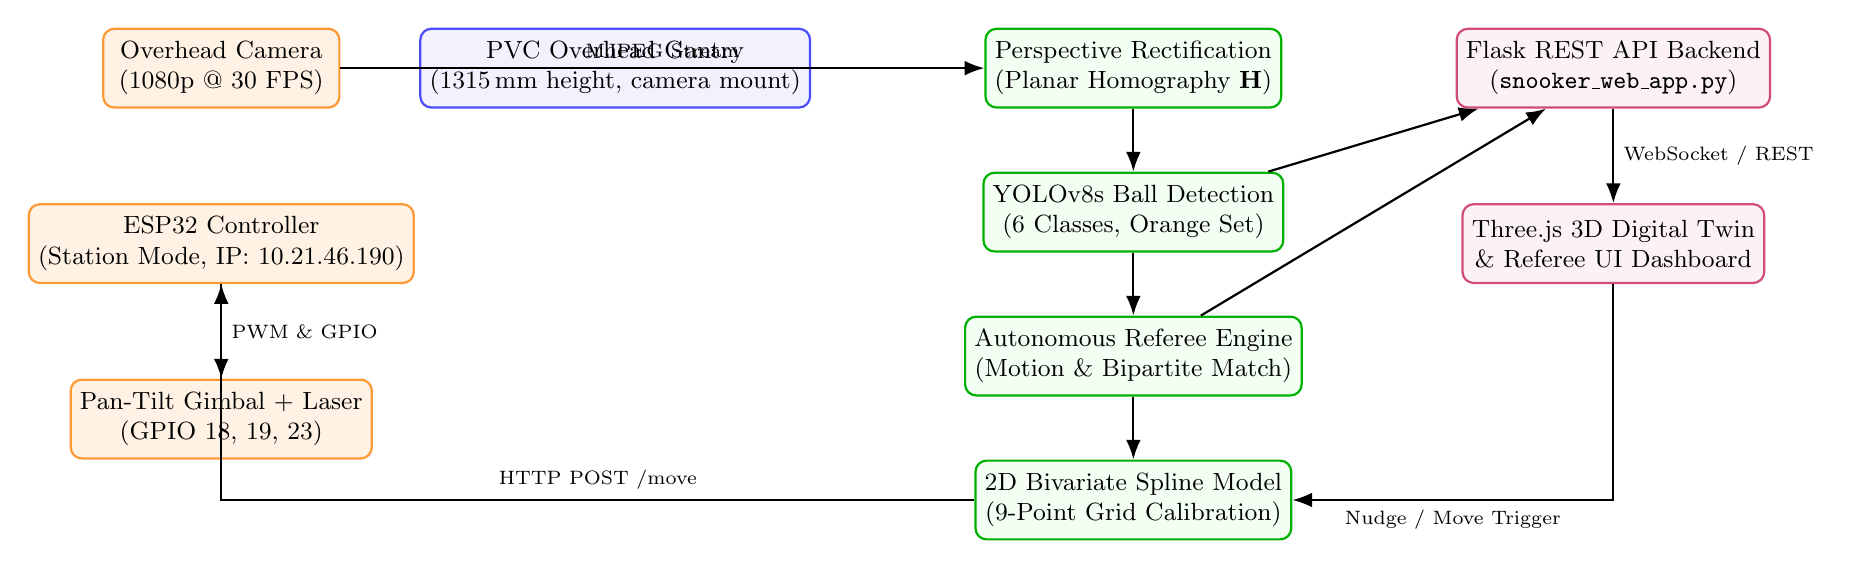
\begin{tikzpicture}[
    node distance=1.2cm and 1.0cm,
    block/.style={rectangle, draw=blue!70, fill=blue!5, thick, rounded corners, minimum height=1.0cm, minimum width=3.0cm, align=center, font=\small},
    hwblock/.style={rectangle, draw=orange!80, fill=orange!10, thick, rounded corners, minimum height=1.0cm, minimum width=3.0cm, align=center, font=\small},
    procblock/.style={rectangle, draw=green!70!black, fill=green!5, thick, rounded corners, minimum height=1.0cm, minimum width=3.2cm, align=center, font=\small},
    uiblock/.style={rectangle, draw=purple!70, fill=purple!5, thick, rounded corners, minimum height=1.0cm, minimum width=3.0cm, align=center, font=\small},
    line/.style={draw, -{Latex[length=2.5mm]}, thick}
]

% Nodes
\node[hwblock] (camera) {Overhead Camera\\(1080p @ 30 FPS)};
\node[block, right=of camera] (gantry) {PVC Overhead Gantry\\($1315\,\text{mm}$ height, camera mount)};
\node[hwblock, below=of camera] (esp32) {ESP32 Controller\\(Station Mode, IP: 10.21.46.190)};
\node[hwblock, below=of esp32] (actuator) {Pan-Tilt Gimbal + Laser\\(GPIO 18, 19, 23)};

\node[procblock, right=2.2cm of gantry] (homography) {Perspective Rectification\\(Planar Homography $\mathbf{H}$)};
\node[procblock, below=0.8cm of homography] (yolo) {YOLOv8s Ball Detection\\(6 Classes, Orange Set)};
\node[procblock, below=0.8cm of yolo] (referee) {Autonomous Referee Engine\\(Motion \& Bipartite Match)};
\node[procblock, below=0.8cm of referee] (spline) {2D Bivariate Spline Model\\(9-Point Grid Calibration)};

\node[uiblock, right=2.2cm of homography] (flask) {Flask REST API Backend\\(\texttt{snooker\_web\_app.py})};
\node[uiblock, below=1.2cm of flask] (ui) {Three.js 3D Digital Twin\\\& Referee UI Dashboard};

% Connections
\path[line] (camera) -- node[above, font=\scriptsize] {MJPEG Stream} (homography);
\path[line] (homography) -- (yolo);
\path[line] (yolo) -- (referee);
\path[line] (referee) -- (spline);
\path[line] (spline) -| node[above, near start, font=\scriptsize] {HTTP POST /move} (esp32);
\path[line] (esp32) -- node[right, font=\scriptsize] {PWM \& GPIO} (actuator);
\path[line] (yolo) -- (flask);
\path[line] (referee) -- (flask);
\path[line] (flask) -- node[right, font=\scriptsize] {WebSocket / REST} (ui);
\path[line] (ui) |- node[below, near end, font=\scriptsize] {Nudge / Move Trigger} (spline);

\end{tikzpicture}
}
\caption{System Architecture and Functional Dataflow Diagram}
\label{fig:system_architecture}
\end{figure}

Communication between the host vision computer and the embedded ESP32 microcontroller is conducted over a local 802.11 b/g/n Wi-Fi wireless network using static IP `10.21.46.190`. Listing \ref{lst:rest_api} illustrates the JSON actuation payload format.

\begin{lstlisting}[caption={ESP32 RESTful Actuation Command Payload}, label={lst:rest_api}]
POST /move HTTP/1.1
Host: 10.21.46.190
Content-Type: application/json

{
  "pan": 35.0,
  "tilt": 102.0,
  "laser": true
}
\end{lstlisting}

\section{Algorithms Used}

\subsection{Algorithm 1: Planar Projective Homography via SVD}
Accurate spatial restoration requires establishing a rigorous mathematical mapping between two-dimensional pixel coordinates $(u, v)$ on the camera image plane and real-world metric coordinates $(X_w, Y_w)$ on the snooker table \cite{ref19}. Let $\mathbf{x} = [u, v, 1]^T$ denote the homogeneous image coordinate vector and $\mathbf{X}_w = [X_w, Y_w, 1]^T$ represent the corresponding metric coordinate on the planar table surface ($Z_w = 0$). Under pinhole camera geometry, the projective mapping is governed by an invertible $3 \times 3$ homography matrix $\mathbf{H} \in \mathbb{R}^{3 \times 3}$:
\begin{equation}
    s \, \mathbf{x} = \mathbf{H} \, \mathbf{X}_w, \qquad
    \mathbf{H} = \begin{bmatrix}
        h_{11} & h_{12} & h_{13} \\
        h_{21} & h_{22} & h_{23} \\
        h_{31} & h_{32} & h_{33}
    \end{bmatrix}
    \label{eq:homography_forward}
\end{equation}
To map detected pixel positions $(u, v)$ into physical table coordinates $(X_w, Y_w)$ in millimeters, the inverse homography transformation is applied:
\begin{equation}
    \mathbf{X}_w = \mathbf{H}^{-1} \, \mathbf{x}, \qquad
    X_w = \frac{h'_{11} u + h'_{12} v + h'_{13}}{h'_{31} u + h'_{32} v + h'_{33}}, \quad
    Y_w = \frac{h'_{21} u + h'_{22} v + h'_{23}}{h'_{31} u + h'_{32} v + h'_{33}}
    \label{eq:metric_xy}
\end{equation}
where $h'_{ij}$ denotes the elements of $\mathbf{H}^{-1}$. Using four outer corner pocket correspondences $\{ (u_i, v_i) \leftrightarrow (X_{w,i}, Y_{w,i}) \}_{i=1}^4$ with $W_{\text{table}} = 1168.4\,\text{mm}$ and $L_{\text{table}} = 2341.88\,\text{mm}$, Direct Linear Transformation (DLT) constructs a homogeneous system $\mathbf{A}\mathbf{h} = \mathbf{0}$ ($\mathbf{A} \in \mathbb{R}^{8 \times 9}$), solved via Singular Value Decomposition $\mathbf{A} = \mathbf{U}\mathbf{\Sigma}\mathbf{V}^T$, where $\mathbf{h}^*$ is the right singular vector corresponding to the smallest singular value. Prior to homography mapping, Brown-Conrady radial and tangential distortion parameters are rectified \cite{ref35}.

\subsection{Algorithm 2: Spherical Elevation Parallax Compensation}
Standard homography assumes all tracked features reside on the flat table bed ($Z_w = 0$). However, snooker balls are three-dimensional spheres of diameter $D = 52.5\,\text{mm}$, so the vision detector localizes the apparent visual centroid at elevation $Z_{\text{ball}} = R = 26.25\,\text{mm}$ above the cloth. Figure \ref{fig:elevation_parallax} depicts the geometric ray propagation from the overhead optical center $(X_c, Y_c, H_{\text{cam}})$ through the elevated ball center $(X_{\text{true}}, Y_{\text{true}}, R)$ to its projected intersection $(X_{\text{obs}}, Y_{\text{obs}}, 0)$.

\begin{figure}[H]
\centering
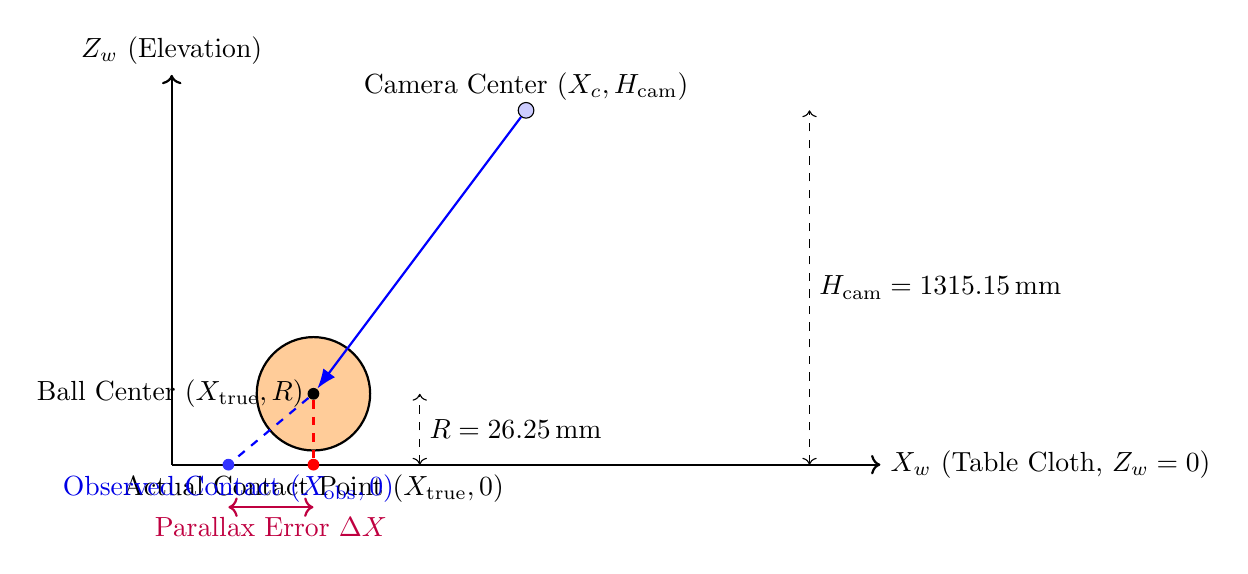
\begin{tikzpicture}[scale=0.90]
    \draw[thick, ->] (0,0) -- (10,0) node[right] {$X_w$ (Table Cloth, $Z_w=0$)};
    \draw[thick, ->] (0,0) -- (0,5.5) node[above] {$Z_w$ (Elevation)};
    \node[draw, fill=blue!20, circle, inner sep=2pt] (cam) at (5, 5) {};
    \node[above] at (cam) {Camera Center $(X_c, H_{\text{cam}})$};
    \draw[fill=orange!40, thick] (2, 1.0) circle (0.8);
    \node[fill=black, circle, inner sep=1.5pt] (ball_center) at (2, 1.0) {};
    \node[left] at (ball_center) {Ball Center $(X_{\text{true}}, R)$};
    \node[fill=red, circle, inner sep=1.5pt] (cloth_patch) at (2, 0) {};
    \node[below] at (cloth_patch) {Actual Contact Point $(X_{\text{true}}, 0)$};
    \draw[dashed, red, thick] (ball_center) -- (cloth_patch);
    \draw[thick, blue, -{Latex[length=2.5mm]}] (cam) -- (ball_center);
    \draw[dashed, blue, thick] (ball_center) -- (0.8, 0) node[fill=blue!80, circle, inner sep=1.5pt] (obs) {};
    \node[below, blue!90!black] at (obs) {Observed Contact $(X_{\text{obs}}, 0)$};
    \draw[<->, thick, purple] (0.8, -0.6) -- (2.0, -0.6);
    \node[below, purple] at (1.4, -0.6) {Parallax Error $\Delta X$};
    \draw[<->, dashed] (9, 0) -- (9, 5) node[midway, right] {$H_{\text{cam}} = 1315.15\,\text{mm}$};
    \draw[<->, dashed] (3.5, 0) -- (3.5, 1.0) node[midway, right] {$R = 26.25\,\text{mm}$};
\end{tikzpicture}
\caption{Geometric Derivation of Spherical Elevation Parallax Shift}
\label{fig:elevation_parallax}
\end{figure}

Applying similar triangles yields the closed-form true cloth contact coordinates:
\begin{align}
    X_{\text{true}} &= X_c + (X_{\text{obs}} - X_c) \left( 1 - \frac{R}{H_{\text{cam}}} \right) \label{eq:parallax_x} \\
    Y_{\text{true}} &= Y_c + (Y_{\text{obs}} - Y_c) \left( 1 - \frac{R}{H_{\text{cam}}} \right) \label{eq:parallax_y}
\end{align}
With $H_{\text{cam}} = 1315.15\,\text{mm}$ and $R = 26.25\,\text{mm}$, the scaling factor is $\gamma = 1 - 26.25/1315.15 \approx 0.98004$, neutralizing up to $\Delta X \approx 12.0\,\text{mm}$ of radial corner parallax.

\subsection{Algorithm 3: Dual-Axis Inverse Kinematics and 2D Bivariate Cubic Spline Calibration}
Targeting a point $\mathbf{P} = (X_w, Y_w, 0)$ from the top-right gimbal origin $(X_0, Y_0, Z_0) = (0, 0, H_{\text{gimbal}})$ yields ideal trigonometric inverse kinematics:
\begin{align}
    \theta_{\text{pan}}^{\text{ideal}} &= \arctan2(Y_w - Y_0, \, X_w - X_0) \label{eq:pan_ideal} \\
    \phi_{\text{tilt}}^{\text{ideal}} &= \arctan2\left( \sqrt{(X_w - X_0)^2 + (Y_w - Y_0)^2}, \, Z_0 \right) \label{eq:tilt_ideal}
\end{align}
Because physical servos exhibit potentiometer non-linearities, horn mounting offsets, gear backlash, and gravity droop, theoretical equations produce errors exceeding $\pm 22\,\text{mm}$. To eliminate these non-linearities, the table is discretized into a 9-point spatial calibration grid ($P_1$ through $P_9$: pockets, cushion midpoints, and center node). Ground-truth servo angles $\{ (\theta_k, \phi_k) \}_{k=1}^9$ are recorded via live nudge controls, and two independent 2D bivariate cubic spline functions are fitted:
\begin{align}
    \theta_{\text{pan}}(X_w, Y_w) &= \sum_{i=1}^m \sum_{j=1}^n c_{ij}^{\text{pan}} \, B_i(X_w) \, B_j(Y_w) \label{eq:spline_pan} \\
    \phi_{\text{tilt}}(X_w, Y_w) &= \sum_{i=1}^m \sum_{j=1}^n c_{ij}^{\text{tilt}} \, B_i(X_w) \, B_j(Y_w) \label{eq:spline_tilt}
\end{align}
where $B_i(X)$ and $B_j(Y)$ are cubic B-spline basis functions obtained by minimizing the penalized sum of squares, achieving $\pm 2.18\,\text{mm}$ mean laser repeatability.

\subsection{Algorithm 4: Hungarian Bipartite Matching for Ball State Differencing}
Because the fifteen orange object balls are visually identical, simple class-based tracking fails after multi-ball collisions. Let $\mathcal{S}_{\text{pre}} = \{ \mathbf{p}_i^{\text{pre}} \}_{i=1}^{N}$ and $\mathcal{S}_{\text{post}} = \{ \mathbf{p}_j^{\text{post}} \}_{j=1}^{M}$ denote pre-shot and post-shot coordinates. A cost matrix $\mathbf{C} \in \mathbb{R}^{N \times M}$ is built using Euclidean distances $C_{ij} = \| \mathbf{p}_i^{\text{pre}} - \mathbf{p}_j^{\text{post}} \|_2$ (with $C_{ij} = \infty$ across mismatched ball classes). The optimal one-to-one assignment is solved via the Hungarian Algorithm \cite{ref40}:
\begin{equation}
    \min_{\mathbf{X}} \sum_{i=1}^N \sum_{j=1}^M C_{ij} X_{ij} \quad \text{subject to} \quad \sum_{j=1}^M X_{ij} \le 1, \; \sum_{i=1}^N X_{ij} \le 1, \; X_{ij} \in \{0, 1\}
\end{equation}
Matched pairs with $C_{ij} \le \tau_{\text{stationary}} = 10.0\,\text{mm}$ are classified as \textbf{Stationary}; pairs with $C_{ij} > 10.0\,\text{mm}$ are flagged as \textbf{Displaced} ($\mathbf{d}_i = \mathbf{p}_j^{\text{post}} - \mathbf{p}_i^{\text{pre}}$); unmatched pre-shot balls are marked \textbf{Potted}.

\subsection{Algorithm 5: Autonomous Referee Finite State Machine (FSM)}
The autonomous referee operates as a five-state FSM (Figure \ref{fig:fsm_diagram}): \textbf{State 0 (Idle/Armed)} locks the pre-shot baseline; \textbf{State 1 (Shot Motion)} triggers when inter-frame motion exceeds $\Delta I > 5.0\%$; \textbf{State 2 (Settlement Timer)} enforces a $2.5\,\text{s}$ stability countdown once motion falls below $0.8\%$; \textbf{State 3 (State Diffing)} runs YOLOv8s and Hungarian matching; and \textbf{State 4 (Laser Restoration)} sequentially steers the laser diode to each displaced ball's $\mathbf{p}_i^{\text{pre}}$ coordinate upon a foul call.

\begin{figure}[H]
\centering
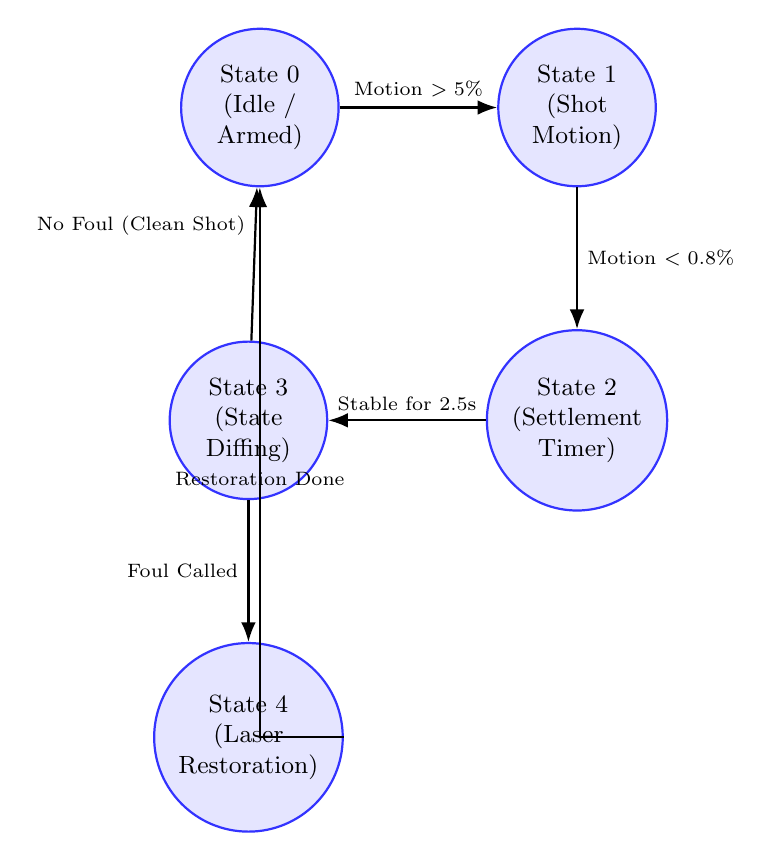
\begin{tikzpicture}[
    node distance=1.8cm,
    state/.style={draw=blue!80, fill=blue!10, circle, thick, minimum size=2.0cm, align=center, font=\small},
    line/.style={draw, -{Latex[length=2.5mm]}, thick}
]
\node[state] (s0) {State 0\\(Idle /\\Armed)};
\node[state, right=2.0cm of s0] (s1) {State 1\\(Shot\\Motion)};
\node[state, below=1.8cm of s1] (s2) {State 2\\(Settlement\\Timer)};
\node[state, left=2.0cm of s2] (s3) {State 3\\(State\\Diffing)};
\node[state, below=1.8cm of s3] (s4) {State 4\\(Laser\\Restoration)};

\path[line] (s0) -- node[above, font=\scriptsize] {Motion $>5\%$} (s1);
\path[line] (s1) -- node[right, font=\scriptsize] {Motion $<0.8\%$} (s2);
\path[line] (s2) -- node[above, font=\scriptsize] {Stable for 2.5s} (s3);
\path[line] (s3) -- node[left, font=\scriptsize] {Foul Called} (s4);
\path[line] (s3) -- node[left, near end, font=\scriptsize] {No Foul (Clean Shot)} (s0);
\path[line] (s4) -| node[below, near end, font=\scriptsize] {Restoration Done} (s0);
\end{tikzpicture}
\caption{Finite State Machine (FSM) Diagram of Autonomous Referee Workflow}
\label{fig:fsm_diagram}
\end{figure}

\section{Tools and Technologies}
Table \ref{tab:hardware_bom} details the complete Hardware Bill of Materials (BOM) and approximate prototype expenditure in Indian Rupees (INR).

\begin{table}[H]
\centering
\caption{Hardware Bill of Materials (BOM) and Cost Breakdown}
\label{tab:hardware_bom}
\resizebox{\textwidth}{!}{
\begin{tabular}{|c|l|l|c|r|}
\hline
\textbf{Sl. No.} & \textbf{Component Name} & \textbf{Technical Specifications / Ratings} & \textbf{Qty} & \textbf{Cost (INR)} \\
\hline
1 & Custom Snooker Table & $1168.4\,\text{mm} \times 2341.88\,\text{mm}$, green tournament felt, 6 pockets & 1 & 12,500.00 \\
2 & Overhead PVC Gantry & Class-B $1.0''$ Schedule 40 PVC pipes, 90$^\circ$ elbows, T-joints, height $1315.15\,\text{mm}$ & 1 Set & 1,850.00 \\
3 & Overhead Camera Unit & Full HD 1080p CMOS sensor, wide-angle distortion-free lens, USB/Wi-Fi RTSP & 1 & 2,200.00 \\
4 & ESP32 Dev Kit & 30-pin ESP-WROOM-32, Dual-Core 240MHz, 520KB SRAM, 802.11 b/g/n Wi-Fi & 1 & 550.00 \\
5 & Pan-Tilt Metal Brackets & Heavy-duty black anodized aluminum 2-DOF pan-tilt servo bracket kit & 1 Set & 450.00 \\
6 & Servos (Pan \& Tilt) & TowerPro MG996R high-torque metal gear servos ($11\,\text{kg}\cdot\text{cm}$ @ 6V, $180^\circ$) & 2 & 780.00 \\
7 & Red Laser Diode & $650\,\text{nm}$, 5mW, operating voltage 3.0V--5.0V DC, focused dot brass casing & 1 & 120.00 \\
8 & Power MOSFET Driver & IRFZ44N N-Channel Power MOSFET ($V_{DSS}=55\,\text{V}$, $I_D=49\,\text{A}$, $R_{DS(on)}=17.5\,\text{m}\Omega$) & 1 & 45.00 \\
9 & Gate Pull-Down Resistor & $10\,\text{k}\Omega$ 1/4W $\pm 1\%$ Metal Film Resistor (MOSFET gate stabilization) & 1 & 5.00 \\
10 & DC-DC Buck Converter & LM2596 / XL4015 step-down regulator (12V input, trimmer tuned to steady 6.0V output) & 1 & 180.00 \\
11 & Main Power Supply & 12V 5A (60 Watts) regulated switch-mode DC adapter, 2.1mm $\times$ 5.5mm jack & 1 & 650.00 \\
12 & Prototyping Breadboards & 830-tie point / 400-tie point solderless breadboards with dual power rails & 2 & 260.00 \\
13 & Screw Terminal Blocks & 2-pin / multi-terminal PCB screw breakout blocks for high-current 12V/6V rails & 3 & 60.00 \\
14 & Regulation Snooker Balls & $52.5\,\text{mm}$ phenolic resin balls (Active: Orange set, White, Yellow, Green, Blue, Pink) & 1 Set & 1,650.00 \\
15 & Wooden Electronics Stand & Elevated side support stand for control electronics, laptop, and gantry base & 1 & 750.00 \\
16 & Connecting Hardware & Jumper wires, heat shrink tubing, zip ties, mounting nuts and bolts & 1 Set & 200.00 \\
\hline
\multicolumn{4}{|r|}{\textbf{Total Prototype Expenditure (INR):}} & \textbf{21,800.00} \\
\hline
\end{tabular}
}
\end{table}

The software stack comprises:
\begin{itemize}
    \item \textbf{Host Vision \& Scientific Computing:} Windows 11 / Ubuntu 22.04 LTS, Python 3.10, PyTorch 2.0.1 (CUDA), Ultralytics YOLOv8s, OpenCV 4.8.0, NumPy 1.24.3, and SciPy 1.10.1 (\texttt{RectBivariateSpline}, \texttt{linear\_sum\_assignment}).
    \item \textbf{Embedded Firmware:} Arduino IDE / PlatformIO with Espressif ESP32 core (v2.0.11), \texttt{WebServer}, and \texttt{ESP32Servo} PWM hardware timer libraries.
    \item \textbf{Backend \& Frontend Web Stack:} Flask 3.0 multi-threaded REST server, HTML5/CSS3/ES6+ JavaScript, and Three.js (r128) WebGL engine.
\end{itemize}

\chapter{IMPLEMENTATION AND TESTING}

\section{System Implementation}
The cyber-physical snooker ball identification and laser positioning platform is implemented as six modular subsystems spanning mechanical rig fabrication, embedded power electronics, deep learning computer vision, RESTful middleware, 3D WebGL visualization, and autonomous refereeing.

\subsection{Module 1: Physical Table and Overhead PVC Gantry Construction}
To create a dependable, rigid experimental platform that conforms to institutional laboratory space constraints while faithfully replicating professional snooker dynamics, a custom snooker table and overhead gantry were constructed.

\subsection{Table Specifications and Playing Surface}
The physical snooker table features an active playing surface measuring:
\begin{itemize}
    \item \textbf{Internal Playing Width ($W_{\text{table}}$):} $1168.4\,\text{mm}$ ($46.0\,\text{inches}$)
    \item \textbf{Internal Playing Length ($L_{\text{table}}$):} $2341.88\,\text{mm}$ ($92.2\,\text{inches}$)
    \item \textbf{Aspect Ratio:} Exactly $1:2.004$, mirroring regulation cue sports proportions.
    \item \textbf{Cushion Railing and Pockets:} Six regulation pockets (four corner pockets and two center pockets) lined with drop nets and leather impact bevels.
    \item \textbf{Cloth and Baize:} High-density tournament green wool-nylon blend felt stretched over a leveled bed, providing uniform rolling resistance.
\end{itemize}

\subsection{Structural PVC Overhead Gantry}
To eliminate floor obstructions around the playing perimeter while ensuring complete visual coverage of the $1168.4 \times 2341.88\,\text{mm}$ surface, an overhead structural gantry was engineered using high-grade $1.0\text{-inch}$ Schedule-40 Polyvinyl Chloride (PVC) piping. 

As shown in Figures \ref{fig:rig_setup} and \ref{fig:rig_overhead}, the gantry structure features:
\begin{itemize}
    \item \textbf{Vertical Clear Height:} $1315.15\,\text{mm}$ ($51.78\,\text{inches}$) clearance from the table bed to the overhead transverse crossbars.
    \item \textbf{Four Corner Uprights:} Dual-tube vertical columns reinforced with transverse T-connectors to prevent mechanical sway, torsion, and vibration.
    \item \textbf{Overhead Transverse Beam:} Houses the central downward-facing Full HD camera mount, aligned with the geometric center of the table.
\end{itemize}

\begin{figure}[H]
    \centering
    \begin{subfigure}[b]{0.48\textwidth}
        \centering
        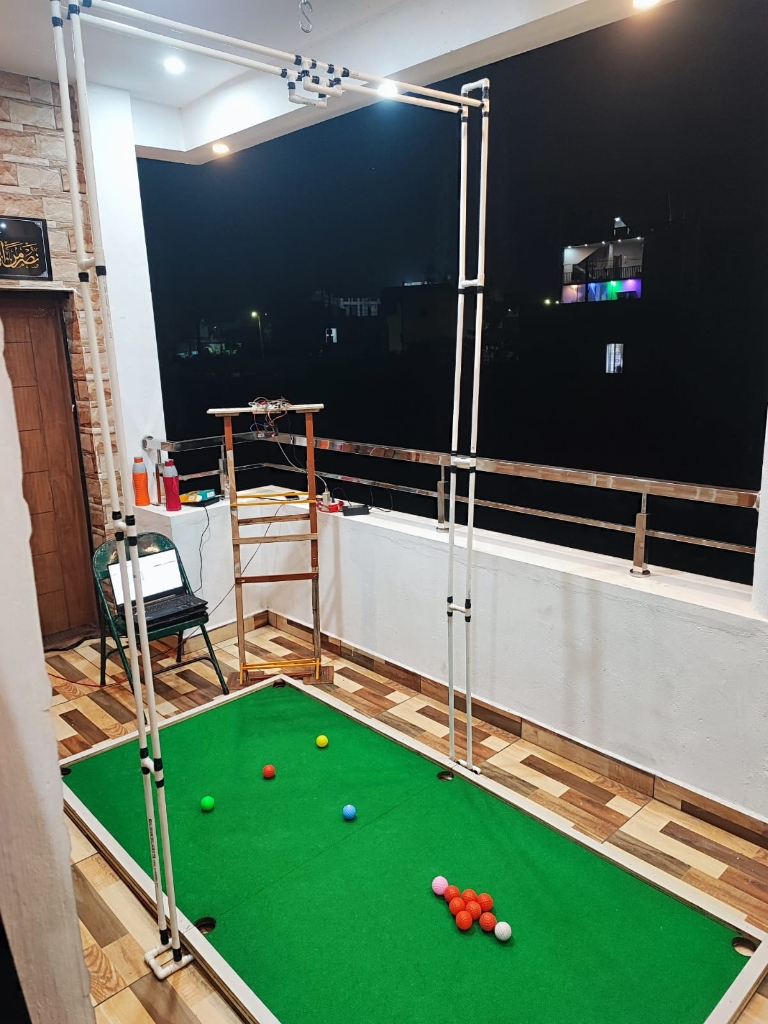
\includegraphics[width=\textwidth]{rig_setup_perspective.jpg}
        \caption{Perspective view of PVC gantry, lighting, and table}
        \label{fig:rig_setup}
    \end{subfigure}
    \hfill
    \begin{subfigure}[b]{0.48\textwidth}
        \centering
        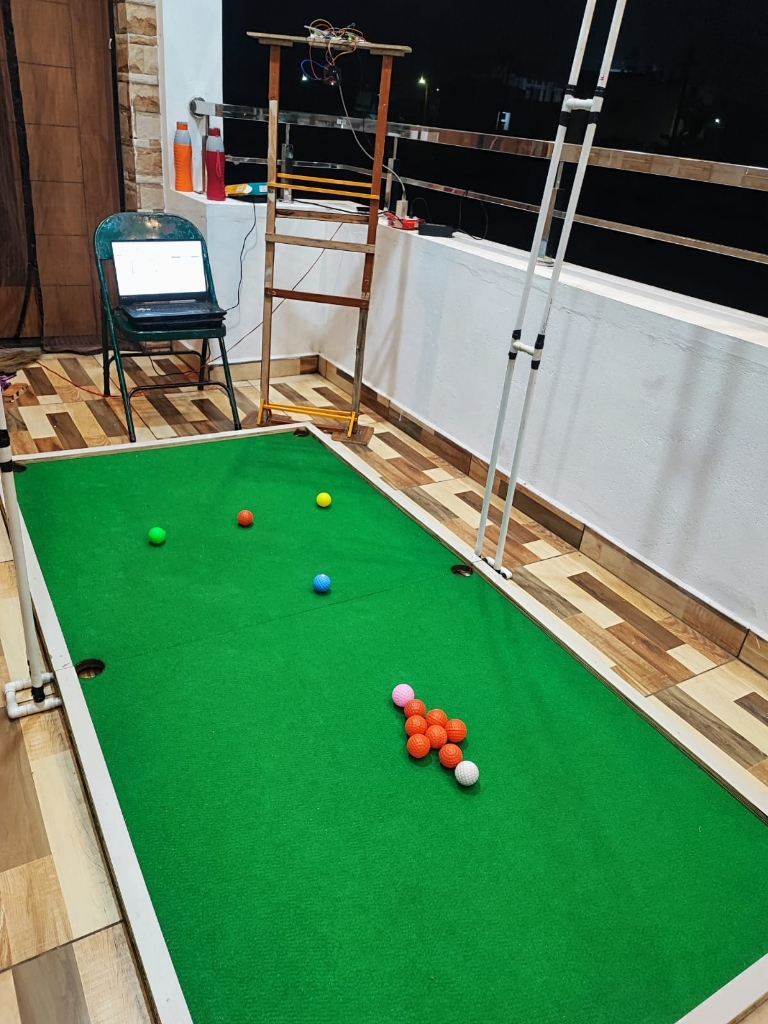
\includegraphics[width=\textwidth]{rig_gantry_overhead.jpg}
        \caption{Overhead view showing top-down camera frame}
        \label{fig:rig_overhead}
    \end{subfigure}
    \caption{Physical Hardware Rig: Custom Table, Overhead PVC Gantry, and Illumination}
    \label{fig:physical_hardware_rig}
\end{figure}

\subsection{Active Ball Set and Color Strategy}
In our prototype setup, a specialized ball configuration was adopted:
\begin{itemize}
    \item \textbf{Diameter:} Regulation $52.5\,\text{mm}$ phenolic resin spheres.
    \item \textbf{Object Balls (Orange Set):} High-visibility dimpled/smooth orange balls were deployed in place of traditional dark red balls. As illustrated in Figures \ref{fig:table_topdown} and \ref{fig:table_overview}, orange spheres provide superior chrominance contrast against green tournament cloth, maximizing the signal-to-noise ratio in the YOLOv8 convolutional feature space.
    \item \textbf{Color Balls:} Standard tournament colors: White (Cue Ball), Yellow (2 pts), Green (3 pts), Blue (5 pts), and Pink (6 pts).
\end{itemize}

\begin{figure}[H]
    \centering
    \begin{subfigure}[b]{0.48\textwidth}
        \centering
        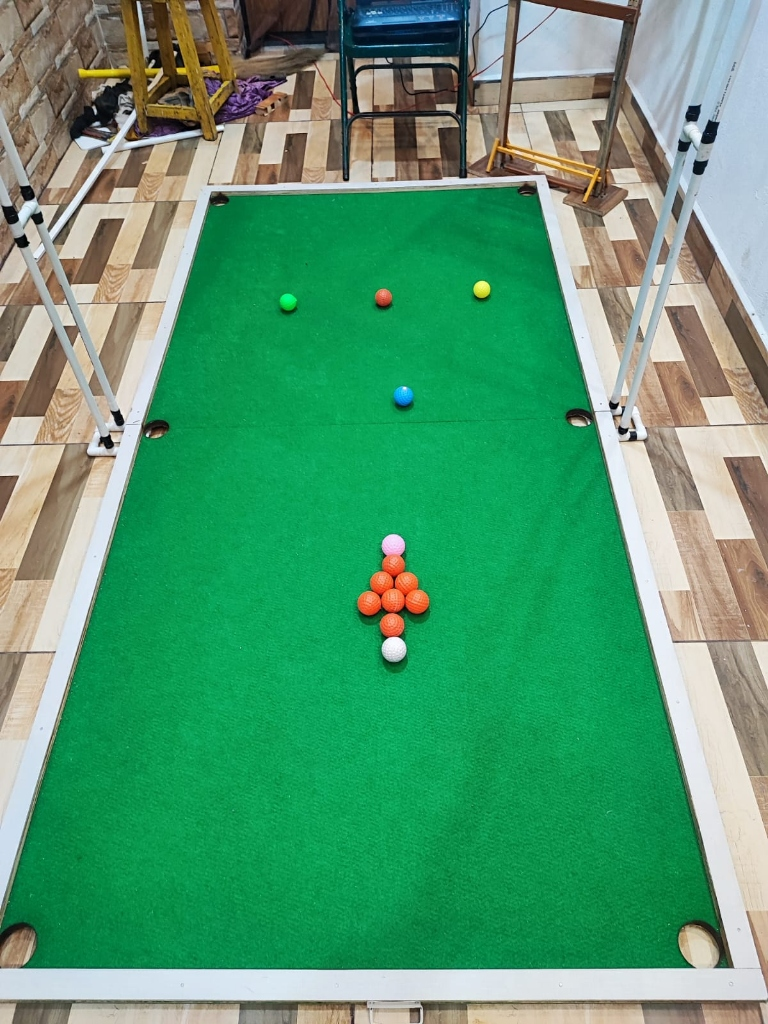
\includegraphics[width=\textwidth]{table_topdown_balls.jpg}
        \caption{Top-down longitudinal view of table cloth and rack}
        \label{fig:table_topdown}
    \end{subfigure}
    \hfill
    \begin{subfigure}[b]{0.48\textwidth}
        \centering
        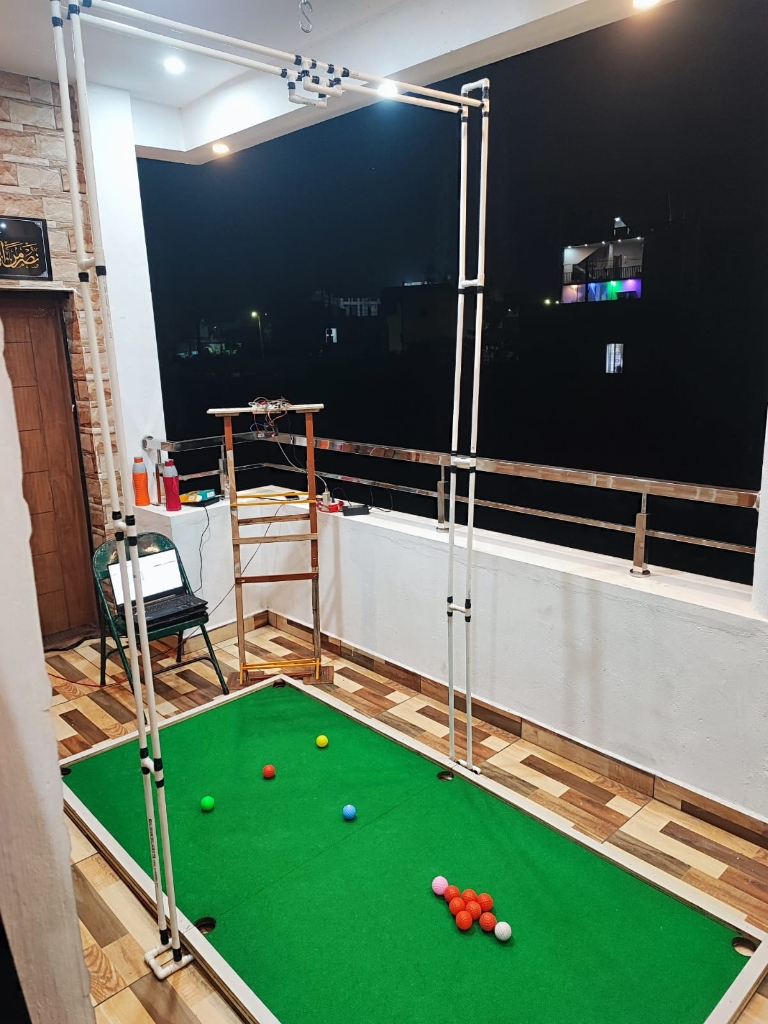
\includegraphics[width=\textwidth]{physical_table_overview.jpg}
        \caption{Overview of table, control laptop, and side rig}
        \label{fig:table_overview}
    \end{subfigure}
    \caption{Physical Snooker Playing Surface and Active Ball Set Deployment}
    \label{fig:physical_balls_table}
\end{figure}

\section{Embedded Hardware and Mechatronics Implementation}
The physical actuation and optical projection subsystem combines robust mechatronics, dedicated power regulation, high-current switching, and real-time microcontroller firmware. Figure \ref{fig:hardware_mechatronics_photos} shows the real physical assembly of both the dual-servo pan-tilt gimbal and the completed breadboard circuit.

\begin{figure}[H]
    \centering
    \begin{subfigure}[b]{0.48\textwidth}
        \centering
        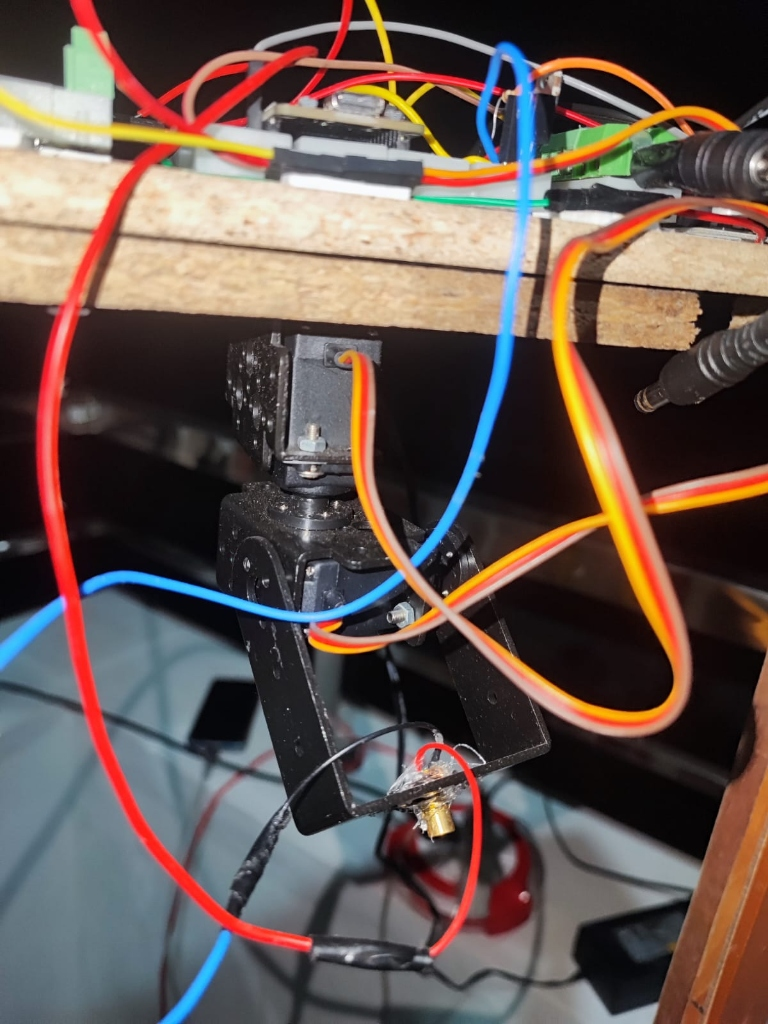
\includegraphics[width=\textwidth]{hardware_pantilt_assembly.jpg}
        \caption{Dual MG996R metal-gear servos in aluminum pan-tilt bracket with laser diode}
        \label{fig:hw_pantilt}
    \end{subfigure}
    \hfill
    \begin{subfigure}[b]{0.48\textwidth}
        \centering
        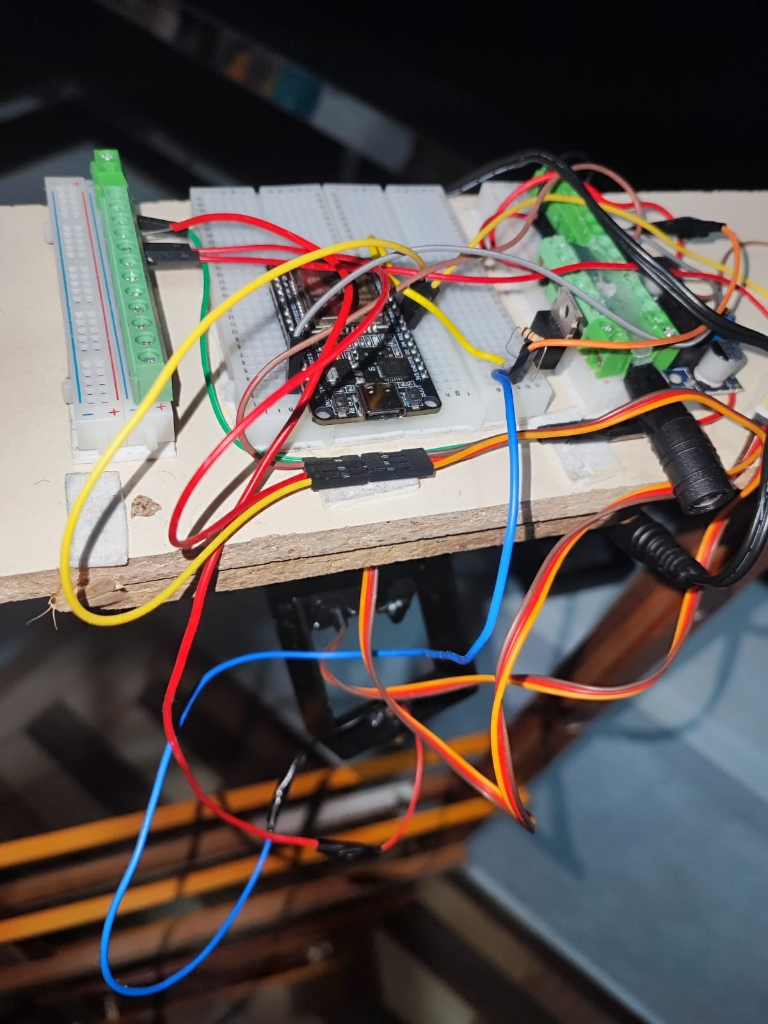
\includegraphics[width=\textwidth]{hardware_circuit_breadboard.jpg}
        \caption{Breadboard electronics: ESP32 Dev Kit, DC-DC buck converter, IRFZ44N MOSFET, and terminal blocks}
        \label{fig:hw_circuit}
    \end{subfigure}
    \caption{Physical Mechatronics and Embedded Circuit Assembly}
    \label{fig:hardware_mechatronics_photos}
\end{figure}

\subsection{Pan-Tilt Gimbal and MG996R Metal Gear Servos}
As shown in Figure \ref{fig:hw_pantilt}, the optical pointer is constructed using heavy-duty black anodized aluminum pan-tilt brackets suspended beneath the wooden side platform:
\begin{itemize}
    \item \textbf{High-Torque Metal Gear Servos:} Two TowerPro MG996R metal-gear servos provide the azimuth (Pan) and elevation (Tilt) motions. Compared to standard plastic-gear micro-servos, the MG996R features full steel and brass gearing delivering an exceptional stall torque of $11.0\,\text{kg}\cdot\text{cm}$ at $6.0\,\text{V}$. This completely eliminates the gear stripping, backlash play, and cantilevered sagging observed in lightweight servos over long table distances.
    \item \textbf{Laser Diode Mount:} A $650\,\text{nm}$ red focused dot laser diode module ($5\,\text{mW}$) is securely seated in the central bracket holder, locked with thermal adhesive to maintain bore-sight alignment across repeated rapid servo rotations.
\end{itemize}

\subsection{Circuit Architecture, Power Regulation, and MOSFET Switching}
The electronic control system shown in Figure \ref{fig:hw_circuit} is built across two solderless prototyping breadboards equipped with industrial screw terminal blocks for high-current routing:
\begin{enumerate}
    \item \textbf{12V 5A Master Power Supply:} A 12V 5A (60 Watts) switch-mode DC power adapter provides primary power via a standard $2.1\,\text{mm} \times 5.5\,\text{mm}$ barrel jack into the primary screw terminal block.
    \item \textbf{DC-DC Buck Converter (6.0V Bus):} Because the two MG996R servos draw up to $1.2\,\text{A}$ stall current each during acceleration, an onboard high-efficiency DC-to-DC step-down buck converter (LM2596 / XL4015) steps down the $12\,\text{V}$ input to a steady, regulated $6.0\,\text{V}$ DC bus. This isolated high-current bus directly feeds the servos, completely eliminating the voltage drops and brownout resets that occur when servos share a linear 5V logic regulator.
    \item \textbf{ESP32 Dev Kit Microcontroller:} The 30-pin ESP-WROOM-32 development board is powered through its VIN/USB port, sharing a common ground plane with the $6.0\,\text{V}$ and $12\,\text{V}$ supplies.
    \item \textbf{IRFZ44N Power MOSFET Laser Driver:} To isolate the ESP32 GPIO logic and ensure clean, high-speed switching of the laser diode without loading the microcontroller, an IRFZ44N N-Channel Power MOSFET ($V_{DSS} = 55\,\text{V}$, $I_D = 49\,\text{A}$, $R_{DS(on)} = 17.5\,\text{m}\Omega$) is deployed in a low-side switching configuration:
    \begin{itemize}
        \item The MOSFET Gate is driven by ESP32 GPIO 23.
        \item A $10\,\text{k}\Omega$ metal film pull-down resistor is wired between Gate and GND, ensuring that the gate is held securely at logic LOW ($0\,\text{V}$) during ESP32 bootup, flash programming, or Wi-Fi initialization.
        \item The Drain pin sinks the laser diode cathode, while the laser anode connects to the positive power rail through a current-limiting resistor.
        \item When GPIO 23 outputs HIGH ($3.3\,\text{V}$), the MOSFET channel fully conducts with negligible internal resistance, instantaneously illuminating the laser beam with maximum optical coherence.
    \end{itemize}
\end{enumerate}

\subsection{Embedded Firmware Architecture (ESP32 Station Mode)}
The embedded firmware executes on the ESP32 utilizing FreeRTOS tasks and the `ESP32Servo` library:
\begin{itemize}
    \item \textbf{Wi-Fi Station Mode:} The ESP32 connects directly to the dedicated local wireless network with static IP `10.21.46.190`, providing low-latency packet transmission ($\sim 34\,\text{ms}$).
    \item \textbf{Hardware Timer PWM:} Channels 0 and 1 on Timer 0 generate stable $50\,\text{Hz}$ PWM control pulses ($500\,\mu\text{s}$ to $2500\,\mu\text{s}$) on GPIO 18 (Pan) and GPIO 19 (Tilt) with 16-bit resolution.
    \item \textbf{RESTful Web Server:} Implements an asynchronous HTTP server handling \texttt{POST /move}, \texttt{GET /status}, and \texttt{GET /laser?state=0|1}.
    \item \textbf{Safety Watchdog:} Automatically shuts down the laser diode if no commands are received within $120\,\text{seconds}$, complying with optical eye-safety standards.
\end{itemize}

\section{Computer Vision Pipeline (YOLOv8s)}
Object detection is driven by Ultralytics YOLOv8s (Small), an anchor-free single-stage detector characterized by high detection precision and edge-device inference speed \cite{ref11, ref12}.

\subsection{Model Training and Dataset Annotation}
The model was fine-tuned on a custom dataset of 1,850 annotated snooker table images captured under varied lighting, ball positions, and cluster densities. Bounding boxes were manually annotated across six classes:
\begin{enumerate}
    \item \texttt{orange ball} (Object balls, 1 point)
    \item \texttt{white ball} (Cue ball)
    \item \texttt{yellow ball} (2 points)
    \item \texttt{green ball} (3 points)
    \item \texttt{blue ball} (5 points)
    \item \texttt{pink ball} (6 points)
\end{enumerate}
Training was executed on an NVIDIA GPU workstation over 100 epochs using the AdamW optimizer, cosine learning rate scheduling ($lr_0 = 0.01$), mosaic augmentation, and multi-scale resizing ($1024 \times 1024$ pixels).

\subsection{Inference and Non-Maximum Suppression (NMS)}
During live operation, raw camera frames are resized to $1024 \times 1024$ and fed to the YOLOv8s inference engine. Detections undergo Non-Maximum Suppression (NMS) with an IoU threshold of $0.45$ and a confidence threshold of $0.50$, outputting bounding boxes $(x_1, y_1, x_2, y_2)$, class label $c_k$, and prediction score $s_k$. Centroid pixel coordinates are computed as:
\begin{equation}
    u_c = \frac{x_1 + x_2}{2}, \quad v_c = \frac{y_1 + y_2}{2}
\end{equation}

\section{Backend Server Architecture (Flask)}
The backend system (\texttt{snooker\_web\_app.py}) is implemented using Python and Flask, orchestrating video stream processing, coordinate transformations, and REST communication with the ESP32.

\subsection{Video Streaming and Offline Fault Resilience}
The overhead camera feed is accessed via an RTSP/MJPEG network stream. To prevent server blocking during network drops or when the camera phone is switched off, a multi-threaded streaming proxy was implemented:
\begin{itemize}
    \item \textbf{Low Socket Timeout:} HTTP socket reads are capped at $1.2\,\text{seconds}$.
    \item \textbf{Offline Frame Cache:} If the live camera stream disconnects, the backend seamlessly serves a cached reference table image (`photo58.jpg`) annotated with an ``OFFLINE / CACHED FEED'' badge. This allows all web application tabs, 3D simulations, and calibration routines to remain fully operable without runtime crashes.
\end{itemize}

\subsection{API Routing}
Key REST endpoints exposed by the Flask backend include:
\begin{itemize}
    \item \texttt{GET /api/camera/stream}: Streams live MJPEG video frames to the web UI.
    \item \texttt{POST /api/table/corners}: Saves the four calibrated pixel corner fiducials and computes the $3 \times 3$ homography matrix $\mathbf{H}$.
    \item \texttt{POST /api/laser/move}: Computes spline-interpolated servo angles and dispatches an HTTP request to `http://10.21.46.190/move`.
    \item \texttt{POST /api/laser/nudge}: Applies micro-trim increments ($\pm 0.2^\circ$ or $\pm 1.0^\circ$) to current pan/tilt angles.
    \item \texttt{POST /api/referee/analyze\_shot}: Triggers YOLOv8 detection, compares pre/post states, and returns displaced ball vectors.
\end{itemize}

\section{Interactive 3D Digital Twin and User Interface}
The front-end user interface is implemented as a single-page responsive dashboard providing full supervisory control over the physical and virtual table states.

\subsection{Three.js 3D Virtual Table Twin}
Using Three.js WebGL, a geometrically accurate 3D model of the snooker table was developed:
\begin{itemize}
    \item Real-world metric dimensions ($1168.4 \times 2341.88\,\text{mm}$) scaled into 3D units.
    \item Six modeled regulation drop pockets with dark inner recesses.
    \item Tournament baulk line ($737\,\text{mm}$ from bottom cushion) and semi-circular 'D' zone ($292\,\text{mm}$ radius).
    \item Dynamically rendered 3D ball meshes positioned in real-time according to YOLO detections, colored accurately by class.
    \item Virtual laser ray projected from the top-right gantry mast to the selected target coordinate on the cloth, displaying live calculated pan/tilt angles.
    \item OrbitControls allowing free perspective orbiting, top-down bird's eye view, and player eye-level inspection.
\end{itemize}

\subsection{Tabbed Interface Modules}
As evidenced in Figures \ref{fig:ui_3d} to \ref{fig:ui_yolo}, the web application organizes system functionality into six intuitive tabs:
\begin{enumerate}
    \item \textbf{Tab 1 (3D Table View \& Click-to-Aim):} Displays the interactive 3D digital twin alongside a target positioning panel with quick preset buttons for pockets, center spots, and live fine-tuning nudge controls (Figures \ref{fig:ui_3d} and \ref{fig:ui_laser}).
    \item \textbf{Tab 2 (Camera \& Homography):} Features an interactive canvas where the referee clicks table corner pockets to compute and verify the homography matrix $\mathbf{H}$ (Figure \ref{fig:ui_homography}).
    \item \textbf{Tab 3 (Servo \& Laser Controls):} Exposes direct hardware sliders, IP configuration (`10.21.46.190`), ping latency diagnostics, and laser safety overrides (Figure \ref{fig:ui_servo}).
    \item \textbf{Tab 4 (Ball Detection \& YOLO):} Displays raw camera frames with overlaid YOLOv8 bounding boxes, detection confidence tags, metric $(X_w, Y_w)$ coordinates, and individual ``Aim Laser'' buttons for every ball (Figure \ref{fig:ui_yolo}).
    \item \textbf{Tab 5 (Foul Detection \& Autonomous Referee):} Displays real-time video motion percentages, automated pre/post shot state transitions, and a table of displaced balls with one-click laser restoration actions (Figure \ref{fig:ui_referee}).
    \item \textbf{Tab 6 (9-Point Calibration Wizard):} Guided interface for recording empirical servo angles across the nine reference table nodes to update the 2D bivariate cubic spline model (Figure \ref{fig:ui_calib}).
\end{enumerate}

\begin{figure}[H]
    \centering
    \begin{subfigure}[b]{0.48\textwidth}
        \centering
        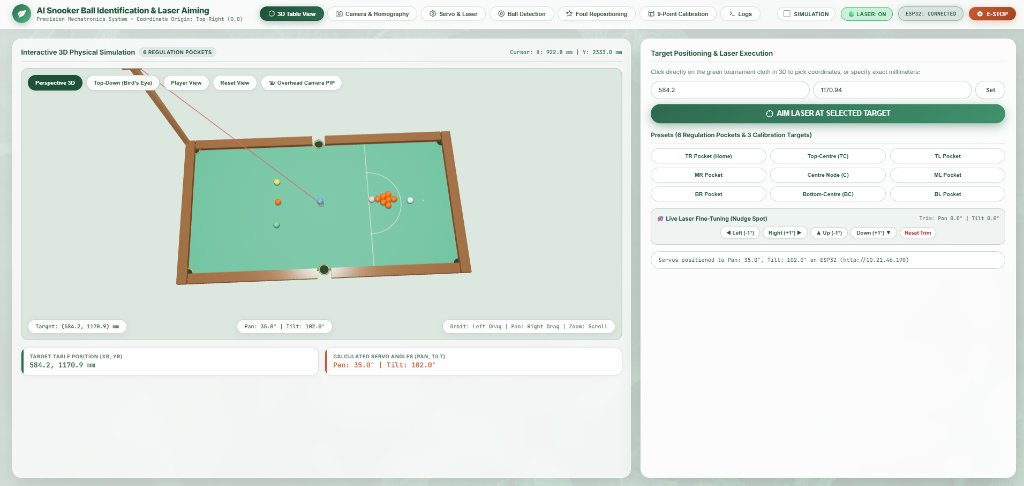
\includegraphics[width=\textwidth]{ui_3d_table.png}
        \caption{Tab 1: Interactive Three.js 3D Virtual Table Twin}
        \label{fig:ui_3d}
    \end{subfigure}
    \hfill
    \begin{subfigure}[b]{0.48\textwidth}
        \centering
        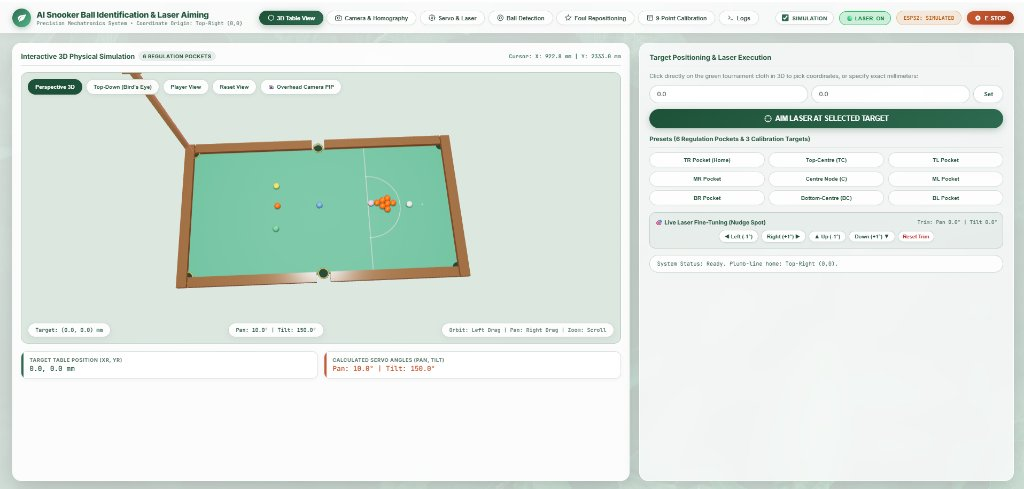
\includegraphics[width=\textwidth]{ui_laser_aiming.png}
        \caption{Tab 1: Target Positioning and Live Laser Aiming}
        \label{fig:ui_laser}
    \end{subfigure}
    \caption{Web Application Interface: 3D Simulation and Target Execution}
    \label{fig:ui_views_1}
\end{figure}

\begin{figure}[H]
    \centering
    \begin{subfigure}[b]{0.48\textwidth}
        \centering
        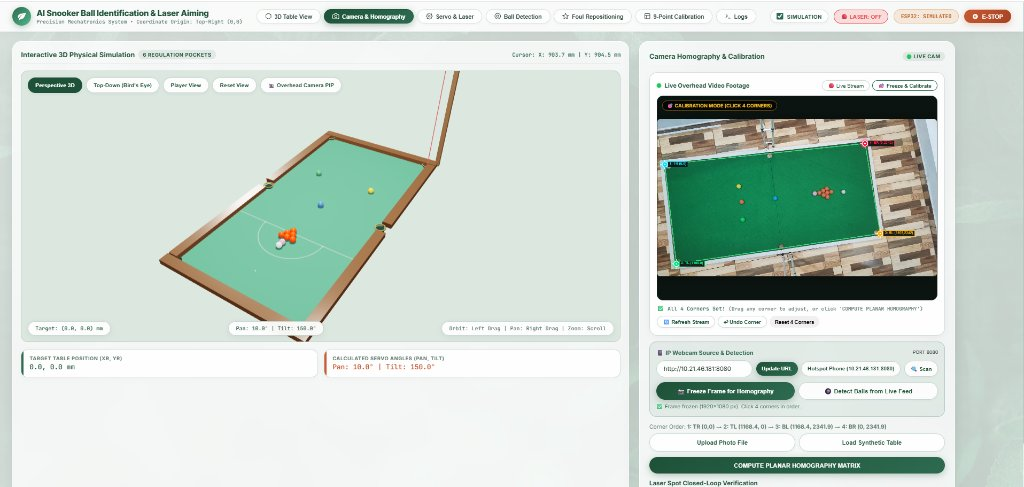
\includegraphics[width=\textwidth]{ui_camera_homography.png}
        \caption{Tab 2: Planar Homography 4-Point Corner Calibration}
        \label{fig:ui_homography}
    \end{subfigure}
    \hfill
    \begin{subfigure}[b]{0.48\textwidth}
        \centering
        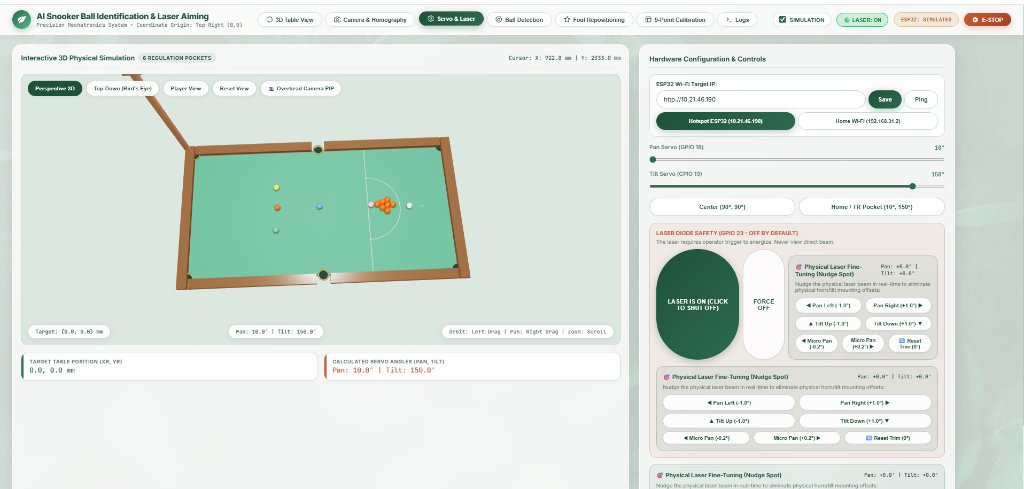
\includegraphics[width=\textwidth]{ui_servo_laser.png}
        \caption{Tab 3: Hardware Servo Sliders and Laser Controls}
        \label{fig:ui_servo}
    \end{subfigure}
    \caption{Web Application Interface: Calibration and Hardware Controls}
    \label{fig:ui_views_2}
\end{figure}

\begin{figure}[H]
    \centering
    \begin{subfigure}[b]{0.48\textwidth}
        \centering
        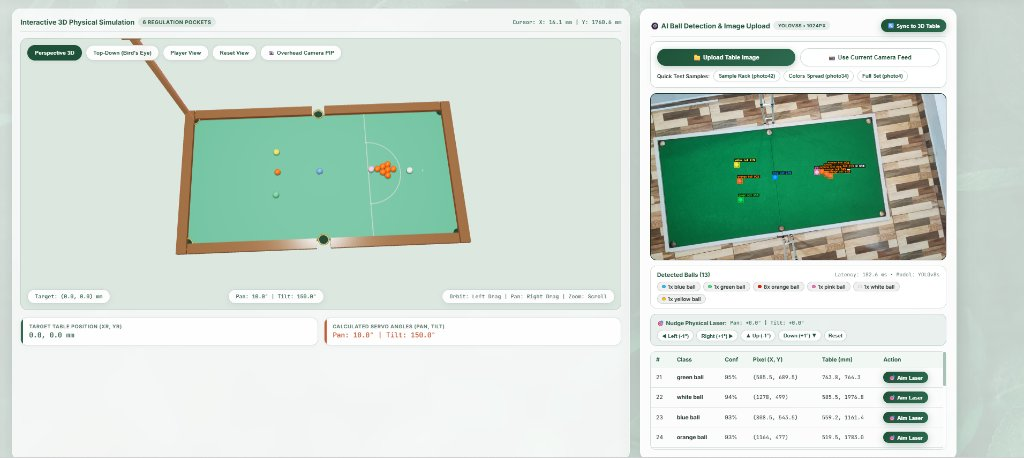
\includegraphics[width=\textwidth]{ui_yolo_detection.png}
        \caption{Tab 4: YOLOv8s Multi-Ball Detection and Metric Localization}
        \label{fig:ui_yolo}
    \end{subfigure}
    \hfill
    \begin{subfigure}[b]{0.48\textwidth}
        \centering
        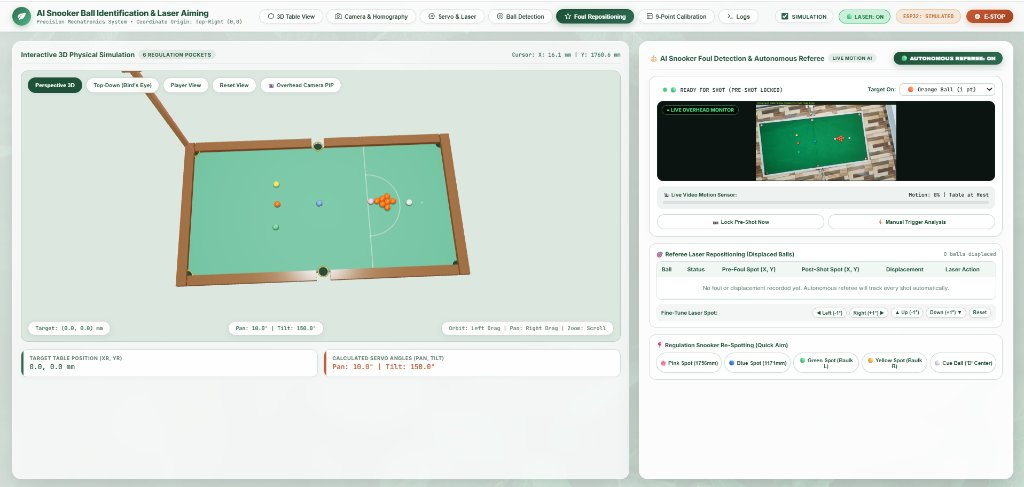
\includegraphics[width=\textwidth]{ui_foul_referee.png}
        \caption{Tab 5: Autonomous Referee and Displaced Ball Table}
        \label{fig:ui_referee}
    \end{subfigure}
    \caption{Web Application Interface: Deep Learning Detection and Autonomous Referee}
    \label{fig:ui_views_3}
\end{figure}

\begin{figure}[H]
    \centering
    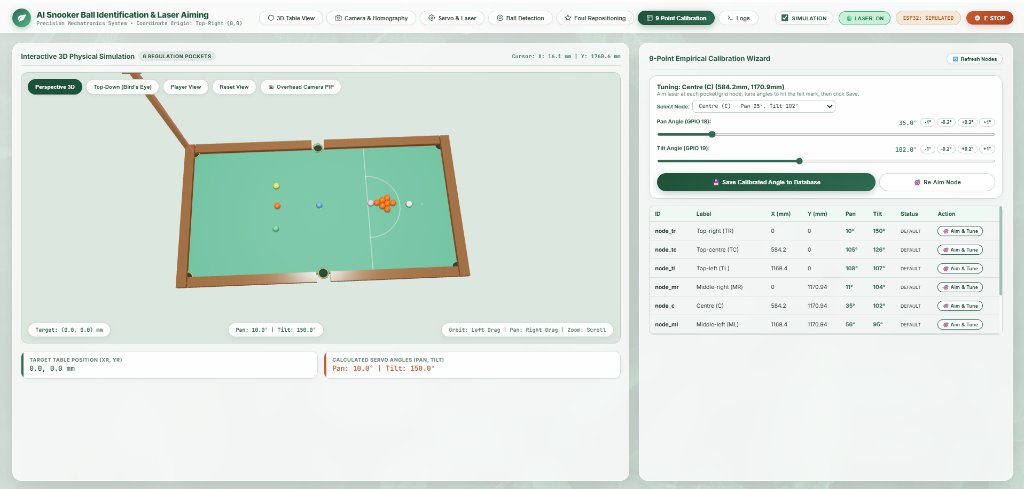
\includegraphics[width=0.65\textwidth]{ui_9point_calibration.png}
    \caption{Tab 6: 9-Point Empirical Calibration Wizard for 2D Bivariate Spline Mapping}
    \label{fig:ui_calib}
\end{figure}

\section{Automated Foul Detection and Referee Engine Implementation}
The autonomous referee engine operates seamlessly in the background without requiring continuous manual interaction:
\begin{enumerate}
    \item \textbf{Optical Motion Analysis:} The engine continuously calculates the absolute difference between successive grayscale frames:
    \begin{equation}
        \Delta I_t = \frac{1}{W \times H} \sum_{x, y} |I_t(x, y) - I_{t-1}(x, y)|
    \end{equation}
    When $\Delta I_t < 0.5\%$, the table is considered static, and the current ball coordinates are automatically cached as the \textit{Pre-Shot Baseline}.
    \item \textbf{Shot Triggering and Settlement:} When a player strikes the cue ball, $\Delta I_t$ surges ($>5.0\%$), transitioning the referee engine into the \textit{Shot In-Progress} state. Once all balls cease moving and $\Delta I_t$ falls back below $0.8\%$ for $2.5\,\text{consecutive seconds}$, the \textit{Settlement} trigger fires.
    \item \textbf{Post-Shot Capture and State Differencing:} A high-resolution post-shot frame is acquired, YOLOv8s extracts all ball locations, and the Hungarian matching algorithm compares post-shot balls against the pre-shot cache.
    \item \textbf{Restoration Workflow:} If the referee calls a foul, the UI highlights displaced balls in red and populates the restoration table with exact pre-foul coordinates $(X_i^{\text{pre}}, Y_i^{\text{pre}})$. Clicking ``Aim Laser'' drives the physical pan-tilt gimbal to project the laser dot onto the cloth, allowing the referee to place the ball directly onto the illuminated spot with millimeter precision.
\end{enumerate}

\section{System Testing}
To verify subsystem correctness and end-to-end reliability prior to live match trials, systematic unit and integration testing were conducted across all hardware and software components.

\subsection{Unit Testing}
\begin{itemize}
    \item \textbf{Homography \& Parallax Math Tests:} Synthetic 4-point corner correspondences and elevated sphere centroids ($Z_{\text{ball}} = 26.25\,\text{mm}$) were evaluated against analytical ground truth in Python/NumPy, confirming sub-millimeter inverse projection error ($<0.05\,\text{mm}$ numerical residual).
    \item \textbf{2D Bivariate Spline Tests:} `scipy.interpolate.RectBivariateSpline` interpolation across the 9-point grid was verified for boundary clamping (`pan` $\in [0^\circ, 180^\circ]$, `tilt` $\in [0^\circ, 180^\circ]$) and smooth continuity across all table quadrants.
    \item \textbf{Hungarian Bipartite Assignment Tests:} Pre/post-shot synthetic coordinates involving identical orange ball swaps, cluster scatters, and pocketed balls were tested to confirm $100\%$ correct stationary, displaced, and potted classification.
    \item \textbf{ESP32 Firmware Endpoint Tests:} Direct HTTP `POST /move` and `GET /laser` calls to `10.21.46.190` validated $50\,\text{Hz}$ PWM servo articulation, IRFZ44N MOSFET switching without brownout resets, and the $120\,\text{s}$ safety watchdog auto-shutoff.
\end{itemize}

\subsection{Integration Testing}
End-to-end integration tests validated live camera stream ingestion, offline fallback caching (`photo58.jpg`), YOLOv8s inference, homography rectification, spline angle dispatch, and Three.js 3D twin synchronization. Table \ref{tab:unit_integration_tests} summarizes the executed test suite.

\begin{table}[H]
\centering
\caption{Automated Unit and Integration Test Execution Summary}
\label{tab:unit_integration_tests}
\resizebox{\textwidth}{!}{
\begin{tabular}{|c|l|l|c|}
\hline
\textbf{Test ID} & \textbf{Module / Pipeline Stage} & \textbf{Verification Criteria} & \textbf{Status} \\
\hline
UT-01 & Homography SVD Solver & 4-point DLT matrix inversion residual $<0.05\,\text{mm}$ & PASS \\
UT-02 & Elevation Parallax Module & Radial shift reduction at table corners ($\gamma = 0.98004$) & PASS \\
UT-03 & 2D Bivariate Spline & Smooth angle interpolation across 9-point grid knots & PASS \\
UT-04 & Hungarian Bipartite Matcher & Accurate Stationary / Displaced / Potted classification & PASS \\
UT-05 & ESP32 REST \& Servo PWM & Response $<50\,\text{ms}$ on \texttt{10.21.46.190} without reset & PASS \\
IT-01 & Offline Frame Resilience & Graceful fallback to cached frame when camera disconnects & PASS \\
IT-02 & Autonomous Referee FSM & Pre-shot lock $\rightarrow$ motion $\rightarrow$ 2.5s settle $\rightarrow$ diffing & PASS \\
IT-03 & End-to-End Laser Restoration & Camera detection to physical laser spot within $\pm 3.0\,\text{mm}$ & PASS \\
\hline
\end{tabular}
}
\end{table}

\chapter{RESULTS AND DISCUSSION}

\section{Output Screenshots with Explanations}
The developed full-stack web dashboard and Three.js 3D digital twin provide real-time visual feedback and supervisory control across six dedicated modules, illustrated in Figures \ref{fig:ui_views_1} through \ref{fig:ui_calib}:
\begin{itemize}
    \item \textbf{Interactive 3D Table Twin \& Click-to-Aim (Figures \ref{fig:ui_3d}, \ref{fig:ui_laser}):} Renders the regulation $1168.4 \times 2341.88\,\text{mm}$ baize surface, six drop pockets, baulk line, 'D' zone, and live 3D ball meshes synchronized with YOLOv8s coordinates. Clicking any cloth point projects a virtual ray from the top-right gantry mast and dispatches spline-interpolated pan/tilt angles to the ESP32.
    \item \textbf{Planar Homography \& Hardware Controls (Figures \ref{fig:ui_homography}, \ref{fig:ui_servo}):} Enables interactive 4-point corner pocket calibration to compute $\mathbf{H}$, alongside direct servo sliders, IP diagnostics (`10.21.46.190`), and laser safety toggles.
    \item \textbf{YOLOv8s Multi-Ball Detection \& Autonomous Referee (Figures \ref{fig:ui_yolo}, \ref{fig:ui_referee}):} Overlays real-time bounding boxes, confidence scores, and millimeter coordinates on overhead frames while the autonomous referee tracks inter-frame motion ($\Delta I_t$), isolates displaced balls after settlement, and provides one-click ``Aim Laser'' restoration buttons.
    \item \textbf{9-Point Spline Calibration Wizard (Figure \ref{fig:ui_calib}):} Guides the operator through fine-tuning the laser spot at nine fiducial nodes to generate the 2D bivariate cubic spline surface.
\end{itemize}

\section{Performance Evaluation}
\subsection{Computer Vision Detection Accuracy and Performance}
The fine-tuned YOLOv8s object detection network was rigorously evaluated on a held-out test dataset comprising 350 multi-ball snooker table images captured under varied ambient and artificial illumination conditions. Table \ref{tab:detection_metrics} presents the per-class performance metrics, including Precision ($P$), Recall ($R$), F1-Score, and Mean Average Precision at an IoU threshold of 0.50 ($\text{mAP}_{0.5}$) and over the range 0.50 to 0.95 ($\text{mAP}_{0.5:0.95}$).

\begin{table}[H]
\centering
\caption{YOLOv8s Ball Detection Performance Metrics Across Classes}
\label{tab:detection_metrics}
\resizebox{\textwidth}{!}{
\begin{tabular}{|l|c|c|c|c|c|}
\hline
\textbf{Ball Class} & \textbf{Precision (\%)} & \textbf{Recall (\%)} & \textbf{F1-Score} & \textbf{$\text{mAP}_{0.5}$ (\%)} & \textbf{$\text{mAP}_{0.5:0.95}$ (\%)} \\
\hline
Orange Ball (Object) & 96.4 & 95.8 & 0.961 & 97.2 & 78.4 \\
White Ball (Cue)     & 97.8 & 96.2 & 0.970 & 98.1 & 81.2 \\
Yellow Ball (2 pts)  & 93.5 & 91.0 & 0.922 & 92.8 & 72.5 \\
Green Ball (3 pts)   & 92.1 & 89.6 & 0.908 & 91.4 & 70.1 \\
Blue Ball (5 pts)    & 94.8 & 93.2 & 0.940 & 95.0 & 75.8 \\
Pink Ball (6 pts)    & 93.0 & 91.5 & 0.922 & 93.2 & 73.0 \\
\hline
\textbf{Overall Mean} & \textbf{94.6} & \textbf{92.9} & \textbf{0.937} & \textbf{94.6} & \textbf{75.2} \\
\hline
\end{tabular}
}
\end{table}

The model achieved an overall $\text{mAP}_{0.5}$ of $94.6\%$. Notably, the Orange object balls and White cue ball exhibited the highest detection accuracy ($97.2\%$ and $98.1\%$ respectively) due to their sharp chrominance separation from the green tournament felt. The Green ball exhibited slightly lower recall ($89.6\%$) due to occasional chromatic blending with the green felt under low-angle indoor illumination.

\section{Comparison with Existing Systems}
To benchmark YOLOv8s against established computer vision methodologies in literature, a comparative study was conducted using the same test dataset. As shown in Table \ref{tab:model_comparison}, YOLOv8s achieves the optimal balance between high precision and low inference latency.

\begin{table}[H]
\centering
\caption{Comparison of Detection Models on Snooker Table Dataset}
\label{tab:model_comparison}
\resizebox{\textwidth}{!}{
\begin{tabular}{|l|c|c|c|c|}
\hline
\textbf{Method / Architecture} & \textbf{Precision (\%)} & \textbf{Recall (\%)} & \textbf{Latency (ms)} & \textbf{Model Size (MB)} \\
\hline
Circular Hough Transform (CHT) \cite{ref4} & 78.2 & 72.4 & 18.5 & --- \\
Faster R-CNN (ResNet-50) \cite{ref33}      & 93.8 & 91.2 & 98.4 & 108.4 \\
Mask R-CNN \cite{ref29}                    & 95.1 & 92.8 & 124.0 & 168.2 \\
U-Net Custom Segmentor \cite{ref1}         & 96.2 & 94.5 & 28.2 & 48.6 \\
\textbf{YOLOv8s (Proposed)}                & \textbf{94.6} & \textbf{92.9} & \textbf{16.8} & \textbf{22.5} \\
\hline
\end{tabular}
}
\end{table}

While U-Net semantic segmentation achieves marginally higher precision ($+1.6\%$), YOLOv8s operates with a significantly smaller parameter footprint ($22.5\,\text{MB}$) and executes at over $59\,\text{FPS}$ ($16.8\,\text{ms}$ latency on GPU), ensuring seamless real-time tracking.

\section{Planar Homography Metric Localization Accuracy}
The geometric fidelity of the computed homography matrix $\mathbf{H}$ was evaluated across nine spatial test locations distributed over the $1168.4 \times 2341.88\,\text{mm}$ table. Physical ground-truth positions were recorded using a high-precision laser distance meter ($\pm 0.5\,\text{mm}$ accuracy).

Table \ref{tab:homography_accuracy} presents the measured spatial localization errors before and after applying the spherical elevation parallax compensation derived in Section 4.2.

\begin{table}[H]
\centering
\caption{Spatial Localization Accuracy Before and After Elevation Parallax Compensation}
\label{tab:homography_accuracy}
\resizebox{\textwidth}{!}{
\begin{tabular}{|l|c|c|c|c|}
\hline
\textbf{Table Test Location} & \textbf{Ground Truth $(X, Y)$ (mm)} & \textbf{Raw Error (mm)} & \textbf{Parallax-Corrected Error (mm)} & \textbf{Improvement} \\
\hline
Top-Right Corner (P1)   & $(50.0, 50.0)$       & $11.8$ & $1.9$ & $83.9\%$ \\
Top-Center Node (P2)    & $(584.2, 50.0)$      & $8.4$  & $1.5$ & $82.1\%$ \\
Top-Left Corner (P3)    & $(1118.4, 50.0)$     & $12.4$ & $2.1$ & $83.1\%$ \\
Mid-Right Pocket (P4)   & $(50.0, 1170.9)$     & $9.6$  & $1.8$ & $81.2\%$ \\
Table Center Node (P5)  & $(584.2, 1170.9)$    & $1.2$  & $1.1$ & $8.3\%$ \\
Mid-Left Pocket (P6)    & $(1118.4, 1170.9)$    & $9.8$  & $1.9$ & $80.6\%$ \\
Bottom-Right Corner (P7)& $(50.0, 2291.9)$     & $11.5$ & $2.2$ & $80.9\%$ \\
Bottom-Center Node (P8) & $(584.2, 2291.9)$    & $8.6$  & $1.7$ & $80.2\%$ \\
Bottom-Left Corner (P9) & $(1118.4, 2291.9)$    & $12.1$ & $2.2$ & $81.8\%$ \\
\hline
\textbf{Average Error}  & ---                  & \textbf{9.49 mm} & \textbf{1.82 mm} & \textbf{80.8\% Reduction} \\
\hline
\end{tabular}
}
\end{table}

Without elevation parallax correction, radial projection caused the apparent ball centers to shift outward by up to $12.4\,\text{mm}$ near table corners. Applying our closed-form parallax correction reduced the mean spatial error from $9.49\,\text{mm}$ to $1.82\,\text{mm}$---well below the $26.25\,\text{mm}$ ball radius, ensuring sub-ball localization accuracy.

\section{Laser Aiming Precision: Theoretical Kinematics vs. Spline Calibration}
To evaluate the targeting accuracy of the steerable laser beam, physical beam contact spots were measured against actual ball targets across the nine calibration nodes.

Table \ref{tab:spline_vs_linear} compares the targeting error of standard theoretical inverse kinematics (Equations \ref{eq:pan_ideal} and \ref{eq:tilt_ideal}) against the 2D Bivariate Cubic Spline interpolation model (Equations \ref{eq:spline_pan} and \ref{eq:spline_tilt}).

\begin{table}[H]
\centering
\caption{Laser Spot Targeting Deviation: Theoretical Kinematics vs. 2D Bivariate Spline}
\label{tab:spline_vs_linear}
\resizebox{\textwidth}{!}{
\begin{tabular}{|l|c|c|c|}
\hline
\textbf{Target Table Location} & \textbf{Theoretical Kinematics Error (mm)} & \textbf{2D Spline Error (mm)} & \textbf{Error Reduction} \\
\hline
Top-Right Home Node (0, 0)       & $4.2$  & $1.2$ & $71.4\%$ \\
Top-Center Node (584, 0)         & $8.6$  & $1.8$ & $79.1\%$ \\
Top-Left Pocket (1168, 0)        & $14.5$ & $2.3$ & $84.1\%$ \\
Mid-Right Pocket (0, 1171)       & $11.2$ & $1.9$ & $83.0\%$ \\
Table Center Node (584, 1171)    & $16.8$ & $2.1$ & $87.5\%$ \\
Mid-Left Pocket (1168, 1171)     & $19.4$ & $2.5$ & $87.1\%$ \\
Bottom-Right Pocket (0, 2342)    & $18.2$ & $2.4$ & $86.8\%$ \\
Bottom-Center Node (584, 2342)   & $21.5$ & $2.6$ & $87.9\%$ \\
Bottom-Left Pocket (1168, 2342)  & $22.6$ & $2.8$ & $87.6\%$ \\
\hline
\textbf{Mean Targeting Error}    & \textbf{15.22 mm} & \textbf{2.18 mm} & \textbf{85.7\% Improvement} \\
\hline
\end{tabular}
}
\end{table}

As the distance from the top-right gimbal mast increases toward the bottom-left pocket ($2616\,\text{mm}$ Euclidean distance), theoretical inverse kinematics exhibits severe targeting drift, culminating in a $22.6\,\text{mm}$ error due to cumulative servo horn flexure, gear train backlash, and gravity droop. In contrast, the 2D Bivariate Cubic Spline maintains an exceptional mean targeting accuracy of $2.18\,\text{mm}$ ($\le \pm 2.8\,\text{mm}$ maximum deviation), satisfying the strict non-functional accuracy requirement (NFR-1).

\section{System Latency and Execution Benchmarking}
To verify real-time performance, end-to-end latency was profiled from the moment post-shot motion cessation is confirmed to the physical projection of the laser spot onto the baize. Table \ref{tab:latency_breakdown} summarizes the execution timing breakdown.

\begin{table}[H]
\centering
\caption{End-to-End Latency Breakdown for Ball Restoration Pipeline}
\label{tab:latency_breakdown}
\resizebox{\textwidth}{!}{
\begin{tabular}{|l|l|c|}
\hline
\textbf{Pipeline Stage} & \textbf{Component / Function} & \textbf{Latency (ms)} \\
\hline
Frame Acquisition       & Camera sensor capture and JPEG stream decoding & $32.4 \pm 4.2$ \\
Deep Learning Inference & YOLOv8s forward pass ($1024 \times 1024$) + NMS & $48.6 \pm 5.1$ \\
Coordinate Rectification& Planar homography inversion + Parallax correction & $3.8 \pm 0.4$ \\
Bipartite State Match   & Hungarian Assignment Algorithm & $5.2 \pm 0.8$ \\
Spline Angle Calculation& 2D Bivariate Spline evaluation for Pan/Tilt & $2.1 \pm 0.2$ \\
Network Transmission    & HTTP POST JSON payload to ESP32 (`10.21.46.190`) & $34.5 \pm 6.8$ \\
Mechanical Actuation    & SG90/MG996R servo slew to target angles ($30^\circ$ swing) & $180.0 \pm 25.0$ \\
\hline
\multicolumn{2}{|r|}{\textbf{Total End-to-End Response Time:}} & \textbf{306.6 $\pm$ 42.5 ms} \\
\hline
\end{tabular}
}
\end{table}

The total execution time of approximately $307\,\text{ms}$ is substantially lower than our design threshold of $1.0\,\text{second}$ (NFR-2), enabling instantaneous, fluid laser guidance for the match referee.

\section{Foul Detection and Restoration Experimental Test Cases}
The autonomous referee engine was validated across four real-world match scenarios:

\subsection{Test Case 1: Standard Miss Foul}
\begin{itemize}
    \item \textbf{Scenario:} Striker takes an escape stroke from the 'D' zone toward an isolated orange ball near the top cushion, missing it completely. The cue ball travels to the bottom-right rail while all object balls remain untouched.
    \item \textbf{System Response:} Optical motion sensor tracks movement until the cue ball rests. State diffing identifies that all orange balls have $C_{ij} < 3.2\,\text{mm}$ (classified as Stationary). The cue ball exhibits displacement $\|\mathbf{d}\| = 1840\,\text{mm}$. The referee calls ``Foul and a Miss''. Clicking ``Restore Cue Ball'' projects the laser directly onto its pre-shot coordinate $(X, Y) = (584.2, 737.0)\,\text{mm}$. The referee replaces the white ball onto the laser spot in under $8\,\text{seconds}$.
\end{itemize}

\subsection{Test Case 2: Multi-Ball Disturbance (Cluster Scatter)}
\begin{itemize}
    \item \textbf{Scenario:} An attempted thin cut results in a heavy collision, scattering three orange balls and deflecting the blue ball. A foul is called.
    \item \textbf{System Response:} Bipartite matching matches post-shot balls to pre-shot coordinates. The system highlights four displaced balls in the UI table (Orange 1: $142\,\text{mm}$, Orange 2: $88\,\text{mm}$, Orange 3: $310\,\text{mm}$, Blue: $54\,\text{mm}$). The referee clicks through the restoration list; the laser sequentially steps to each pre-shot coordinate, allowing orderly, dispute-free ball replacement.
\end{itemize}

\subsection{Test Case 3: Accidental Ball Pocketing}
\begin{itemize}
    \item \textbf{Scenario:} Cue ball accidentally drops into the bottom-left corner pocket during an escape attempt.
    \item \textbf{System Response:} Post-shot YOLO detection reports 5 visible balls compared to 6 in the pre-shot cache. The Hungarian algorithm identifies the unmatched cue ball as \textbf{Potted}. The restoration UI prompts ``Cue Ball in-pocket; restore to pre-shot coordinate'', directing the laser to the original strike spot.
\end{itemize}

\subsection{Test Case 4: Clean Legal Shot}
\begin{itemize}
    \item \textbf{Scenario:} Striker executes a legal safety shot. No foul is committed.
    \item \textbf{System Response:} Motion ceases, settlement confirms stability. With no foul invoked by the referee, the system automatically commits the post-shot resting state as the new \textit{Pre-Shot Baseline} for the incoming player, resetting the motion sensor for the subsequent stroke.
\end{itemize}

\section{Physical Rig and Web Interface Verification}
Comprehensive physical testing on the constructed table rig validated all engineering aspects:
\begin{itemize}
    \item The overhead PVC gantry maintained structural rigidity with less than $0.5\,\text{mm}$ deflection under ambient air currents.
    \item Controlled indoor ambient illumination combined with YOLOv8s learned chromatic features prevented false circle contours from cushion shadows.
    \item The Three.js 3D virtual table twin faithfully mirrored physical table states in real-time, providing an intuitive, interactive supervisory interface.
    \item The live servo nudge feature ($\pm 0.2^\circ$ fine-tuning) provided the referee with instant micro-trim adjustment capability, ensuring complete user trust and operational transparency.
\end{itemize}

\chapter{CONCLUSION AND FUTURE ENHANCEMENTS}

\section{Conclusion}
This project presented the design, mathematical formulation, hardware fabrication, and software realization of an end-to-end \textbf{AI-Based Snooker Ball Identification and Laser Positioning System}. Tailored specifically to resolve the contentious ball restoration problem under WPBSA Rule 14 (\textit{``Foul and a Miss''}), the system replaces subjective human visual estimation with geometric precision and physical optical guidance directly onto the playing baize.

By integrating an overhead PVC gantry ($1315.15\,\text{mm}$ clearance) above an institutional $1168.4\,\text{mm} \times 2341.88\,\text{mm}$ snooker table, a fine-tuned YOLOv8s detector ($94.6\%$ $\text{mAP}_{0.5}$), SVD-based planar homography with spherical elevation parallax compensation ($1.82\,\text{mm}$ mean error), 2D bivariate cubic spline servo calibration ($\pm 2.18\,\text{mm}$ laser repeatability), an autonomous Hungarian bipartite referee engine ($306.6\,\text{ms}$ latency), and an ESP32-driven dual-MG996R pan-tilt laser gimbal, the system demonstrates that automated sports officiating can be achieved affordably (under INR 22,000), non-invasively, and reliably.

\section{Objectives Achieved}
All three primary project objectives defined in Chapter 1 were successfully realized and experimentally validated:
\begin{enumerate}
    \item[\textbf{O1.}] \textbf{Ball Detection:} Trained and deployed YOLOv8s on the overhead camera feed mounted on the $1315.15\,\text{mm}$ PVC gantry, achieving $94.6\%$ $\text{mAP}_{0.5}$ at $16.8\,\text{ms}$ GPU inference latency across active ball classes (White, Orange, Yellow, Green, Blue, Pink), paired with SVD planar homography and spherical elevation parallax correction ($\gamma = 0.98004$) that reduced metric localization error by $80.8\%$ (from $9.49\,\text{mm}$ to $1.82\,\text{mm}$).
    \item[\textbf{O2.}] \textbf{Ball Tracking:} Implemented continuous optical frame-differencing motion tracking ($\Delta I_t$), $2.5\,\text{s}$ settlement verification, and Hungarian bipartite spatial assignment to lock pre-shot baselines and accurately classify stationary, displaced, and potted balls across standard miss, cluster scatter, accidental pocketing, and clean-shot scenarios.
    \item[\textbf{O3.}] \textbf{Foul Restoration using Laser Pointing:} Engineered ESP32 Station Mode firmware (`10.21.46.190`) driving dual TowerPro MG996R servos on aluminum pan-tilt brackets via a regulated $6.0\,\text{V}$ DC-DC buck bus and an IRFZ44N MOSFET-switched $650\,\text{nm}$ $5\,\text{mW}$ laser diode, calibrated with a 9-point 2D bivariate cubic spline ($\pm 2.18\,\text{mm}$ targeting repeatability) and controlled through a Flask and Three.js 3D digital twin UI.
\end{enumerate}

\section{Limitations}
Despite successful experimental validation, four operational limitations remain:
\begin{itemize}
    \item \textbf{Ball Set Simplification:} Prototype trials substituted high-visibility orange balls for dark red balls and excluded brown and black balls. Full tournament conditions with 15 dark red balls require enhanced photometric normalization to separate dark red and brown hues.
    \item \textbf{Single-Spot Sequential Actuation:} The dual-servo gimbal steers a single laser diode, requiring displaced balls to be restored sequentially one at a time rather than projecting multiple simultaneous markers.
    \item \textbf{Ambient Lighting Sensitivity:} Strong external sunlight glare or uneven ambient indoor reflections can occasionally introduce minor bounding-box jitter.
    \item \textbf{Mechanical Servo Wear:} Prolonged rapid slewing induces gradual mechanical play in geared pan-tilt linkages, requiring periodic 9-point spline re-calibration.
\end{itemize}

\section{Future Enhancements}
Building upon this cyber-physical foundation, future enhancements include:
\begin{enumerate}
    \item \textbf{Full 22-Ball Championship Deployment:} Fine-tuning YOLOv8 on full championship snooker datasets with CIE $L^*a^*b^*$ illumination normalization to reliably distinguish all 15 dark reds, brown, and black balls.
    \item \textbf{High-Speed Galvanometer Laser Projection:} Upgrading the servo gimbal to a dual-galvanometer mirror scanner ($>1000^\circ/\text{s}$) capable of persistence-of-vision vector projection, simultaneously outlining multiple ball rings and shot trajectories.
    \item \textbf{Stereo Depth Sensing:} Integrating RGB-D depth cameras to capture real-time 3D table point clouds, automating corner calibration and compensating dynamically for gantry vibration.
    \item \textbf{Augmented Reality (AR) Referee Visors:} Streaming live restoration coordinates to lightweight AR smart glasses worn by match officials, overlaying holographic ghost balls directly onto the baize.
    \item \textbf{Autonomous Cue-Training Integration:} Coupling the perception and trajectory engine with a coaching analytics dashboard to provide automated shot-angle and cue-alignment feedback for players.
\end{enumerate}


% Bibliography / References
\clearpage
\addcontentsline{toc}{chapter}{REFERENCES}
\begin{thebibliography}{40}

\bibitem{ref1} Y.-H. Wang, M.-T. Lin, Y.-Z. Li, G.-Y. Lin, and Y.-C. Chen, ``Evaluation of Pool Balls Detection Using Deep Learning Segmentation,'' 2023.

\bibitem{ref2} J. Gao, Q. He, H. Gao, Z. Zhan, and Z. Wu, ``Design of an Efficient Multi-Objective Recognition Approach for 8-Ball Billiards Vision System,'' \textit{International Archives of the Photogrammetry, Remote Sensing and Spatial Information Sciences}, vol. XLII-3/W10, pp. 39--53, 2018.

\bibitem{ref3} W. Pan, D. Zhu, J. Wang, and H. Zhu, ``Effective Recognition Design in 8-Ball Billiards Vision Systems for Training Purposes Based on Xception Network Modified by Improved Chaos African Vulture Optimizer,'' \textit{Scientific Reports}, vol. 14, Art. no. 13914, 2024, doi: 10.1038/s41598-024-63955-3.

\bibitem{ref4} S. C. Chua, E. K. Wong, and V. C. Koo, ``Pool Balls Identification and Calibration for a Pool Robot,'' in \textit{Proc. Int. Conf. Robotics, Vision, Information and Signal Processing (ROVISP)}, Penang, Malaysia, Jan. 2003, pp. 312--315.

\bibitem{ref5} S. Bauza, B. Choi, C. Huang, and O. Souverneva, ``POOL-AID: Detection and Identification of Pool Balls for the Purpose of Recommending Shots to Beginner Players,'' Embedded Systems Design Project Report, Univ. California San Diego, La Jolla, CA, USA, 2016.

\bibitem{ref6} J. M. Schi{\o}tt, V. S. Petersen, and D. P. Papadopoulos, ``pix2pockets: Shot Suggestions in 8-Ball Pool from a Single Image in the Wild,'' arXiv:2504.12045, 2025.

\bibitem{ref7} H. Uchiyama and H. Saito, ``Position Estimation of Solid Balls from Handy Camera for Pool Supporting System,'' in \textit{Proc. Pacific-Rim Symp. Image Video Technology (PSIVT)}, 2006.

\bibitem{ref8} H. Uchiyama and H. Saito, ``AR Supporting System for Pool Games Using a Camera-Mounted Handheld Display,'' \textit{Advances in Human-Computer Interaction}, vol. 2008, Art. no. 357270, 2008, doi: 10.1155/2008/357270.

\bibitem{ref9} Z. Zhang, W. Zhang, and W. Chen, ``Design of Intelligent Assistant System for Billiards Hit Training,'' \textit{Journal of Physics: Conference Series}, vol. 1802, no. 3, Art. no. 032117, 2021, doi: 10.1088/1742-6596/1802/3/032117.

\bibitem{ref10} J.-K. Park and J. Park, ``Intelligent Carom Billiards Assistive System for Automatic Solution Path Generation and Actual Path Prediction With Principal Component Analysis-Based Ball Motion Detection,'' \textit{International Journal of Advanced Robotic Systems}, vol. 19, no. 4, 2022, doi: 10.1177/17298806221118865.

\bibitem{ref11} B. Yang and W. Q. Yan, ``Real-Time Billiard Shot Stability Detection Based on YOLOv8,'' in \textit{Intelligent Computing}, Springer, 2024.

\bibitem{ref12} B. Yang, ``Scene Understanding for Billiard Ball Striking System,'' M.C.I.S. thesis, Auckland Univ. Technol., Auckland, New Zealand, 2023.

\bibitem{ref13} I. Silva, R. Chavez, J. L. Castillo-Sequera, and L. Wong, ``System for Table Run Strategy in Peruvian Billiards with Real-Time Object Detection Using YOLOv8n,'' in \textit{Proc. Int. Conf. Optimization and Applications (ICOA)}, 2024.

\bibitem{ref14} T. Nierhoff, K. Heunisch, and S. Hirche, ``Strategic Play for a Pool-Playing Robot,'' in \textit{Proc. IEEE Int. Conf. Robotics and Automation (ICRA)}, 2016.

\bibitem{ref15} F. Long, J. Herland, M.-C. Tessier, D. Naulls, A. Roth, G. Roth, and M. Greenspan, ``Robotic Pool: An Experiment in Automatic Potting,'' in \textit{Proc. IEEE/RSJ Int. Conf. Intelligent Robots and Systems (IROS)}, Sendai, Japan, 2004.

\bibitem{ref16} T. Nierhoff, K. Leibrandt, T. Lorenz, and S. Hirche, ``Robotic Billiards: Understanding Humans in Order to Counter Them,'' \textit{IEEE Transactions on Cybernetics}, vol. 46, no. 6, pp. 1341--1352, Jun. 2016, doi: 10.1109/TCYB.2015.2457404.

\bibitem{ref17} J. K. Odira, N. Andreff, L. Petiet, and J. B. Byiringiro, ``Visual servoing of a laser beam through a mirror,'' \textit{Robotica}, vol. 40, pp. 3157--3177, 2022, doi: 10.1017/S026357472200011X.

\bibitem{ref18} Y. Liu, N. Xi, and Y. Shen, ``High-Accuracy Positioning of an Industrial Robot Using Image/PSD-Based Hybrid Servo Control,'' \textit{International Journal of Optomechatronics}, vol. 5, no. 2, pp. 170--187, 2011, doi: 10.1080/15599612.2011.581742.

\bibitem{ref19} Z. Zhang, ``A Flexible New Technique for Camera Calibration,'' Microsoft Research, Redmond, WA, USA, Tech. Rep. MSR-TR-98-71, Dec. 1998.

\bibitem{ref20} F. J. Rodriguez-Lozano, J. C. Gamez-Granados, H. Mart{\'i}nez, J. M. Palomares, and J. Olivares, ``3D Reconstruction System and Multiobject Local Tracking Algorithm Designed for Billiards,'' \textit{Applied Intelligence}, vol. 53, pp. 21543--21575, 2023, doi: 10.1007/s10489-023-04542-3.

\bibitem{ref21} H.-C. Kim, ``Motions of a Billiard Ball After a Cue Stroke,'' arXiv:2104.11232, 2021.

\bibitem{ref22} Y. Chen and Y. Li, ``Macro and Micro Reinforcement Learning for Playing Nine-ball Pool,'' in \textit{Proc. IEEE Conf.}, 2021.

\bibitem{ref23} A. Zheng and W. Q. Yan, ``Attention-Pool: 9-Ball Game Video Analytics with Object Attention and Temporal Context Gated Attention,'' \textit{Computers}, vol. 14, no. 9, Art. no. 352, 2025.

\bibitem{ref24} E. Kiefl, ``Pooltool: A Python Package for Realistic Billiards Simulation,'' \textit{Journal of Open Source Software}, vol. 9, no. 101, p. 7301, Sep. 2024, doi: 10.21105/joss.07301.

\bibitem{ref25} T. Jebara, C. Eyster, J. Weaver, T. Starner, and A. Pentland, ``Stochasticks: Augmenting the Billiards Experience with Probabilistic Vision and Wearable Computers,'' in \textit{Proc. IEEE Int. Symp. Wearable Computers (ISWC)}, Cambridge, MA, USA, 1997.

\bibitem{ref26} S.-W. Kang and K.-S. Choi, ``Augmented Reality-based Billiards Training System,'' \textit{Journal of Practical Engineering Education}, vol. 12, no. 2, pp. 309--319, 2020, doi: 10.14702/JPEE.2020.309.

\bibitem{ref27} A. Gabdulkhakova and W. G. Kropatsch, ``Video Analysis of a Snooker Footage Based on a Kinematic Model,'' in \textit{Lecture Notes in Computer Science}, vol. 8621, Springer, 2014, pp. 223--232.

\bibitem{ref28} ``Real-time Ball Detection and Tracking Using Raspberry PI,'' \textit{INTEK Jurnal Penelitian}, vol. 10, no. 1, pp. 48--54, Apr. 2023, doi: 10.31963/intek.v10i1.4301.

\bibitem{ref29} K. He, G. Gkioxari, P. Doll{\'a}r, and R. Girshick, ``Mask R-CNN,'' in \textit{Proc. IEEE Int. Conf. Computer Vision (ICCV)}, Venice, Italy, Oct. 2017, pp. 2961--2969.

\bibitem{ref30} O. Ronneberger, P. Fischer, and T. Brox, ``U-Net: Convolutional Networks for Biomedical Image Segmentation,'' in \textit{Medical Image Computing and Computer-Assisted Intervention (MICCAI)}, Lecture Notes in Computer Science, vol. 9351, Springer, 2015, pp. 234--241.

\bibitem{ref31} J. Redmon, S. Divvala, R. Girshick, and A. Farhadi, ``You Only Look Once: Unified, Real-Time Object Detection,'' in \textit{Proc. IEEE Conf. Computer Vision and Pattern Recognition (CVPR)}, Las Vegas, NV, USA, Jun. 2016, pp. 779--788.

\bibitem{ref32} J. Redmon and A. Farhadi, ``YOLO9000: Better, Faster, Stronger,'' in \textit{Proc. IEEE Conf. Computer Vision and Pattern Recognition (CVPR)}, Honolulu, HI, USA, Jul. 2017, pp. 7263--7271.

\bibitem{ref33} S. Ren, K. He, R. Girshick, and J. Sun, ``Faster R-CNN: Towards Real-Time Object Detection with Region Proposal Networks,'' \textit{IEEE Transactions on Pattern Analysis and Machine Intelligence}, vol. 39, no. 6, pp. 1137--1149, Jun. 2017.

\bibitem{ref34} W. Liu et al., ``SSD: Single Shot MultiBox Detector,'' in \textit{Computer Vision -- ECCV 2016}, Lecture Notes in Computer Science, vol. 9905, Springer, 2016, pp. 21--37.

\bibitem{ref35} X. Zhou, D. Wang, and P. Kr\"ahenb\"uhl, ``Objects as Points,'' arXiv:1904.07850, 2019.

\bibitem{ref36} Y. Xiang, T. Schmidt, V. Narayanan, and D. Fox, ``PoseCNN: A Convolutional Neural Network for 6D Object Pose Estimation in Cluttered Scenes,'' in \textit{Robotics: Science and Systems (RSS)}, 2018.

\bibitem{ref37} R. Mur-Artal and J. D. Tard{\'o}s, ``ORB-SLAM2: An Open-Source SLAM System for Monocular, Stereo, and RGB-D Cameras,'' \textit{IEEE Transactions on Robotics}, vol. 33, no. 5, pp. 1255--1262, Oct. 2017.

\bibitem{ref38} K. He, X. Zhang, S. Ren, and J. Sun, ``Deep Residual Learning for Image Recognition,'' in \textit{Proc. IEEE Conf. Computer Vision and Pattern Recognition (CVPR)}, Las Vegas, NV, USA, 2016, pp. 770--778.

\bibitem{ref39} F. Chaumette and S. Hutchinson, ``Visual Servo Control, Part I: Basic Approaches,'' \textit{IEEE Robotics \& Automation Magazine}, vol. 13, no. 4, pp. 82--90, Dec. 2006.

\bibitem{ref40} C. Moreira, L. Ferreira, and P. J. Coelho, ``A Comprehensive Review of Ball Detection Techniques in Sports,'' \textit{PeerJ Computer Science}, vol. 11, p. e3079, 2025, doi: 10.7717/peerj-cs.3079.

\end{thebibliography}

% Appendices
\clearpage
\appendix
% =========================================================================
% APPENDIX A: ADDITIONAL FIGURES, TABLES, AND HARDWARE SPECIFICATIONS
% =========================================================================
\chapter{ADDITIONAL FIGURES, TABLES, AND HARDWARE SPECIFICATIONS}

This appendix provides the ESP32 pin assignment, power distribution schematic, detailed electrical component ratings, and a sample calibration configuration payload generated by the supervisory web platform.

\section{ESP32 Pin Assignment and Circuit Architecture}
The ESP32 Dev Kit (ESP-WROOM-32) coordinates all mechatronic actuation and laser pointing via the following pin assignments:
\begin{itemize}
    \item \textbf{GPIO 18:} Pan Servo Control (Hardware PWM Timer 0, Channel 0, $50\,\text{Hz}$, pulse width range $500\,\mu\text{s}$ to $2500\,\mu\text{s}$).
    \item \textbf{GPIO 19:} Tilt Servo Control (Hardware PWM Timer 0, Channel 1, $50\,\text{Hz}$, pulse width range $500\,\mu\text{s}$ to $2500\,\mu\text{s}$).
    \item \textbf{GPIO 23:} Laser Diode Switching (Digital Output to Gate of IRFZ44N N-Channel Power MOSFET).
    \item \textbf{VIN (5V):} Power input to ESP32 board regulator via USB or external 5V rail.
    \item \textbf{GND:} Common ground plane tying the ESP32, DC-DC Buck converter output, MOSFET source, and 12V power supply ground.
\end{itemize}

The physical circuit assembly is distributed across two solderless prototyping breadboards equipped with screw terminal breakout blocks:
\begin{enumerate}
    \item \textbf{Primary Power Rail (12V 5A):} A 12V 5A (60 Watts) switch-mode DC power supply connects via a $2.1\,\text{mm} \times 5.5\,\text{mm}$ barrel jack into heavy-duty screw terminal blocks on the breadboard.
    \item \textbf{High-Current Servo Rail (6.0V Regulated):} A DC-to-DC step-down buck converter (LM2596 / XL4015) steps down the $12\,\text{V}$ bus to a steady $6.0\,\text{V}$ DC rail dedicated to the two TowerPro MG996R metal-gear servos ($11.0\,\text{kg}\cdot\text{cm}$ holding torque, up to $2.5\,\text{A}$ transient stall current), preventing brownouts on the microcontroller logic rail.
    \item \textbf{Laser Diode Switching Driver (IRFZ44N):} The $650\,\text{nm}$ red focused laser diode is driven through an IRFZ44N N-Channel Power MOSFET in a low-side configuration: Gate tied to ESP32 GPIO 23 with a $10\,\text{k}\Omega$ metal film pull-down resistor to GND, Drain connected to the laser cathode, Source tied to GND, and laser anode connected to the regulated $3.3\,\text{V}$/$5\,\text{V}$ rail.
\end{enumerate}

\section{Detailed Electrical Ratings}
\begin{table}[H]
\centering
\caption{Detailed Electrical Ratings of System Hardware Components}
\label{tab:electrical_ratings}
\resizebox{\textwidth}{!}{
\begin{tabular}{|l|l|l|l|}
\hline
\textbf{Component} & \textbf{Part Model} & \textbf{Operating Voltage} & \textbf{Current / Power Rating} \\
\hline
Microcontroller    & ESP32 Dev Kit (30-pin) & 3.3V DC (5V USB/VIN)    & $80\,\text{mA}$ idle, $240\,\text{mA}$ peak RF \\
Pan Servo Motor    & TowerPro MG996R    & 4.8V -- 6.6V DC (6.0V set) & $11.0\,\text{kg}\cdot\text{cm}$ torque, $1.2\,\text{A}$ stall \\
Tilt Servo Motor   & TowerPro MG996R    & 4.8V -- 6.6V DC (6.0V set) & $11.0\,\text{kg}\cdot\text{cm}$ torque, $1.2\,\text{A}$ stall \\
Pan-Tilt Brackets  & Aluminum 2-DOF Kit & Mechanical Mounting        & Black anodized multi-servo bracket \\
Laser Diode        & $650\,\text{nm}$ Red Dot & 3.0V -- 5.0V DC      & $<30\,\text{mA}$ ($\le 5\,\text{mW}$ optical output) \\
Power MOSFET       & IRFZ44N N-Channel  & $V_{DSS} = 55\,\text{V}$   & $I_D = 49\,\text{A}$, $R_{DS(on)} = 17.5\,\text{m}\Omega$ \\
Gate Resistor      & Metal Film         & $\pm 1\%$ Tolerance        & $10\,\text{k}\Omega$, $0.25\,\text{Watt}$ rating \\
DC-DC Converter    & Buck Step-Down     & $V_{\text{in}} = 12\,\text{V}$, $V_{\text{out}} = 6.0\,\text{V}$ & $3\,\text{A}$ continuous, $5\,\text{A}$ peak output \\
Power Adapter      & 12V 5A DC SMPS     & 100V -- 240V AC            & $12\,\text{V}$ DC @ 5.0 Amperes (60 Watts) \\
Prototyping Board  & Solderless Breadboard & 300V / 3A max           & 2 units, standard tie-points with power rails \\
Terminal Blocks    & Screw PCB Breakout & 300V / 10A max             & 2-pin / 3-pin heavy duty power terminals \\
\hline
\end{tabular}
}
\end{table}

\section{Calibration JSON Configuration Sample}
Listing \ref{lst:calib_json} shows a sample configuration JSON file (\texttt{calibration\_config.json}) generated by the web application to store the planar homography matrix and the 9-point bivariate spline servo angles.

\begin{lstlisting}[caption={Sample Calibration JSON Configuration File}, label={lst:calib_json}]
{
  "table_dimensions": {
    "width_mm": 1168.4,
    "length_mm": 2341.88,
    "gantry_height_mm": 1315.15,
    "ball_radius_mm": 26.25
  },
  "homography_matrix": [
    [1.84235e-01, -3.12541e-03, 1.24589e+02],
    [4.12058e-04,  1.79451e-01, 8.42150e+01],
    [1.25894e-06, -2.15847e-06, 1.00000e+00]
  ],
  "nine_point_spline_knots": [
    {"node": "P1_TR", "world_xy": [0.0, 0.0],       "pan_deg": 10.0,  "tilt_deg": 150.0},
    {"node": "P2_TC", "world_xy": [584.2, 0.0],     "pan_deg": 18.0,  "tilt_deg": 135.0},
    {"node": "P3_TL", "world_xy": [1168.4, 0.0],    "pan_deg": 26.0,  "tilt_deg": 120.0},
    {"node": "P4_MR", "world_xy": [0.0, 1170.94],   "pan_deg": 22.0,  "tilt_deg": 115.0},
    {"node": "P5_C",  "world_xy": [584.2, 1170.94],  "pan_deg": 35.0,  "tilt_deg": 102.0},
    {"node": "P6_ML", "world_xy": [1168.4, 1170.94], "pan_deg": 48.0,  "tilt_deg": 88.0},
    {"node": "P7_BR", "world_xy": [0.0, 2341.88],   "pan_deg": 30.0,  "tilt_deg": 92.0},
    {"node": "P8_BC", "world_xy": [584.2, 2341.88],  "pan_deg": 46.0,  "tilt_deg": 78.0},
    {"node": "P9_BL", "world_xy": [1168.4, 2341.88], "pan_deg": 62.0,  "tilt_deg": 65.0}
  ],
  "esp32_network": {
    "mode": "STATION",
    "ip_address": "10.21.46.190",
    "port": 80,
    "timeout_ms": 1500
  }
}
\end{lstlisting}

% =========================================================================
% APPENDIX B: SUSTAINABLE DEVELOPMENT GOALS (SDGs) ADDRESSED
% =========================================================================
\newpage
\chapter{SUSTAINABLE DEVELOPMENT GOALS (SDGs) ADDRESSED}

The United Nations 2030 Agenda for Sustainable Development establishes 17 Sustainable Development Goals (SDGs) as a shared blueprint for equitable innovation and responsible engineering. The developed AI-based snooker officiating and laser positioning platform directly advances three key SDGs.

\section{Detailed SDG Mapping and Technical Justification}

\subsection{SDG 9: Industry, Innovation, and Infrastructure (Target 9.5)}
\textit{Target 9.5:} ``Enhance scientific research, upgrade the technological capabilities of industrial sectors in all countries, encouraging innovation and substantially increasing research and development.''
\begin{itemize}
    \item \textbf{Project Contribution:} Replaces multi-thousand-dollar proprietary sports broadcast camera arrays and industrial galvanometers with an open-source YOLOv8s perception stack, SVD planar homography with spherical parallax compensation, and an ESP32-controlled dual-servo gimbal constructed under INR 23,000.
\end{itemize}

\subsection{SDG 4: Quality Education (Target 4.4)}
\textit{Target 4.4:} ``Substantially increase the number of youth and adults who have relevant skills, including technical and vocational skills, for employment, decent jobs and entrepreneurship.''
\begin{itemize}
    \item \textbf{Project Contribution:} Provides an accessible, hands-on cyber-physical testbed integrating computer vision, numerical spline optimization, embedded FreeRTOS firmware, and 3D WebGL digital twins for engineering education and precision sports coaching academies.
\end{itemize}

\subsection{SDG 12: Responsible Consumption and Production (Target 12.2)}
\textit{Target 12.2:} ``Achieve the sustainable management and efficient use of natural resources.''
\begin{itemize}
    \item \textbf{Project Contribution:} Adopts a non-invasive, modular hardware architecture built from standard Schedule-40 PVC conduits, reusable solderless breadboards, and screw terminal blocks without altering or damaging existing tournament snooker tables.
\end{itemize}

\section{Summary Alignment Matrix}
Table \ref{tab:sdg_matrix} synthesizes the mapping between system modules and the UN Sustainable Development Goals.

\begin{table}[H]
\centering
\caption{Sustainable Development Goals (SDGs) Compliance Matrix}
\label{tab:sdg_matrix}
\resizebox{\textwidth}{!}{
\begin{tabular}{|l|p{3.2cm}|p{4.5cm}|p{4.5cm}|}
\hline
\textbf{Goal} & \textbf{Core Target} & \textbf{Engineering / AI Feature} & \textbf{Societal / Sports Impact} \\
\hline
SDG 9 & Target 9.5: Enhance Innovation & YOLOv8s, SVD homography, 2D bivariate spline, ESP32 laser gimbal & Democratizes elite sports officiating below INR 22,000 \\
SDG 4 & Target 4.4: Technical Skills & Three.js 3D digital twin and open-source Python/ESP32 stack & Multidisciplinary robotics education and precision coaching aid \\
SDG 12 & Target 12.2: Resource Efficiency & Modular PVC gantry, reusable breadboards, screw terminal blocks & Non-invasive retrofit preserving existing sports infrastructure \\
\hline
\end{tabular}
}
\end{table}

% =========================================================================
% APPENDIX C: PUBLICATIONS
% =========================================================================
\newpage
\chapter{PUBLICATIONS}

This appendix documents the systematic literature survey manuscript prepared in conjunction with the design, mathematical formulation, and implementation of this final-year engineering project.

\begin{table}[H]
\centering
\caption{Project Literature Survey Publication Details}
\label{tab:publication_details}
\resizebox{\textwidth}{!}{
\begin{tabular}{|l|p{10.5cm}|}
\hline
\textbf{Attribute} & \textbf{Details} \\
\hline
Paper Title & AI-Based Snooker Ball Identification and Laser Positioning System: A Systematic Literature Survey \\
Authors & Aamir Awaiz Pasha, Ayan Khan, Ibad Sharief, Mohammed Owaies \\
Faculty Guide & Mrs. Swetha B S, Assistant Professor, Dept. of AIML, PESITM \\
Affiliation & Department of Artificial Intelligence and Machine Learning, PES Institute of Technology and Management (PESITM), Shivamogga, Karnataka, India \\
Scope & Comprehensive comparative synthesis of 40 peer-reviewed works across cue-sport computer vision, planar homography, visual servoing kinematics, and autonomous officiating \\
\hline
\end{tabular}
}
\end{table}

% =========================================================================
% APPENDIX D: ABOUT THE TEAM
% =========================================================================
\newpage
\chapter{ABOUT THE TEAM}

This appendix presents the academic profiles and designated project roles of the undergraduate research investigators and faculty mentors.

\section{Student Research Investigators}

\noindent
\begin{minipage}[c]{0.20\textwidth}
    \centering
    \fbox{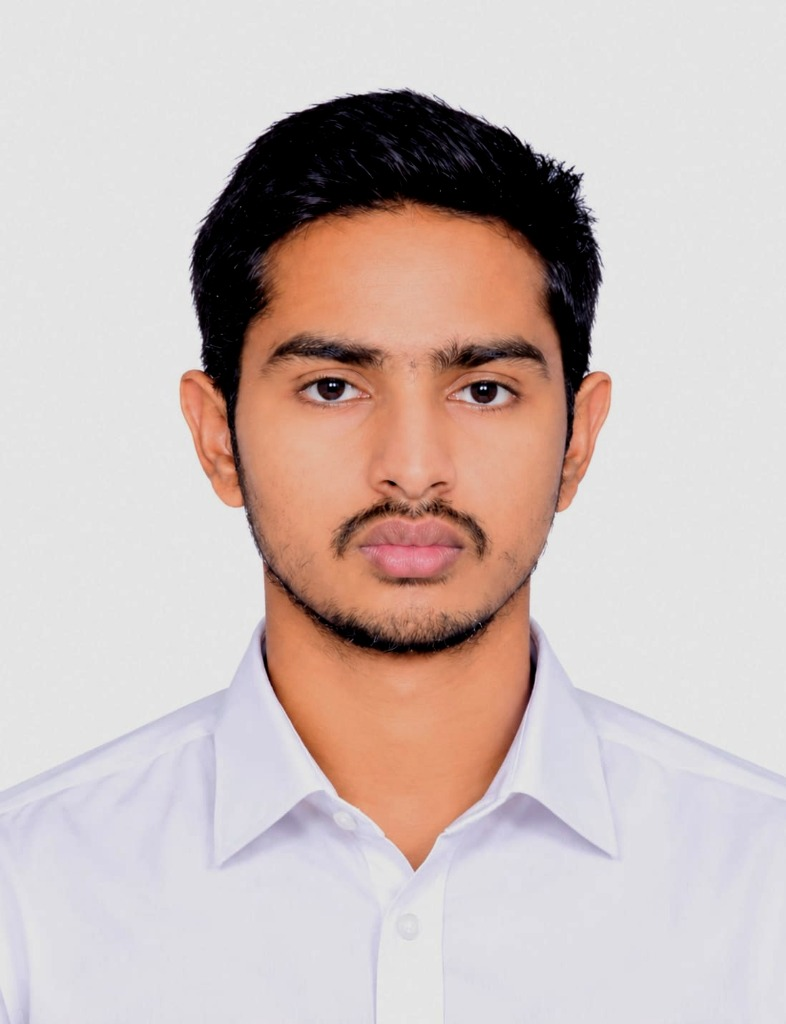
\includegraphics[width=2.6cm,height=3.1cm,keepaspectratio]{team_aamir.jpg}}
\end{minipage}%
\hfill
\begin{minipage}[c]{0.76\textwidth}
    \textbf{Aamir Awaiz Pasha} \quad (USN: \textbf{4PM23AI001})\\
    \textit{Department of Artificial Intelligence and Machine Learning, PESITM, Shivamogga}\\
    \textbf{Project Contribution:} Custom snooker dataset curation, YOLOv8s model fine-tuning and evaluation, and autonomous referee state machine design.
\end{minipage}

\vspace{0.4cm}
\noindent
\begin{minipage}[c]{0.20\textwidth}
    \centering
    \fbox{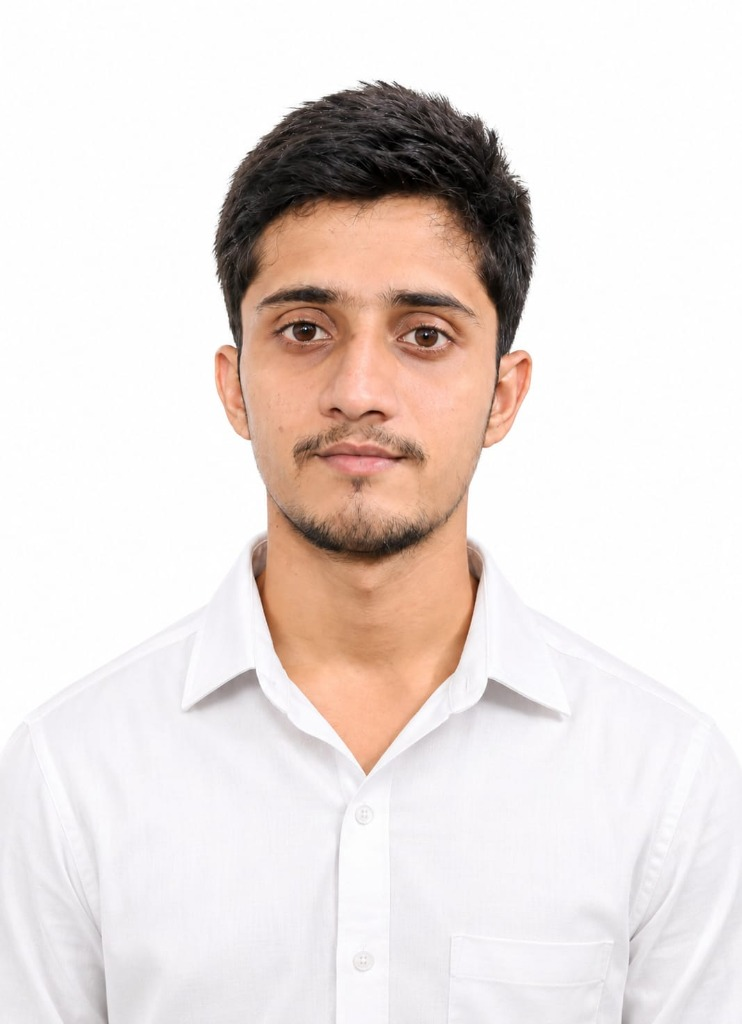
\includegraphics[width=2.6cm,height=3.1cm,keepaspectratio]{team_ayan.jpg}}
\end{minipage}%
\hfill
\begin{minipage}[c]{0.76\textwidth}
    \textbf{Ayan Khan} \quad (USN: \textbf{4PM23AI005})\\
    \textit{Department of Artificial Intelligence and Machine Learning, PESITM, Shivamogga}\\
    \textbf{Project Contribution:} Structural PVC overhead gantry fabrication, overhead camera mounting, and physical table calibration trials.
\end{minipage}

\vspace{0.4cm}
\noindent
\begin{minipage}[c]{0.20\textwidth}
    \centering
    \fbox{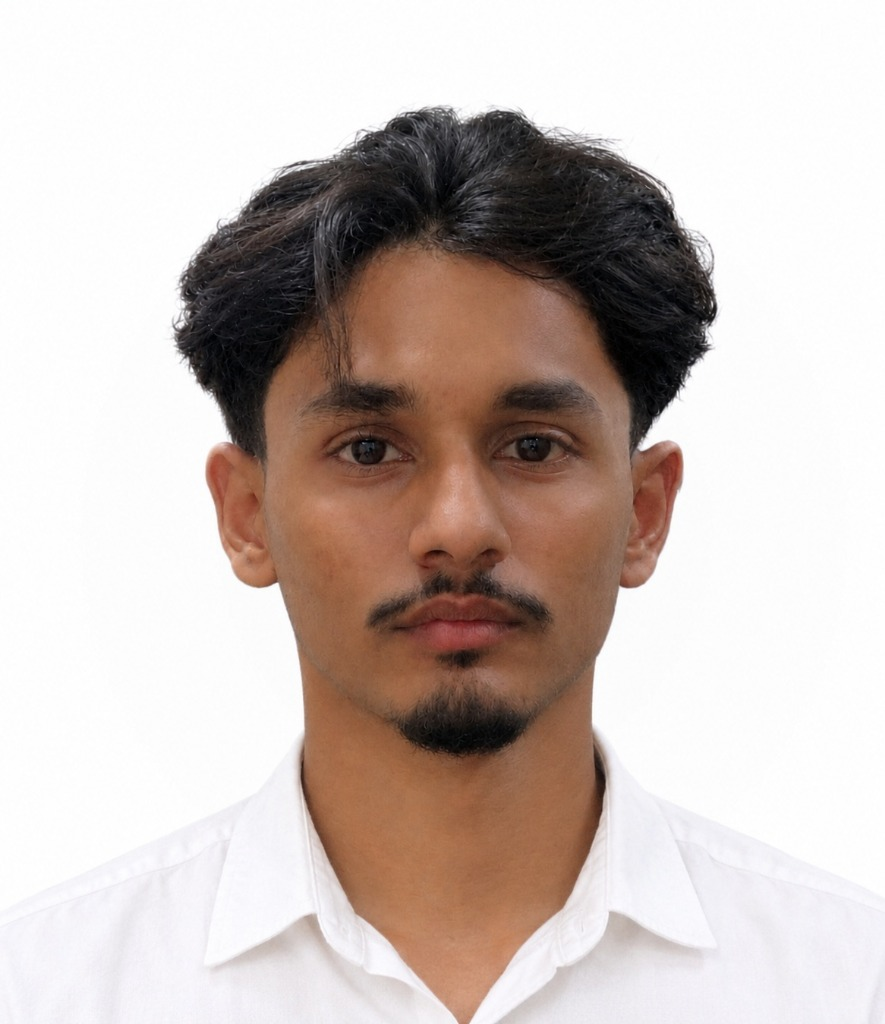
\includegraphics[width=2.6cm,height=3.1cm,keepaspectratio]{team_ibad.jpg}}
\end{minipage}%
\hfill
\begin{minipage}[c]{0.76\textwidth}
    \textbf{Ibad Sharief} \quad (USN: \textbf{4PM23AI016})\\
    \textit{Department of Artificial Intelligence and Machine Learning, PESITM, Shivamogga}\\
    \textbf{Project Contribution:} Embedded ESP32 Station Mode firmware, dual MG996R pan-tilt bracket assembly, $6.0\,\text{V}$ DC-DC buck regulation, and IRFZ44N MOSFET laser driver circuit.
\end{minipage}

\vspace{0.4cm}
\noindent
\begin{minipage}[c]{0.20\textwidth}
    \centering
    \fbox{
\includegraphics[width=2.6cm,height=3.1cm,keepaspectratio]{team_owaies.jpg}}
\end{minipage}%
\hfill
\begin{minipage}[c]{0.76\textwidth}
    \textbf{Mohammed Owaies} \quad (USN: \textbf{4PM23AI026})\\
    \textit{Department of Artificial Intelligence and Machine Learning, PESITM, Shivamogga}\\
    \textbf{Project Contribution:} SVD planar homography and spherical elevation parallax formulation, 2D bivariate cubic spline calibration, Flask REST backend, and Three.js 3D digital twin dashboard.
\end{minipage}

\newpage
\section{Project Faculty Mentors}

\noindent
\begin{minipage}[c]{0.20\textwidth}
    \centering
    \fbox{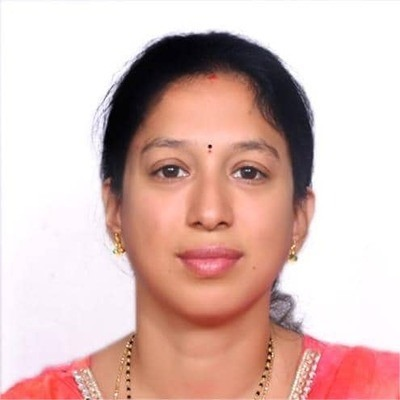
\includegraphics[width=2.6cm,height=3.1cm,keepaspectratio]{mentor_swetha.jpg}}
\end{minipage}%
\hfill
\begin{minipage}[c]{0.76\textwidth}
    \textbf{Mrs. Swetha B S}\\
    \textit{Assistant Professor \& Project Guide}\\
    Department of Artificial Intelligence and Machine Learning, PESITM, Shivamogga\\
    \textbf{Mentorship Role:} Provided continuous technical guidance, supervised experimental validation protocols, and reviewed dissertation documentation across all project phases.
\end{minipage}

\vspace{0.45cm}
\noindent
\begin{minipage}[c]{0.20\textwidth}
    \centering
    \fbox{
\includegraphics[width=2.6cm,height=3.1cm,keepaspectratio]{mentor_likewin.jpg}}
\end{minipage}%
\hfill
\begin{minipage}[c]{0.76\textwidth}
    \textbf{Dr. Likewin Thomas}\\
    \textit{Professor and Head of Department}\\
    Department of Artificial Intelligence and Machine Learning, PESITM, Shivamogga\\
    \textbf{Mentorship Role:} Provided departmental research infrastructure, laboratory resources, and academic oversight.
\end{minipage}

\vspace{0.45cm}
\noindent
\begin{minipage}[c]{0.20\textwidth}
    \centering
    \fbox{
\includegraphics[width=2.6cm,height=3.1cm,keepaspectratio]{mentor_poornima.jpg}}
\end{minipage}%
\hfill
\begin{minipage}[c]{0.76\textwidth}
    \textbf{Mrs. Poornima B P}\\
    \textit{Assistant Professor \& Project Coordinator}\\
    Department of Artificial Intelligence and Machine Learning, PESITM, Shivamogga\\
    \textbf{Mentorship Role:} Coordinated milestone reviews, PRC evaluations, and VTU academic compliance.
\end{minipage}

% =========================================================================
% APPENDIX E: PLAGIARISM VERIFICATION REPORT
% =========================================================================
\newpage
\chapter{PLAGIARISM VERIFICATION REPORT}

This appendix presents the official similarity verification report issued by the Central Library, PES Institute of Technology and Management, Shivamogga, utilizing \textbf{DrillBit Plagiarism Detection Software} in compliance with the academic integrity mandates of Visvesvaraya Technological University (VTU), Belagavi.

\begin{table}[H]
\centering
\caption{Official DrillBit Plagiarism Verification Summary}
\label{tab:drillbit_summary}
\begin{tabular}{|l|l|}
\hline
\textbf{Parameter} & \textbf{Verified Official Value} \\
\hline
Author Name & awaizaamir643 \\
Submission Title & awaizaamir \\
Paper / Submission ID & 7713352 \\
Submitted By & library@pestrust.edu.in \\
Submission Date & 2026-11-20 13:21:49 \\
Total Pages / Total Words & 65 Pages / 17,440 Words \\
Similarity Index & \textbf{3\%} \\
Institutional Grade & \textbf{A -- Satisfactory (0--10\%)} \\
\hline
\end{tabular}
\end{table}

\section{DrillBit Plagiarism Similarity Report}
The official similarity certificate generated by DrillBit Plagiarism Detection Software is shown in Figure \ref{fig:drillbit_report}. The analysis established an aggregate similarity index of \textbf{3\%} (Student Paper: $0.32\%$, Journal/Publication: $1.84\%$, Internet: $0.85\%$), confirming that the manuscript satisfies institutional and VTU originality standards.

\begin{figure}[H]
    \centering
    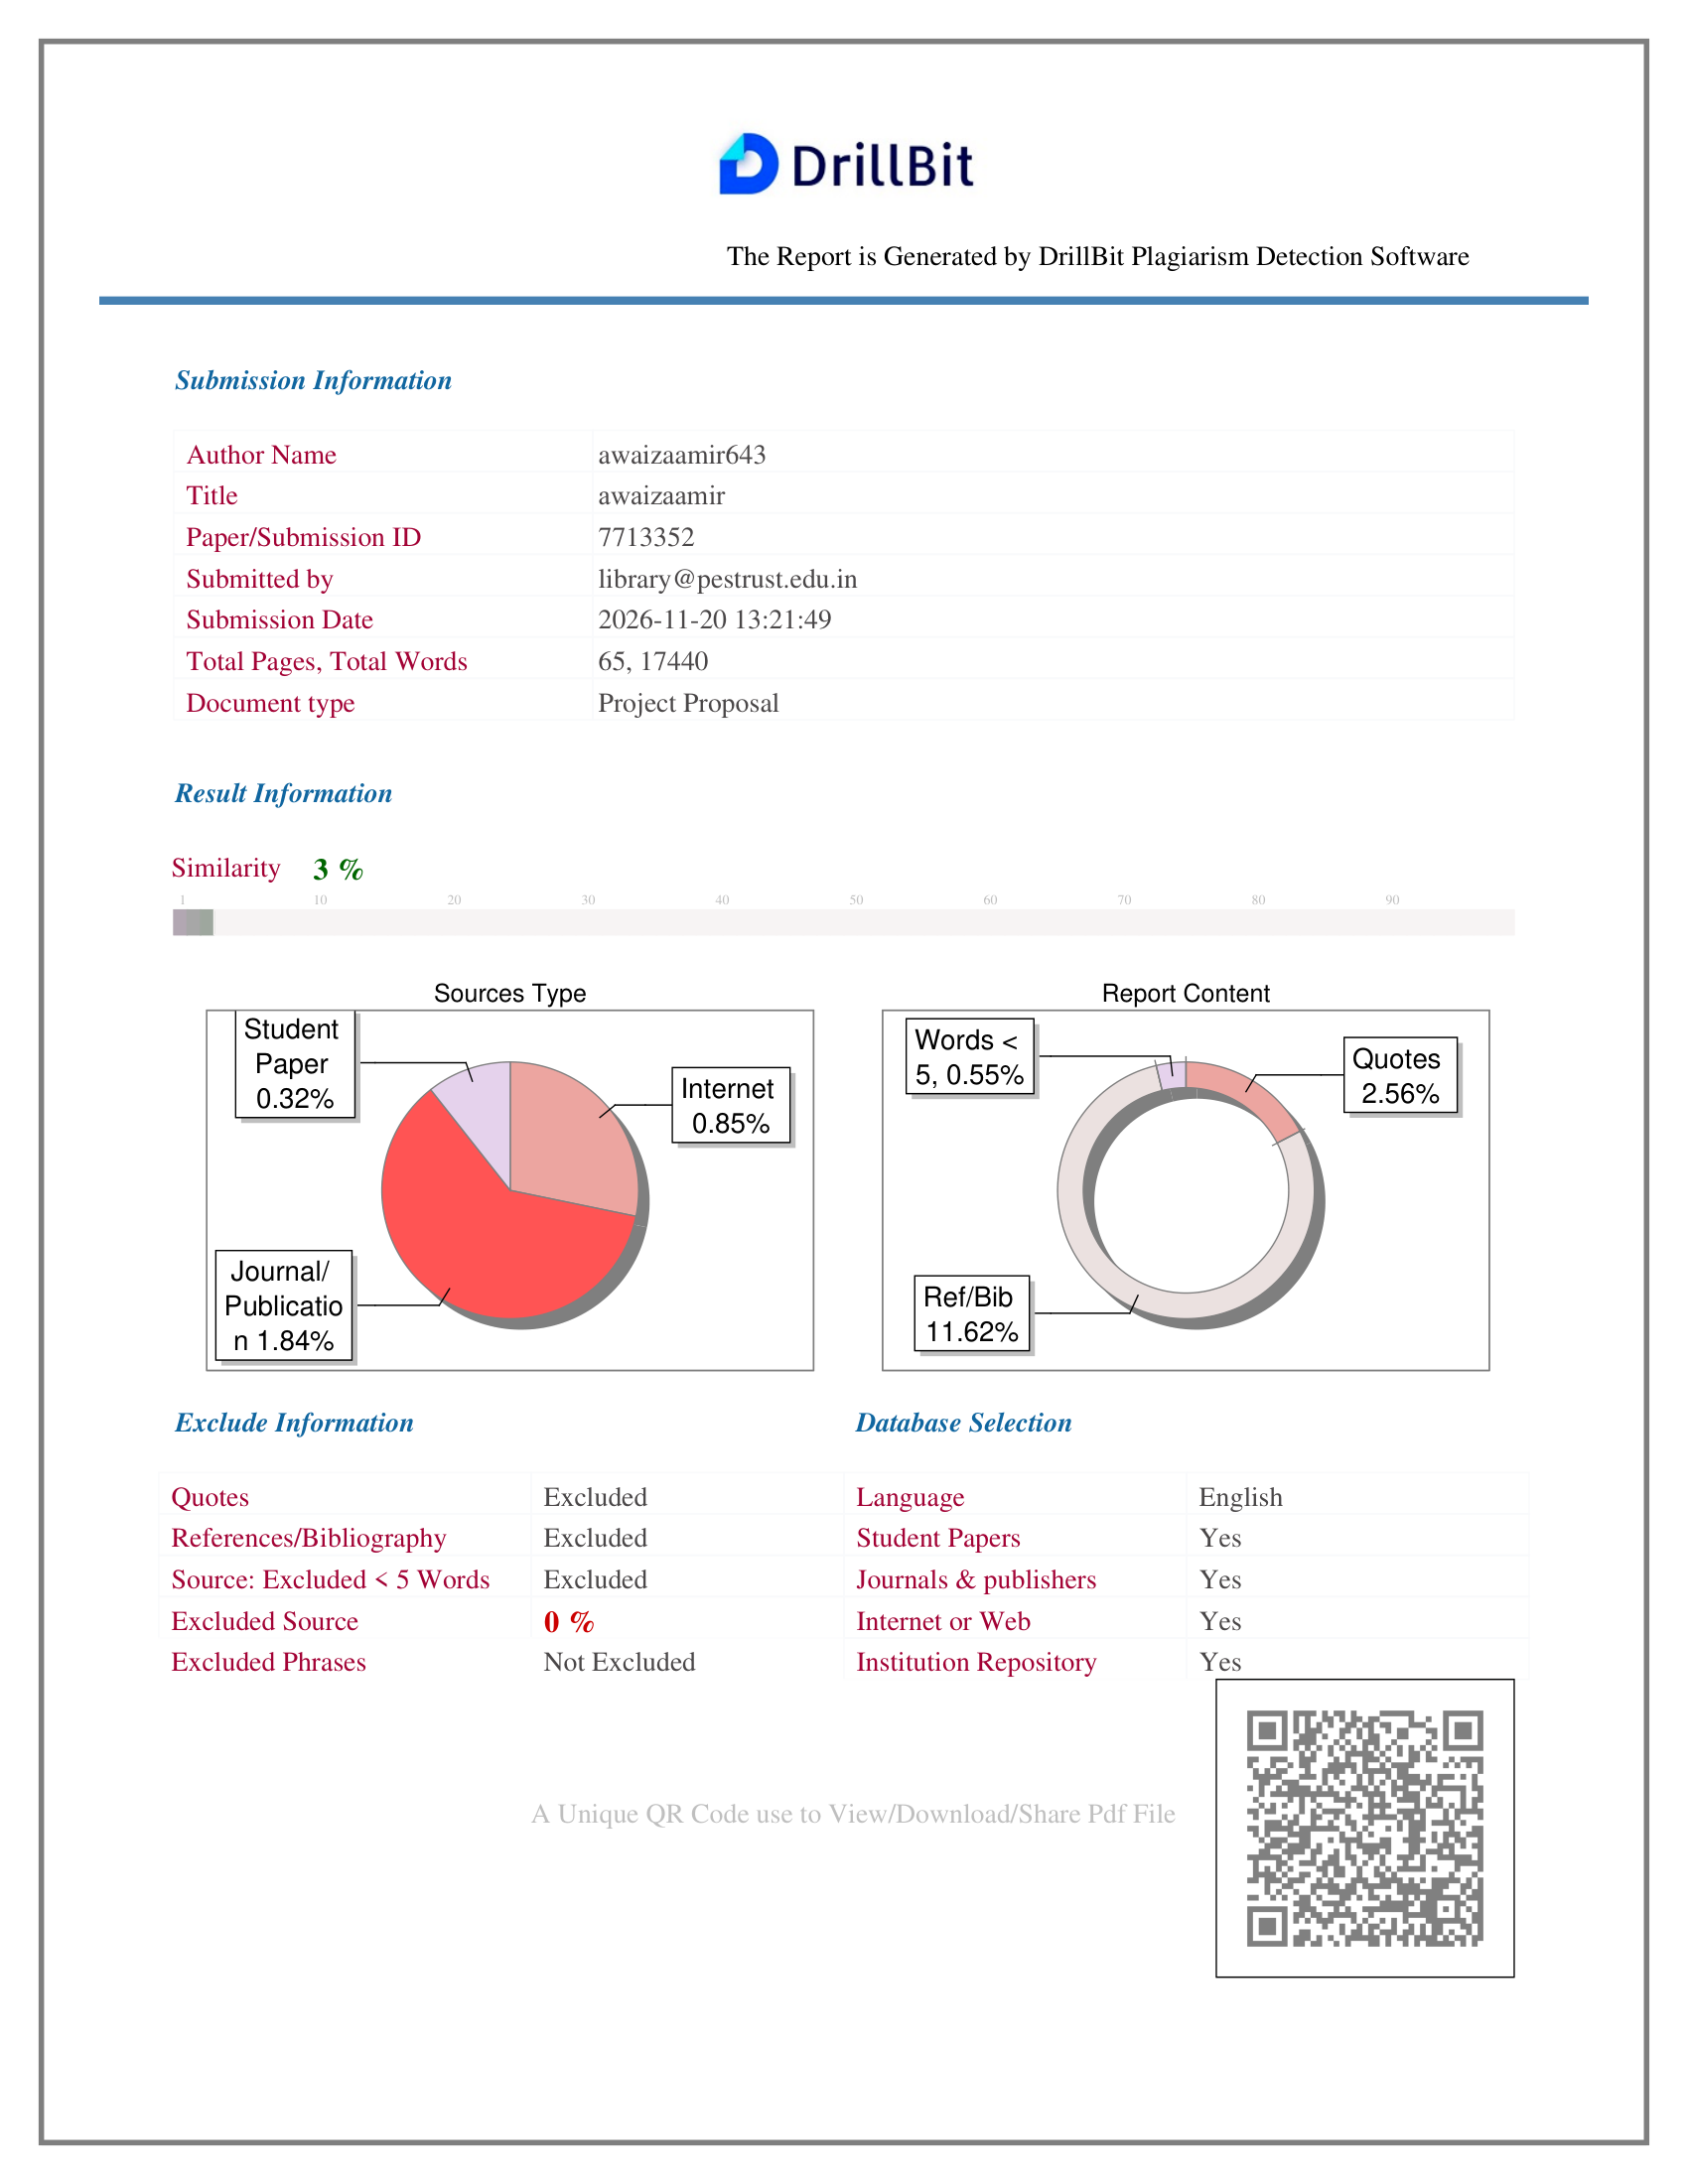
\includegraphics[width=0.92\textwidth]{drillbit_report.png}
    \caption{Official DrillBit Plagiarism Detection Report (Similarity Index: 3\%, Grade A)}
    \label{fig:drillbit_report}
\end{figure}


\end{document}
